\documentclass[12pt]{article}
\usepackage{import}
\usepackage{amsmath}
\usepackage{float}
\usepackage[utf8]{inputenc}
\usepackage{graphicx}
\usepackage{setspace}
\usepackage{enumitem}
\usepackage{multirow}
\usepackage{tabularx}
\usepackage[table,xcdraw]{xcolor}
\usepackage{array}
\usepackage{tocloft}
\usepackage{xcolor}
\usepackage{titlesec}
\usepackage{natbib}
\usepackage{caption}
\usepackage{appendix}
\usepackage[margin=0cm]{geometry}

\geometry{a4paper, portrait, margin=30mm, bmargin=30mm, tmargin=30mm}
\setcounter{secnumdepth}{5}
\setcounter{tocdepth}{5}
\setlength\parindent{0pt}

\makeatletter
\newcommand\subsubsubsection{\@startsection{paragraph}{4}{\z@}{-2.5ex\@plus -1ex \@minus -.25ex}{1.25ex \@plus .25ex}{\normalfont\normalsize\bfseries}}
\titleformat{\subsubsubsection}{\normalfont\bfseries}{\arabic{subsubsubsection}.}{0.5em}{}  
\newcommand\subsubsubsubsection{\@startsection{subparagraph}{5}{\z@}{-2.5ex\@plus -1ex \@minus -.25ex}{1.25ex \@plus .25ex}{\normalfont\normalsize\bfseries}}
\titleformat{\subsubsubsubsection}[hang]{\normalfont\bfseries}{\thesubsubsubsection\arabic{subsubsubsubsection}.}{0.5em}{}  
\makeatother
\renewcommand{\thesection}{\Roman{section}/}
\titleformat{\section}[hang]{\normalfont\Large\bfseries}{\thesection}{0.5em}{}
\setlength{\cftsecnumwidth}{2.5em} 
\setlength{\cftsecindent}{1.5em}
\renewcommand{\thesubsection}{\arabic{subsection}.}
\setlength{\cftsubsecindent}{3em}
\titleformat{\subsection}{\normalfont\bfseries}{\thesubsection}{0.5em}{}
\renewcommand{\thesubsubsection}{\thesubsection\arabic{subsubsection}}
\titleformat{\subsubsection}{\normalfont\bfseries}{\thesubsubsection}{0.5em}{}
\setlength{\cftsubsubsecindent}{5em}
\begin{document}
\setstretch{1.15}

%\vspace{10mm}  % vertical space
\thispagestyle{empty}
% \addvspace{5mm}  % vertical space until length

%$$$$$$$$$$$$$$$$$$$$$$$$$$$$$$$$$$$$$$$$$$$$$$$$$$$$$$$$$$$$$$$$$$$$$$$$$$$$$$$$$

\newgeometry{top=0.6in, bottom=0.6in, left=0.6in, right=0.6in}
% Make the title page
\begin{titlepage}
    \begingroup % Start a local scope
    \renewcommand{\baselinestretch}{1.75}\normalsize 
    \begin{center}
        % Draw a border around the entire page
        \setlength{\fboxrule}{1pt} 
        \setlength{\fboxsep}{2pt} 
        \fbox{
            \begin{minipage}[c][0.98\textheight][c]{0.98\textwidth} % Adjust content width
                \centering
                \vspace{-30mm} % Reduce vertical space at the top
                % University name and department
                \makebox[\textwidth][c]{\normalsize \textbf {UNIVERSITY OF SCIENCE AND TECHNOLOGY OF HANOI}} \\[5pt]
                \makebox[\textwidth][c]{\normalsize \textbf {DEPARTMENT OF INFORMATION AND COMMUNICATION TECHNOLOGY}} \\[20pt]
            
                % USTH logo
                
\includegraphics[width=0.5\textwidth]{image/usth.png} \\[15pt]
            
                % Report title
                \textbf{\LARGE GROUP PROJECT REPORT} \\[3pt]
                \textbf{\fontsize{19}{22}\selectfont USTH Connect}\\
                \textbf{\fontsize{19}{22}\selectfont Integrated app for university life assistant \\ and student networking} \\[30pt]
            
                % Group members section
                \textbf{\large Group Members} \\[10pt]
                \begin{tabular}{l@{\hskip 3cm}l} % Add spacing of 3cm between columns
                Nguyen Thi Van    & 22BI13459 \\
                Chu Hoang Viet     & 22BI13462 \\
                Nguyen Hoai Anh        & 22BI13021 \\
                Nguyen Dang Nguyen & 22BI13340 \\
                Do Minh Quang           & 22BI13379 \\
                \end{tabular} \\[20pt]
            
                % Supervisor section
                \textbf{\large Supervisor} \\[3pt]
                Assoc. Prof. Tran Giang Son \\[20pt]
            
                % Footer
                \textbf{January, 2025}
            \end{minipage}
        }
    \end{center}
    \endgroup % End local scope
\end{titlepage}

% Restore margins for the rest of the document
\restoregeometry

\thispagestyle{empty}

% end of title page
%$$$$$$$$$$$$$$$$$$$$$$$$$$$$$$$$$$$$$$$$$$$$$$$$$$$$$$$$$$$$$$$$$$$$$$$$$$$$$$$$$
\newpage
\renewcommand{\listfigurename}{LIST OF FIGURES}
\renewcommand{\cftloftitlefont}{\Large\bfseries} 
\renewcommand{\cftafterloftitle}{
    \par\noindent\vspace{-0.5em}
    \textcolor{blue}{\rule{\textwidth}{0.5pt}}
    \vspace{1em} 
}
\renewcommand{\cftfigpresnum}{Figure~}
\renewcommand{\cftfigaftersnum}{:}
\setlength{\cftfignumwidth}{5em}


\renewcommand{\contentsname}{\centering TABLE OF CONTENTS}
\begin{center}
    \tableofcontents
\end{center}
\newpage

\section*{Acknowledgement}
\addcontentsline{toc}{section}{Acknowledgement}
\noindent The opportunity to do this project at
the University of Science and Technology of Hanoi, Vietnam
was an arrow in the quiver of our career. We appreciate
this great chance to work professionally beside outstanding researchers.\\
\\

We would like to express our gratitude to our 
supervisor, Dr. TRAN Giang Son for his precious 
guidance and support throughout the project. Our
project would not have been possible without his
constructive instruction. \\
\\

We would also like to thank our team members for 
their continuous contributions, hard-working and brilliant ideas, 
which led us through the project successfully.\\
\\

Last but not least, we would like to thank our family 
and friends for their unwavering support and encouragement
throughout our project.



\newpage
\vspace{2em}
\section*{LIST OF ABBREVIATIONS}
\addcontentsline{toc}{section}{List of Abbreviations}
\vspace{-0.9em}
\textcolor{blue}{\rule{\textwidth}{0.5pt}} 
\vspace{1em}
\begin{tabbing}
    \hspace{4cm} \= \hspace{10cm} \kill
    \textbf{API} \> Application Programming Interface \\
    \textbf{RBAC} \> Role-Based Access Control \\
    \textbf{JWT} \> JSON Web Token \\
    \textbf{VoIP} \> Voice over Internet Protocol \\
    \textbf{VPN} \> Virtual Private Network \\
    \textbf{K-modes} \> K-modes Clustering Algorithm \\
    \textbf{SIP} \> Session Initiation Protocol \\
    \textbf{TLS} \> Transport Layer Protocol \\
    \textbf{UAC} \> User Agent Client \\
    \textbf{UAS} \> User Agent Server \\
    \textbf{URI} \> Uniform Resource Identifier \\
    \textbf{DBI} \> Davies-Bouldin Index \\
    \textbf{ORM} \> Object-Relational Mapping \\
    \textbf{JPA} \> Java Persistence API
\end{tabbing}

\newpage
\listoffigures
\addcontentsline{toc}{section}{List of Figures}
\renewcommand{\listtablename}{LIST OF TABLES}
\renewcommand{\cftlottitlefont}{\Large\bfseries} 
\renewcommand{\cftafterlottitle}{
    \par\noindent\vspace{-0.5em}
    \textcolor{blue}{\rule{\textwidth}{0.5pt}}
    \vspace{1em} 
}
\renewcommand{\cfttabpresnum}{Table~}
\renewcommand{\cfttabaftersnum}{:}
\setlength{\cfttabnumwidth}{5em}
\newpage

\listoftables
\addcontentsline{toc}{section}{List of Tables}
\newpage
\section*{Abstract}
\addcontentsline{toc}{section}{Abstract}
\noindent University life
especially for first-year students, involves several 
challenges, including managing academic timetables, 
finding study resources, locating buildings in the campus, 
and builing connections between students. In order to address these 
issues, USTH Connect, an integrated University 
Life Assistant and Student Networking App, 
was developed. This Android application utilizing the advanced technologies to improve access to academic calendars, 
study materials, and campus' buildings navigation, 
while also encouraging connections 
via the innovative StudyBuddy function. 
By utilizing the K-modes clustering model, the app will pair students with compatible study partners and enables communication through secure 
Linphone-powered VoIP audio calls and instant messaging.\\

\noindent In addition, we also use a centralized PostgreSQL database for data storage, data security. The software 
includes Google Calendar, MapBox, and Moodle, 
allowing for real-time updates, 
easier navigation, and fast resource access. 
USTH Connect aims to improve the university 
experience by simplifying academic tasks and 
encouraging contact between students. This report focuses 
on the application's design, development, and implementation, 
demonstrating how it solves issues while improving 
efficiency and connectivity in the academic 
environment.\\

\noindent \textbf{Keywords}: USTH Connect,
K-modes clustering, Linphone, Google Calendar, MapBox, Moodle



\newpage

\section{Introduction}

\subsection{Context and Motivation}
University students face many challenges, especially in their first year. Managing academic schedules, finding campus locations, accessing study materials, and forming social connections can be overwhelming.
While some universities provide tools to help, these systems are often fragmented and difficult to use. \\

Around the world, many existing apps have already addressed specific student needs. 
For example, Google Calendar helps with scheduling, Moodle provides lecture resources, Google Maps assists with navigation, and Google Classroom helps managing assignments and course updates.
However, these tools work separately and don’t provide a single platform that connects academics, social life, and campus navigation.
While Google Calendar does not help students connect with peers, Google Maps lacks academic support, and Moodle and Google Classroom do not offer campus navigation or social networking features.
This seperation makes it harder for students to handle everything in one place. \\

To overcome these challenges, we developed USTH Connect, an integrated University Life Assistant and Student Networking Application. 
USTH Connect is built with the goal of supporting students' university life by combining modern yet simple technologies into an Android application, providing students with effortless access to the schedules, study materials and study location addresses.
Not only does it support their studies, it also encourages more connections between students, supporting them in their social life. That helps them to create more quality and meaningful relationships in the future.
With StudyBuddy, students can find compatible study partners, chat, and even make audio calls through secure VoIP functionality powered by Linphone.
To support the StudyBuddy features, we apply the K-modes model to help students find compatible people in the university.
USTH Connect uses a secure PostgreSQL database to manage data centrally, ensuring both protection and efficiency.\\

Below is an illustration showing how USTH Connect connects to the other products mentioned above: 
\begin{figure}[H]
    \centering
    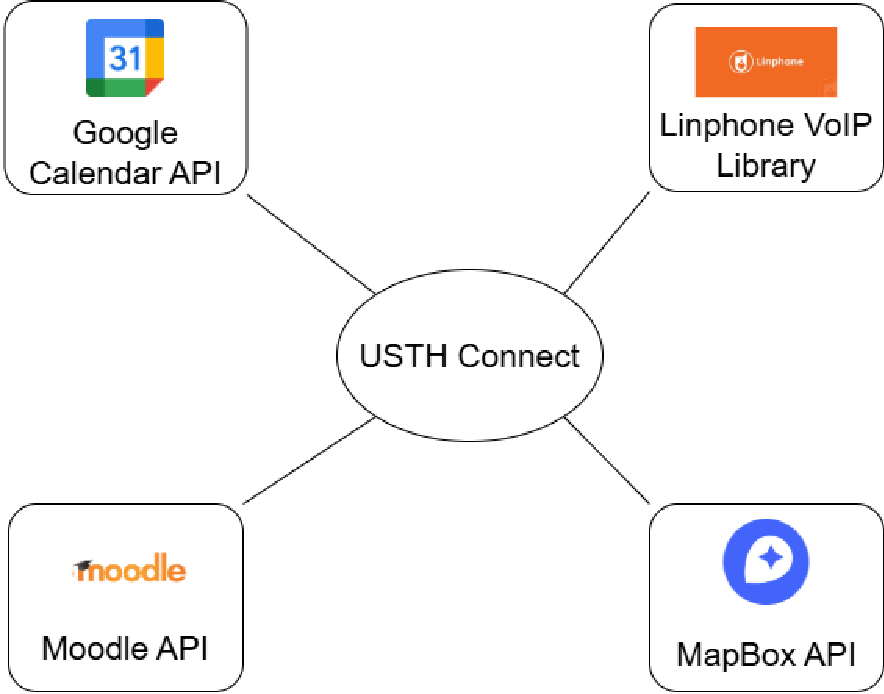
\includegraphics[width=0.7\textwidth]{image/Integration-USTH-Connect-External-Services.pdf} 
    \caption{Integration of USTH Connect with External Services}
    \label{fig:integration-external-services}
\end{figure}

This report explains the design and development of USTH Connect, highlights its features, and discusses the challenges we faced. 
It also shows how USTH Connect enhances the university experience for students.

\subsection{Project Objectives}
The primary objective of this project is to design, develop and implement an integrated system that enhances university life and fosters student networking through advanced technological solutions.
The goal is to create a platform that seamlessly intergrates personal academic data, event annoucements, and campus resources.
By using advanced frameworks and APIs, together with recommendation system, we aim to simplify the administrative tasks, improve campus accessibility, 
and encourage more interaction among students.
The platform will be accessible to students, making it easy for them to experience campus life, stay informed, and connect with friends.

\subsection{Desired Outcomes}  
The USTH Connect is expected to enhance the university experience by streamlining academic and social interactions for students and administrators.
To achieve that outcomes, we seamlessly integrate essential tools like schedules, course materials, and campus navigation.
The StudyBuddy feature, supported by machine learning, is aimed to effectively connect students with compatible learning partners, encourage cooperation between students, and enhance the student social life.
Linphone-powered chat and audio calls will facilitate seamless communication and strengthen social bonding among students.
Real-time notifications for calendar updates and events together with calling and messaging will keep users informed, organized and connected.
The integration of Google Calendar, MapBox, and Moodle promise a student-friendly experience across Android devices.
In summary, USTH Connect is supposed to significantly improve the university experience for students and administrators by encouraging a more efficient and connected academic environment.

\subsection{Structure of Report}
The report will be structured as follows:
\begin{itemize}
    \item \textbf{Part I: Introduction }
    \newline
    Provide a general introduction to the report, including an overview of the project, its objectives, and the scope of the work.
    \item \textbf{Part II: Requirement Analysis }
    \newline
    Lists all the tools, techniques, and system requirements used in the project. It includes
    both functional and non-functional requirements, as well as desired functionalities.
    \item \textbf{Part III: Methodologies }
    \newline
    System architecture, database design, and implementation details of various features, illustrated with sequence diagrams.
    \item \textbf{Part IV: Machine Learning Model Analysis and Training }
    \newline
    Analysis and training of AI models for recommend system for study buddy matchmaking, including datasets and model development, with (Model Name) integration.
    \item \textbf{Part V: System Design and Implementation }
    \newline
    Overview of the system's design and implementation process, detailing the hardware and software setups, core application modules, and the initial testing phases to ensure seamless integration and functionality.
    \item \textbf{Part VI: Results and Discussions }
    \newline 
    Summarizes the implementations and achievements of the system. It reflects on how the
    objectives were met and provides a summary of the project's outcomes.
    \item \textbf{Part VII: Conclusion and Future Work }
    \newline
    Reviews the project's successes in improving student life and fostering connections within the university.
    It also acknowledges the challenges encountered during development and identifies areas where the system could be further improved.
\end{itemize}

\pagebreak


\section{Requirement Analysis}
Ensuring and following the initial targets set for the project, we must be carefully analyzed the system
architecture and and implemented clear methodologies and procedures. Below is a detailed description of our approach.

\subsection{System requirements}
This section outlines the essential requirements for the development and successful operation of USTH Connect, classified into functional, non-functional, and desired functionalities.

\subsubsection{Functional Requirements}
The functional requirements specify the primary operations and features of USTH Connect to meet student and system objectives:  
\begin{itemize}  
    \item \textbf{Authenticate and Authorize:} Implement secure student authentication using JWT-based tokens and role-based access control (RBAC) for managing access permissions.  
    \item \textbf{Integrate with Google Calendar:} Enable users to sync, view, and manage academic schedules in real-time within the application.  
    \item \textbf{Match with StudyBuddy:} Allow students to find study partners based on shared academic interests, goals, and compatibility through machine learning algorithms.  
    \item \textbf{Access Moodle Resources:} Provide seamless access to course materials, including slides, assignments, and reference documents, fetched directly from Moodle.  
    \item \textbf{Send Real-time Notifications:} Notify users promptly about calendar updates, study partner incoming communication, and scheduled events.  
    \item \textbf{Display Map and Navigation:} Integrate MapBox to display campus maps, building locations, and navigation features for easy campus exploration.  
    \item \textbf{Enable Communication Features:} Facilitate text-based chatting and VoIP audio calls using Linphone for seamless interaction between users.  
    \item \textbf{Provide Administrative Tools:} Offer reporting tools for administrators to monitor student engagement, system usage.  
\end{itemize} 

\pagebreak

\subsubsection{Non-functional Requirements}
The non-functional requirements outline the system's essential performance, reliability, and usability standards. While official testing has not yet been carried out, the following testing are planned to validate each requirement:
\begin{itemize}
    \item \textbf{Scalability:} The system should support a moderate increase in student numbers and data while maintaining acceptable performance levels. 
    To perform test on the increase of users, we plan to use Apache JMeter or Locust to simulate growth usage, scaling up to around 130\% of the current user load. 
    These tests will focus on some important functionalities like schedule retrieval and display for each major, resources view, and StudyBuddy matching, in order to verify that performance of the application is stable and working well with a 30\% increase in user numbers.

    \item \textbf{Security:} User data must be protected with basic encryption protocols, secure database practices (PostgreSQL). 
    To test the security of the system, we plan to use OWASP ZAP to perform penetration testing and security audits. 
    By taking advantages of the tools, we will simulate attacks, such as SQL injection and data interception, will be held to analyze and identify upcoming potential vulnerabilities to the system.
    These tests will focus on the robust security of sensitive information and how the system will act when facing against unauthorized access attempts.

    \item \textbf{Availability:} The system should aim for an uptime of at least 90\%, ensuring minimal disruption to student access. 
    To validate this, we plan to perform tests which involve of simulating a situation like a high user usage and resource demand during peak usage times.
    By using automated tools and performing a test around 30 days, we will check for the stability of the system behavior and uptime in these specific scenarios.
    These tests will ensure to meet the target uptime we mention above and to maintain the reliable access for users.

    \item \textbf{Performance:} Key functionalities, such as schedule retrieval and StudyBuddy matching, should respond within 5 seconds under normal conditions. 
    To verify this, we plan to take advantages of libraries like Microbenchmark and Macrobenchmark to simulate the performance benchmarking. 
    By dividing into different levels of concurrent user (e.g., 10, 50, and 100 users), we will apply the test for each levels to observe response time for these key features.
    The goal is to ensure that the response time will be around 5 seconds for at least 90\% of all functionalities during typical and crowded conditions.

    \item \textbf{Usability:} The interface should be straightforward and functional, providing a smooth experience on most Android devices. 
    To test the usability, we plan to perform with a sample group of students who will be asked perform common tasks, such as retrieving schedules, acessing resources, and finding StudyBuddies. 
    Then through surveys and interviews, we can collect the feedback which will be used to identify areas for improvement. 
    The goal is for at least 80\% of participants to feel satisfied with the interface and find it functional and easy for them to use.

    \item \textbf{Maintainability:} Updates and feature additions should be feasible without causing significant downtime or compatibility issues. 
    To test the maintainability of the system, we plan to simulate updates in a controlled development environment. This involve introducing new features or patches while performing all the above testing to ensure that all functionalities are working as expected.
    During the maintenance, we will also observe the update process for any potential errors, such as compatibility errorso or longer downtime. 
    These tests will verify that the updates can be applied correctly with minimal interruption.
\end{itemize}

\subsubsection{Desired Functionalities}
These functionalities are not critical but aim to enhance the overall student experience and system capabilities:  
\begin{itemize}  
    \item \textbf{Personalized Dashboard:} Provide a customizable home screen with quick access to frequently used features, such as schedules, notifications, and StudyBuddy matches.  
    \item \textbf{Event Reminders:} Enable automated reminders for upcoming deadlines, meetings, and academic events.  
    \item \textbf{Offline Mode:} Allow limited functionality, such as viewing previously synced schedule, campus location and resources link, when the student is offline.  
    \item \textbf{User Feedback System:} Incorporate feedback and rating mechanisms for StudyBuddy matches and overall app experience.  
    \item \textbf{Cross-platform Compatibility:} Develop future support for IOS devices and web browsers to expand student accessibility.  
\end{itemize}  

\pagebreak

\subsection{Use Case}
Based on the use case diagram, this section will offer a general explanation of the system's
features.

\subsubsection{Use Cases Diagram}
    The below diagram is to demonstrate the interaction between users and system:
    % Figure
    \begin{figure}[H]
        \centering
       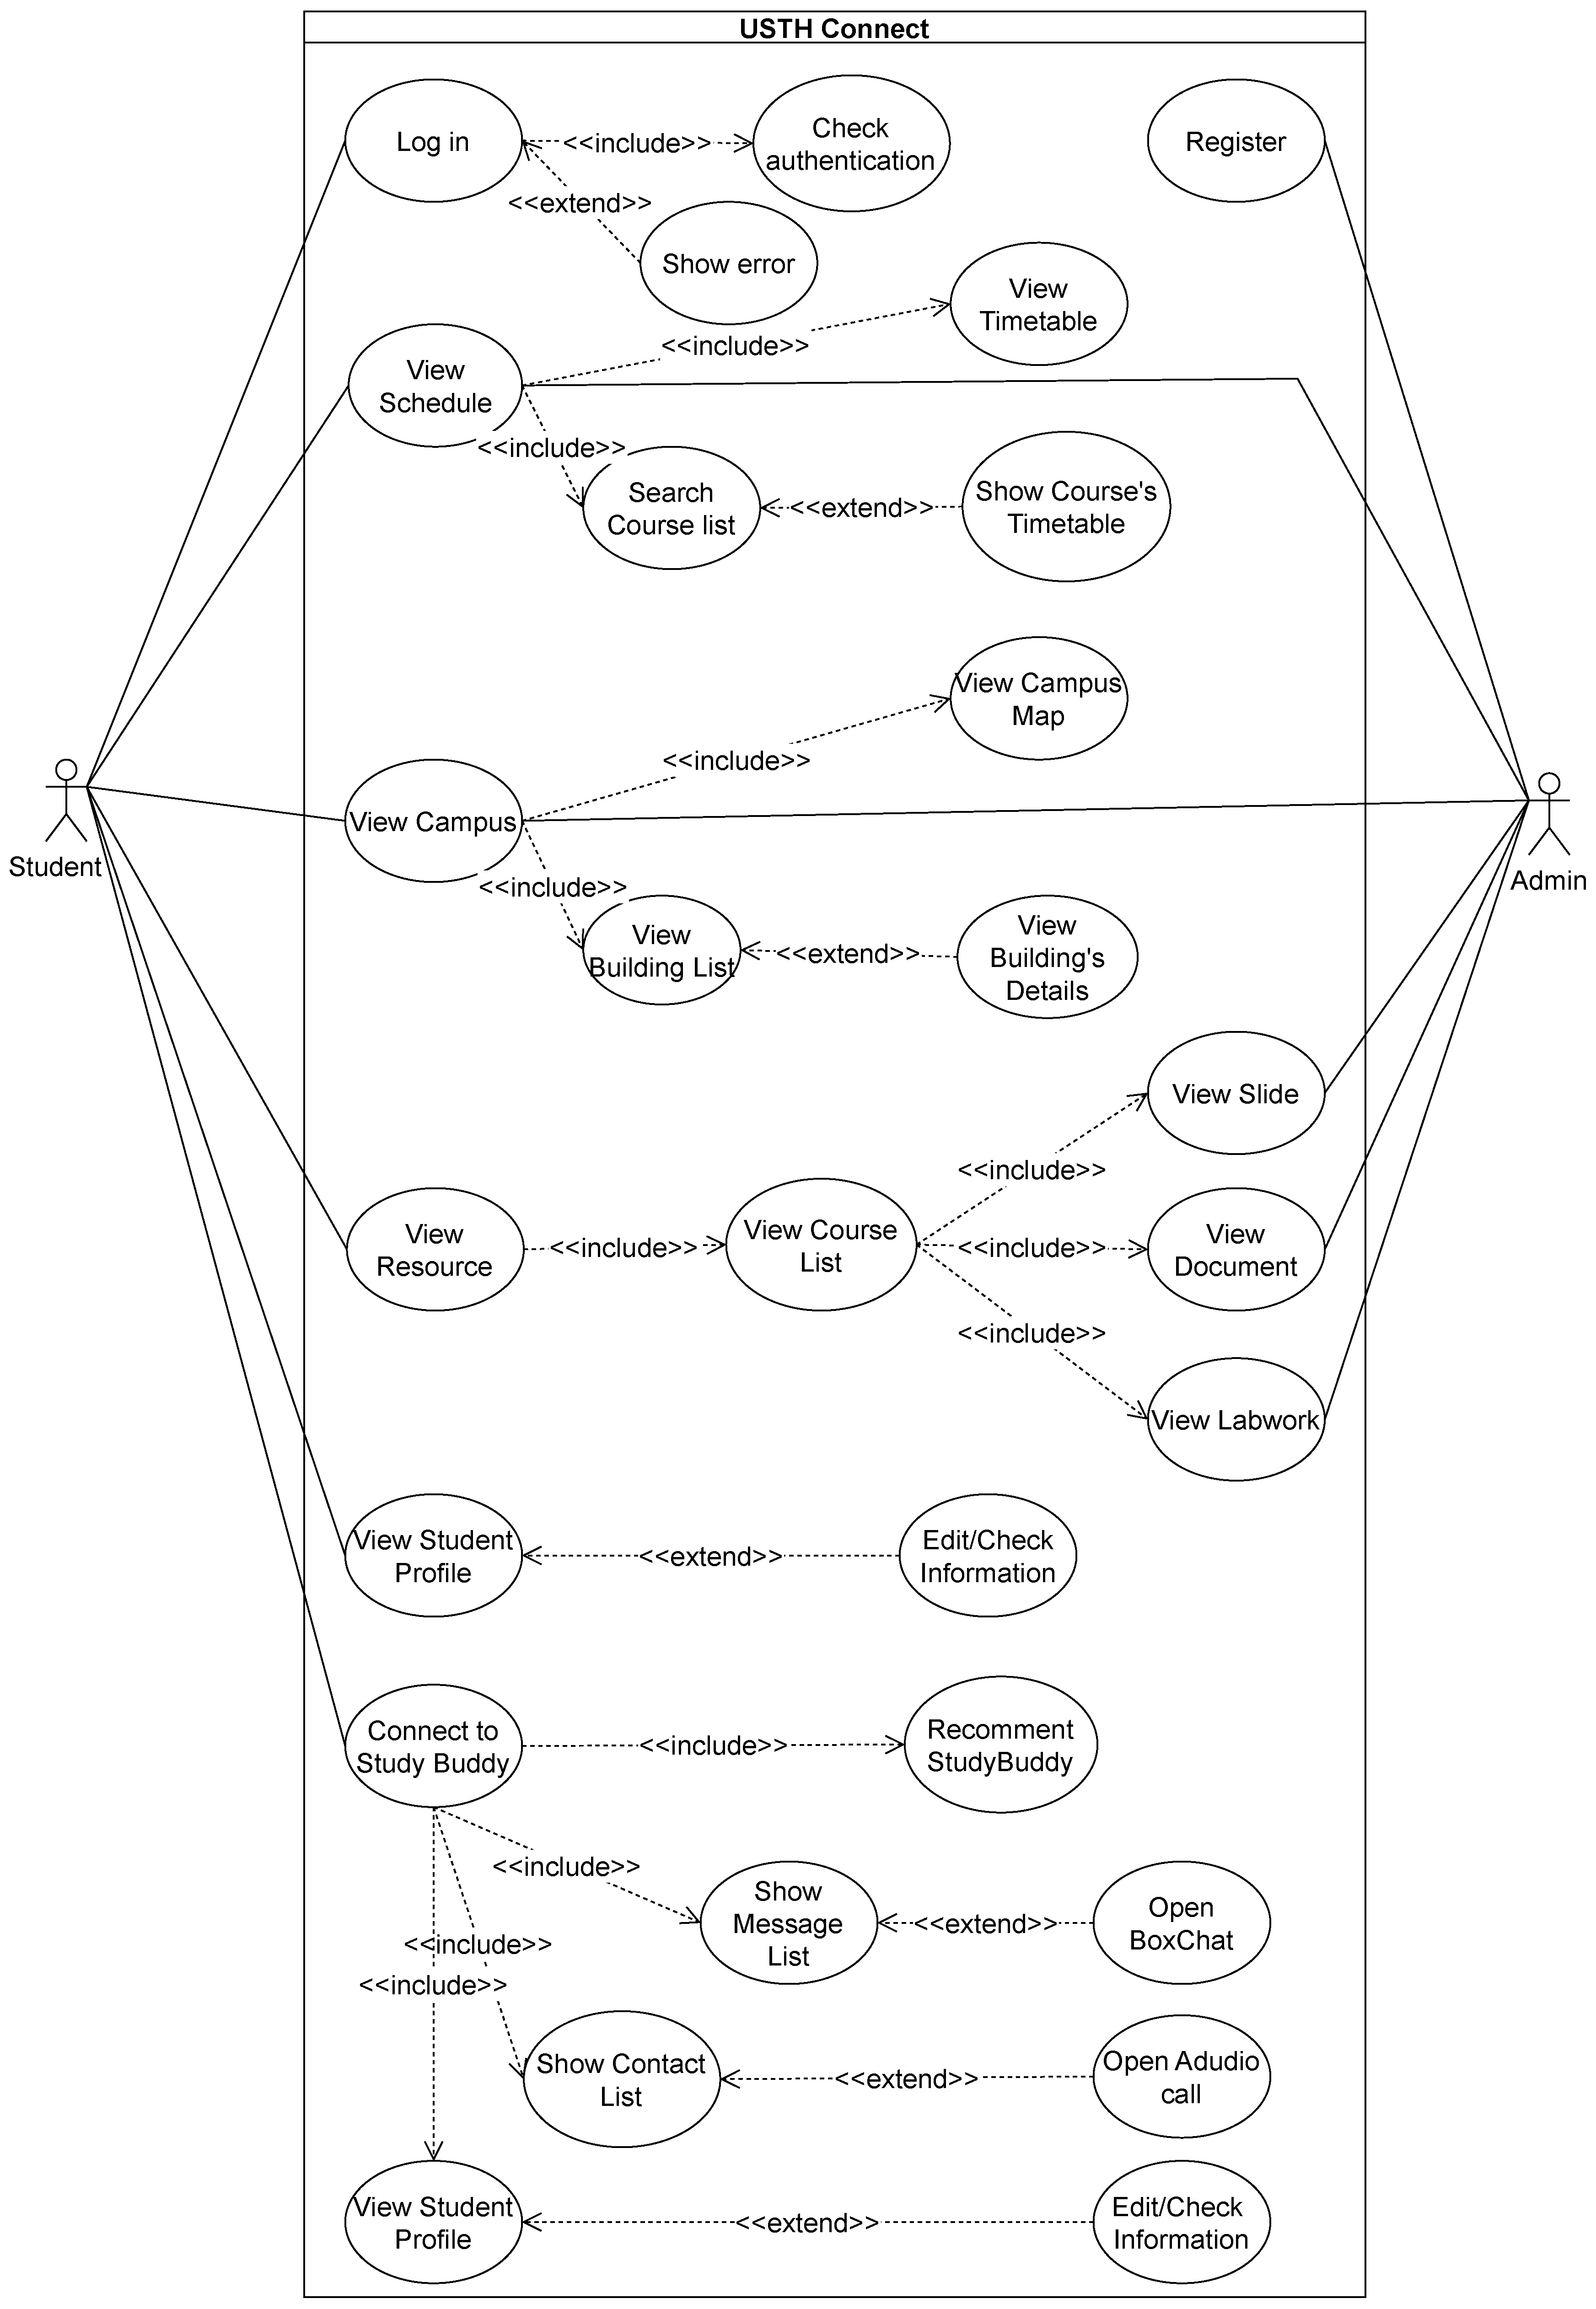
\includegraphics[width=0.8\textwidth]{image/USTHConnect_usecase_diagram.pdf} 
        \caption{Use case diagram}
        \label{fig:usthconnect_use_case}
    \end{figure}

    \pagebreak

\subsubsection{Use Case Characteristics}
    The system in Figure above has two roles: \textbf{Admin} and \textbf{Student}:
    \begin{itemize}
        \item \textbf{Admin:} Admins have access to all students' functionalities. 
        Additionally, they can manage schedules, campus, resources and create and manage student accounts.
        \item \textbf{Student:}  Students can login, reset their password. They have permission to check their schedule, university campus and resources. Additionally, they can connect to other students, who share the same interests, subjects, hobbies,  by using StudyBuddy.
    \end{itemize}

\subsection{Use Case and Scenario Description}
    This section provides a detailed description of the various use cases and scenarios within the USTH Connect application. 
    Each use case outlines the interactions between students and the system, describing how the system responds to specific student actions. \\
    
\textbf{Use case: Authenticate} \\

    \begin{figure}[H]
        \centering
        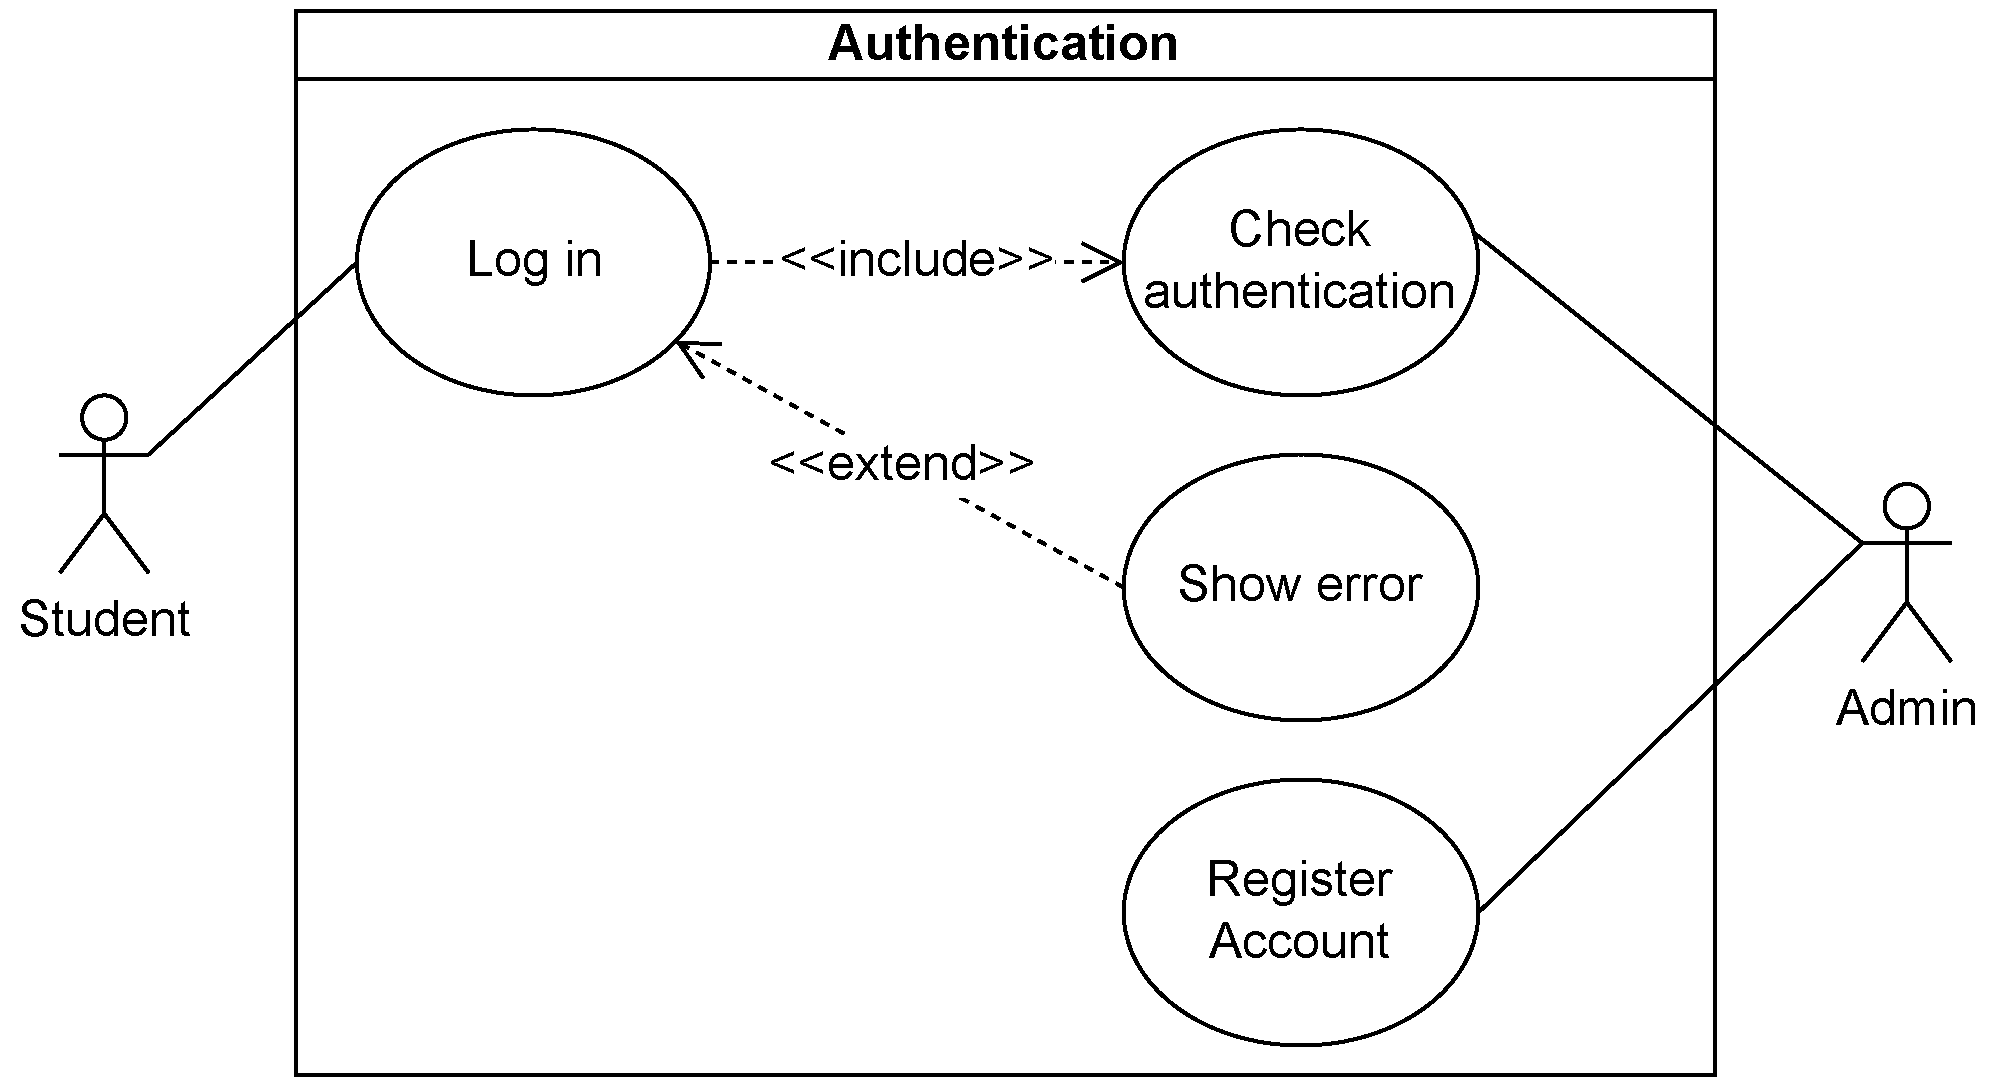
\includegraphics[width=0.7\textwidth]{image/AuthenticationUseCase.pdf} 
        \caption{Authentication use case diagram}
        \label{fig:authenticate_use_case}
    \end{figure}
    \textbf{Description:} Students can login and reset their passwords in case they forget them. Admin has to create accounts for students. \\

    \noindent \textbf{Pre-conditions:} Before this use case begins, students must ensure that all system packages are fully installed to avoid errors. \\

    \noindent \textbf{Post-conditions:}
    \begin{itemize}
        \item \textbf{Success:} Students can access the main screen.
        \item \textbf{Failure:} Not displaying the main screen, error message is shown in the system.
    \end{itemize}

    
    \begin{table}[H] 
        \centering
        \renewcommand{\arraystretch}{1.5}
        \begin{tabular}{|m{3.5cm}|p{10cm}|} 
            \hline
            \multicolumn{1}{|c|}{\textbf{Actor Action}} & \multicolumn{1}{c|}{\textbf{System Action}} \\ \hline
            & 1. Students enter studentID and password given by Admin \\ \cline{2-2} 
            \multirow{4}{=}{\centering \shortstack[c]{Login to the system \\ (User)}} 
            & 2. System verifies studentID and password against the stored database \\ \cline{2-2}
            & 3. If both studentID and password are correct, the system grants access to the student and displays the main screen \\ \cline{2-2}
            & 4. If it is incorrect, the system displays an error message and asks students to re-enter \\ \hline
            & 1. Student enters studentID and old password \\ \cline{2-2}
            \multirow{5}{=}{\centering \shortstack[c]{Change Password \\ (User)}} 
            & 2. System verifies studentID and password against the stored database \\ \cline{2-2}
            & 3. If the information entered is correct, students can change their password \\ \cline{2-2}
            & 4. System updates the new password in the database \\ \cline{2-2}
            & 5. Students enter the new password to login \\ \hline
        \end{tabular}
        \caption{Actor Actions and System Actions for Authenticate}
        \label{tab:authenticate_table}
    \end{table}

\textbf{Use case: Student Schedule} \\

    \begin{figure}[H]
        \centering
        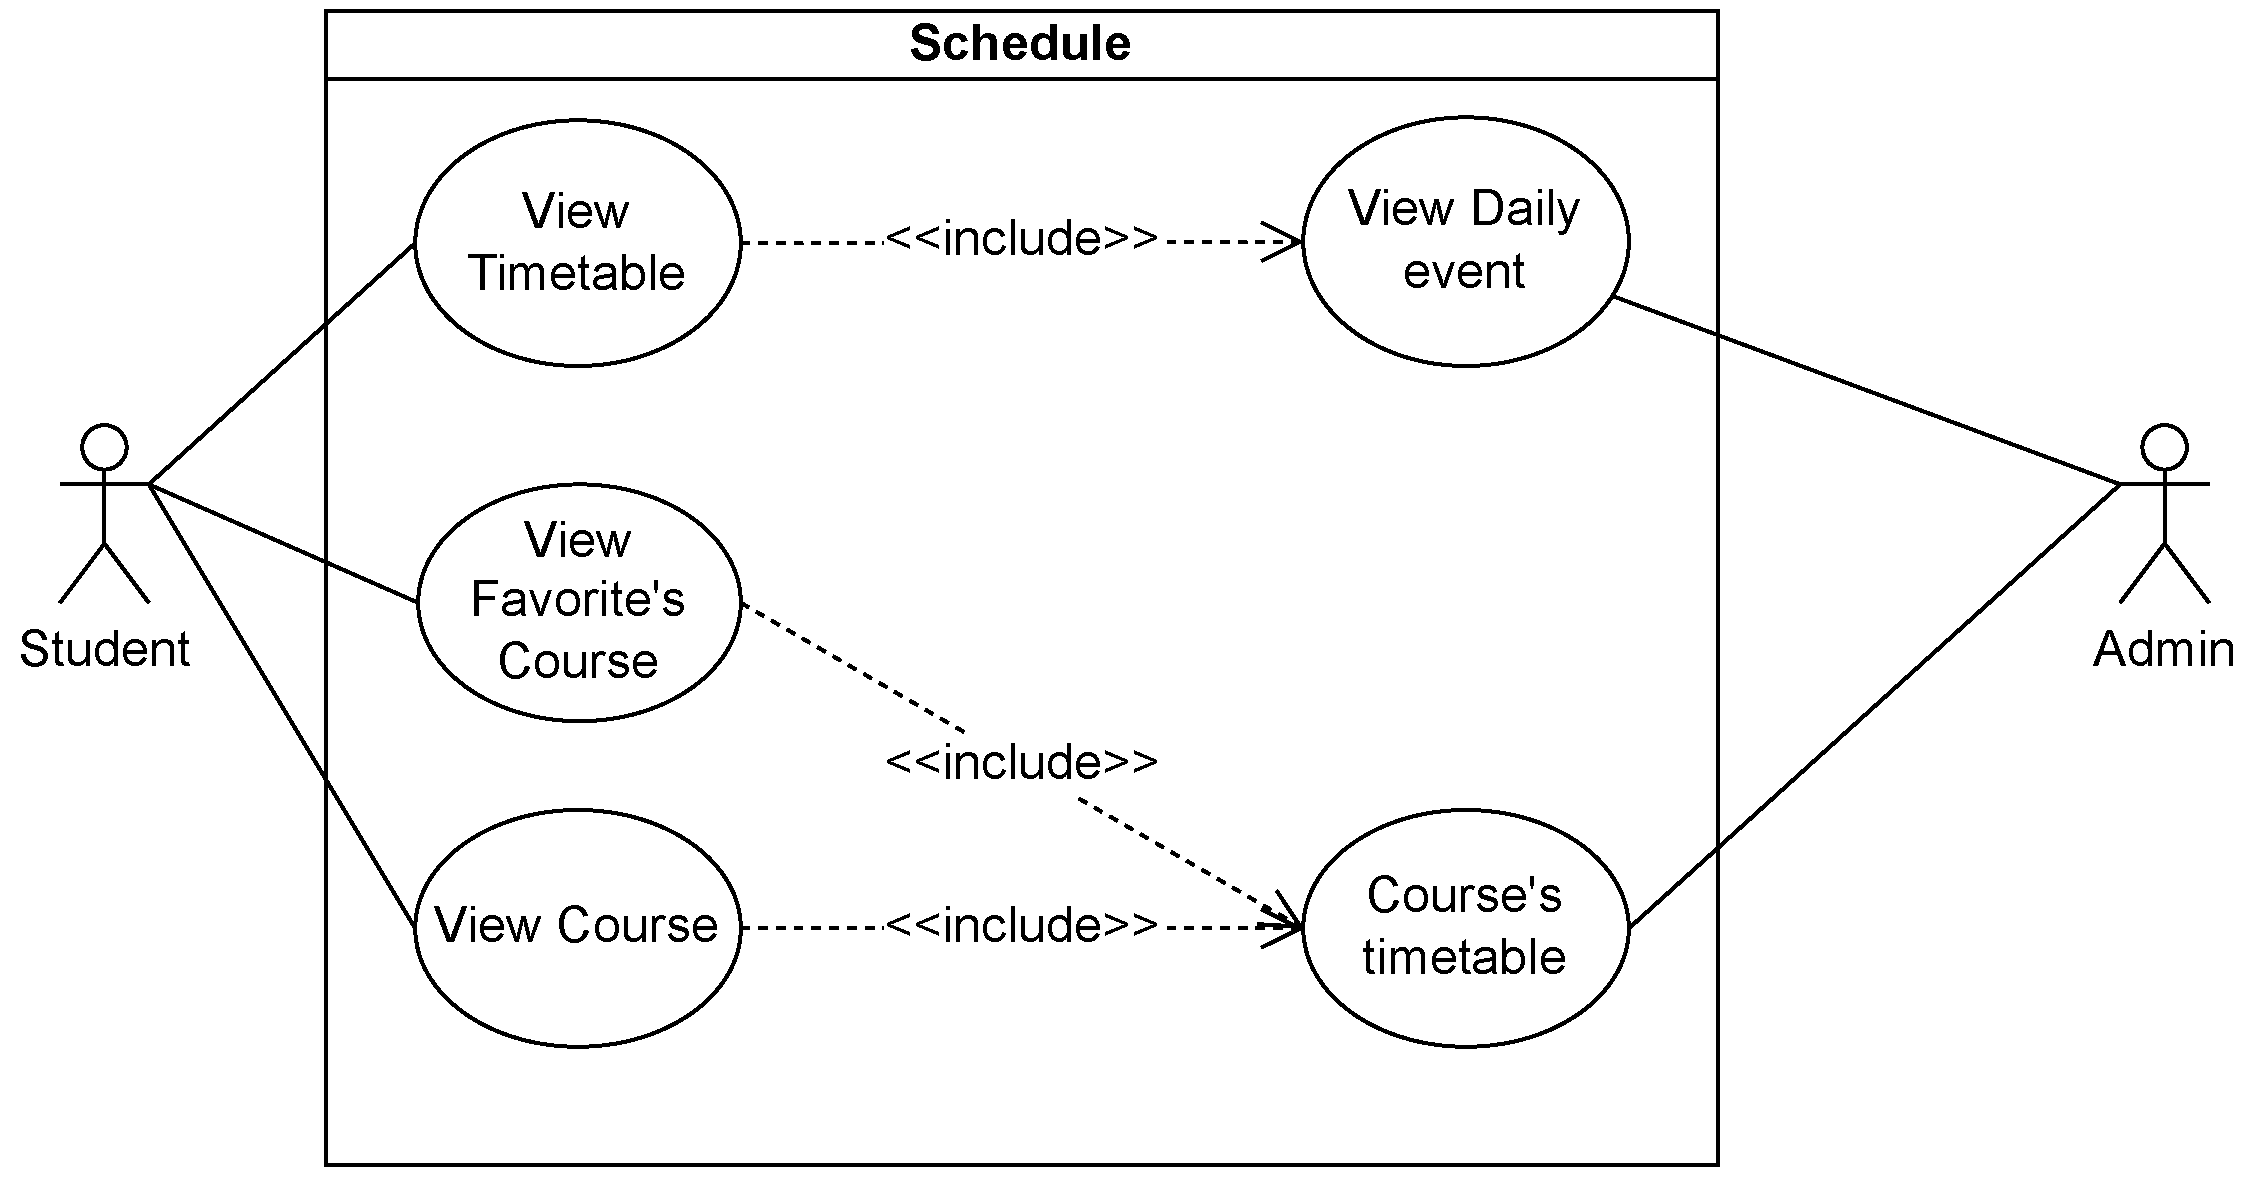
\includegraphics[width=0.7\textwidth]{image/StudentScheduleUseCase.pdf} 
        \caption{Schedule use case diagram}
        \label{fig:schedule_use_case}
    \end{figure}
    \textbf{Description:} This use case enables students to view their academic timetable. The system sync schedule every 10 minutes to make sure no daily event is missing. \\

    \pagebreak

    \noindent \textbf{Pre-conditions:} 
        \begin{itemize}
            \item Before this use case begins, students must be logged into the system.
            \item The system is up-to-date with course details: time, locations, lecturer.
        \end{itemize}

    \noindent \textbf{Post-conditions:}
    \begin{itemize}
        \item \textbf{Success:} 
        \begin{itemize}
            \item Students can see their daily events.
            \item System sends notification if there is a new class or a cancelled class.
        \end{itemize}
        \item \textbf{Failure:} Not display the event daily and show error messages.
    \end{itemize}

    \begin{table}[H]
        \centering
        \renewcommand{\arraystretch}{1.5}
        \begin{tabular}{|m{3.5cm}|p{10cm}|} 
            \hline
            \multicolumn{1}{|c|}{\textbf{Actor Action}} & \multicolumn{1}{c|}{\textbf{System Action}} \\ \hline
            \multirow{3}{=}{\centering \shortstack[c]{User click button \\ "Timetable"}} 
            & 1. The system shows a calendar \\ \cline{2-2} 
            & 2. Students can change the day, week, month format in the calendar \\ \cline{2-2}
            & 3. After choosing a day, students can see daily events \\ \hline
            \multirow{3}{=}{\centering \shortstack[c]{User click button \\ "Favorite Course"}} 
            & 1. The system shows a list of favorite courses which are added by Students \\ \cline{2-2}
            & 2. Students can see the timetable of their favorite course after clicking it \\ \cline{2-2}
            & 3. Un-click the favorite icon, the system will delete that course out of the list of favorite courses \\ \hline
            \multirow{3}{=}{\centering \shortstack[c]{User click button \\ "Course"}} 
            & 1. The system shows all the courses which match with the student’s major and year \\ \cline{2-2}
            & 2. Students can see the course class timetable after clicking the course \\ \cline{2-2}
            & 3. Click the favorite icon, the system will add that course to the list of favorite courses and show them in Favorite Course \\ \hline
        \end{tabular}
        \caption{Actor Actions and System Actions for Schedule}
        \label{tab:schedule_table}
    \end{table}

\pagebreak

\textbf{Use case: University Campus} \\

    \begin{figure}[H]
        \centering
        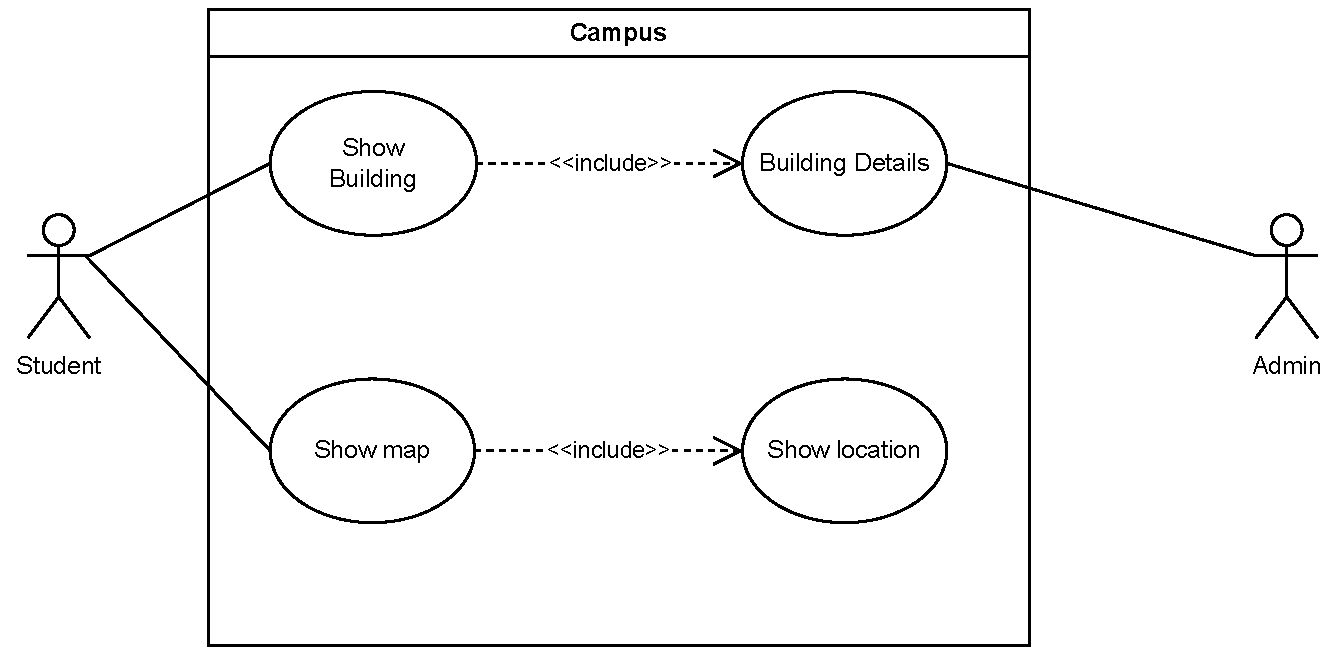
\includegraphics[width=0.7\textwidth]{image/CampusUseCase.pdf} 
        \caption{Campus use case diagram}
        \label{fig:campus_use_case}
    \end{figure}
    \textbf{Description:} The system displays a list of campus buildings and their details. The system can locate each building in a list on a map. \\

    \noindent \textbf{Pre-conditions:} 
        \begin{itemize}
            \item Before this use case begins, students must be logged into the system.
            \item Building data must be fetched from the database.
        \end{itemize}

    \noindent \textbf{Post-conditions:}
    \begin{itemize}
        \item \textbf{Success:} 
        \begin{itemize}
            \item Students can search for buildings on campus and each details.
            \item System shows a map where the student and building are located.
        \end{itemize}
        \item \textbf{Failure:} The system displays an error message or map fails to load.
    \end{itemize}

    \begin{table}[H]
        \centering
        \renewcommand{\arraystretch}{2.5}
        \begin{tabular}{|m{3.5cm}|p{10cm}|} 
            \hline
            \multicolumn{1}{|c|}{\textbf{Actor Action}} & \multicolumn{1}{c|}{\textbf{System Action}} \\ \hline
            \multirow{2}{=}{\centering \shortstack[c]{User click button \\ "Building"}} 
            & 1. The system shows a list of buildings which students study in \\ \cline{2-2} 
            & 2. After clicking a building, the system returns its details \\ \hline
            \multirow{1}{=}{\centering \shortstack[c]{User click button \\ "Map"}} 
            & 1. System loads a map to locate your location and each building \\ \hline
        \end{tabular}
        \caption{Actor Actions and System Actions for Campus}
        \label{tab:campus_table}
    \end{table}

\textbf{Use case: University Resource} \\

    \textbf{Description:} Students can access lectures, slides, exercises and homework from all bachelor’s programs, which the system displays. \\

    \noindent \textbf{Pre-conditions:} 
        \begin{itemize}
            \item Before this use case begins, students must be logged into the system.
            \item Lectures, slides, exes and homeworks must be fetched successfully.
        \end{itemize}
    \noindent \textbf{Post-conditions:}
    \begin{itemize}
        \item \textbf{Success:} Students can access and download all resources from all bachelor’s programs.
        \item \textbf{Failure:} The system displays an error message or resource fail to open or fail to load data.
    \end{itemize}

    \begin{table}[H]
        \centering
        \renewcommand{\arraystretch}{2.5}
        \begin{tabular}{|m{3.5cm}|p{10cm}|} 
            \hline
            \multicolumn{1}{|c|}{\textbf{Actor Action}} & \multicolumn{1}{c|}{\textbf{System Action}} \\ \hline
            \multirow{2}{=}{\centering \shortstack[c]{User click button \\ "Show Resource"}} 
            & 1. The system displays a list of bachelor’s programs \\ \cline{2-2} 
            & 2. After choosing bachelor’s programs, the screen shows majors, then, the system shows the subject of the major and lectures, slides, … of a subject of major \\ \hline
        \end{tabular}
        \caption{Actor Actions and System Actions for Resource}
        \label{tab:resource_table}
    \end{table}

\pagebreak

\textbf{Use case: Student StudyBuddy} \\

    \begin{figure}[H]
        \centering
        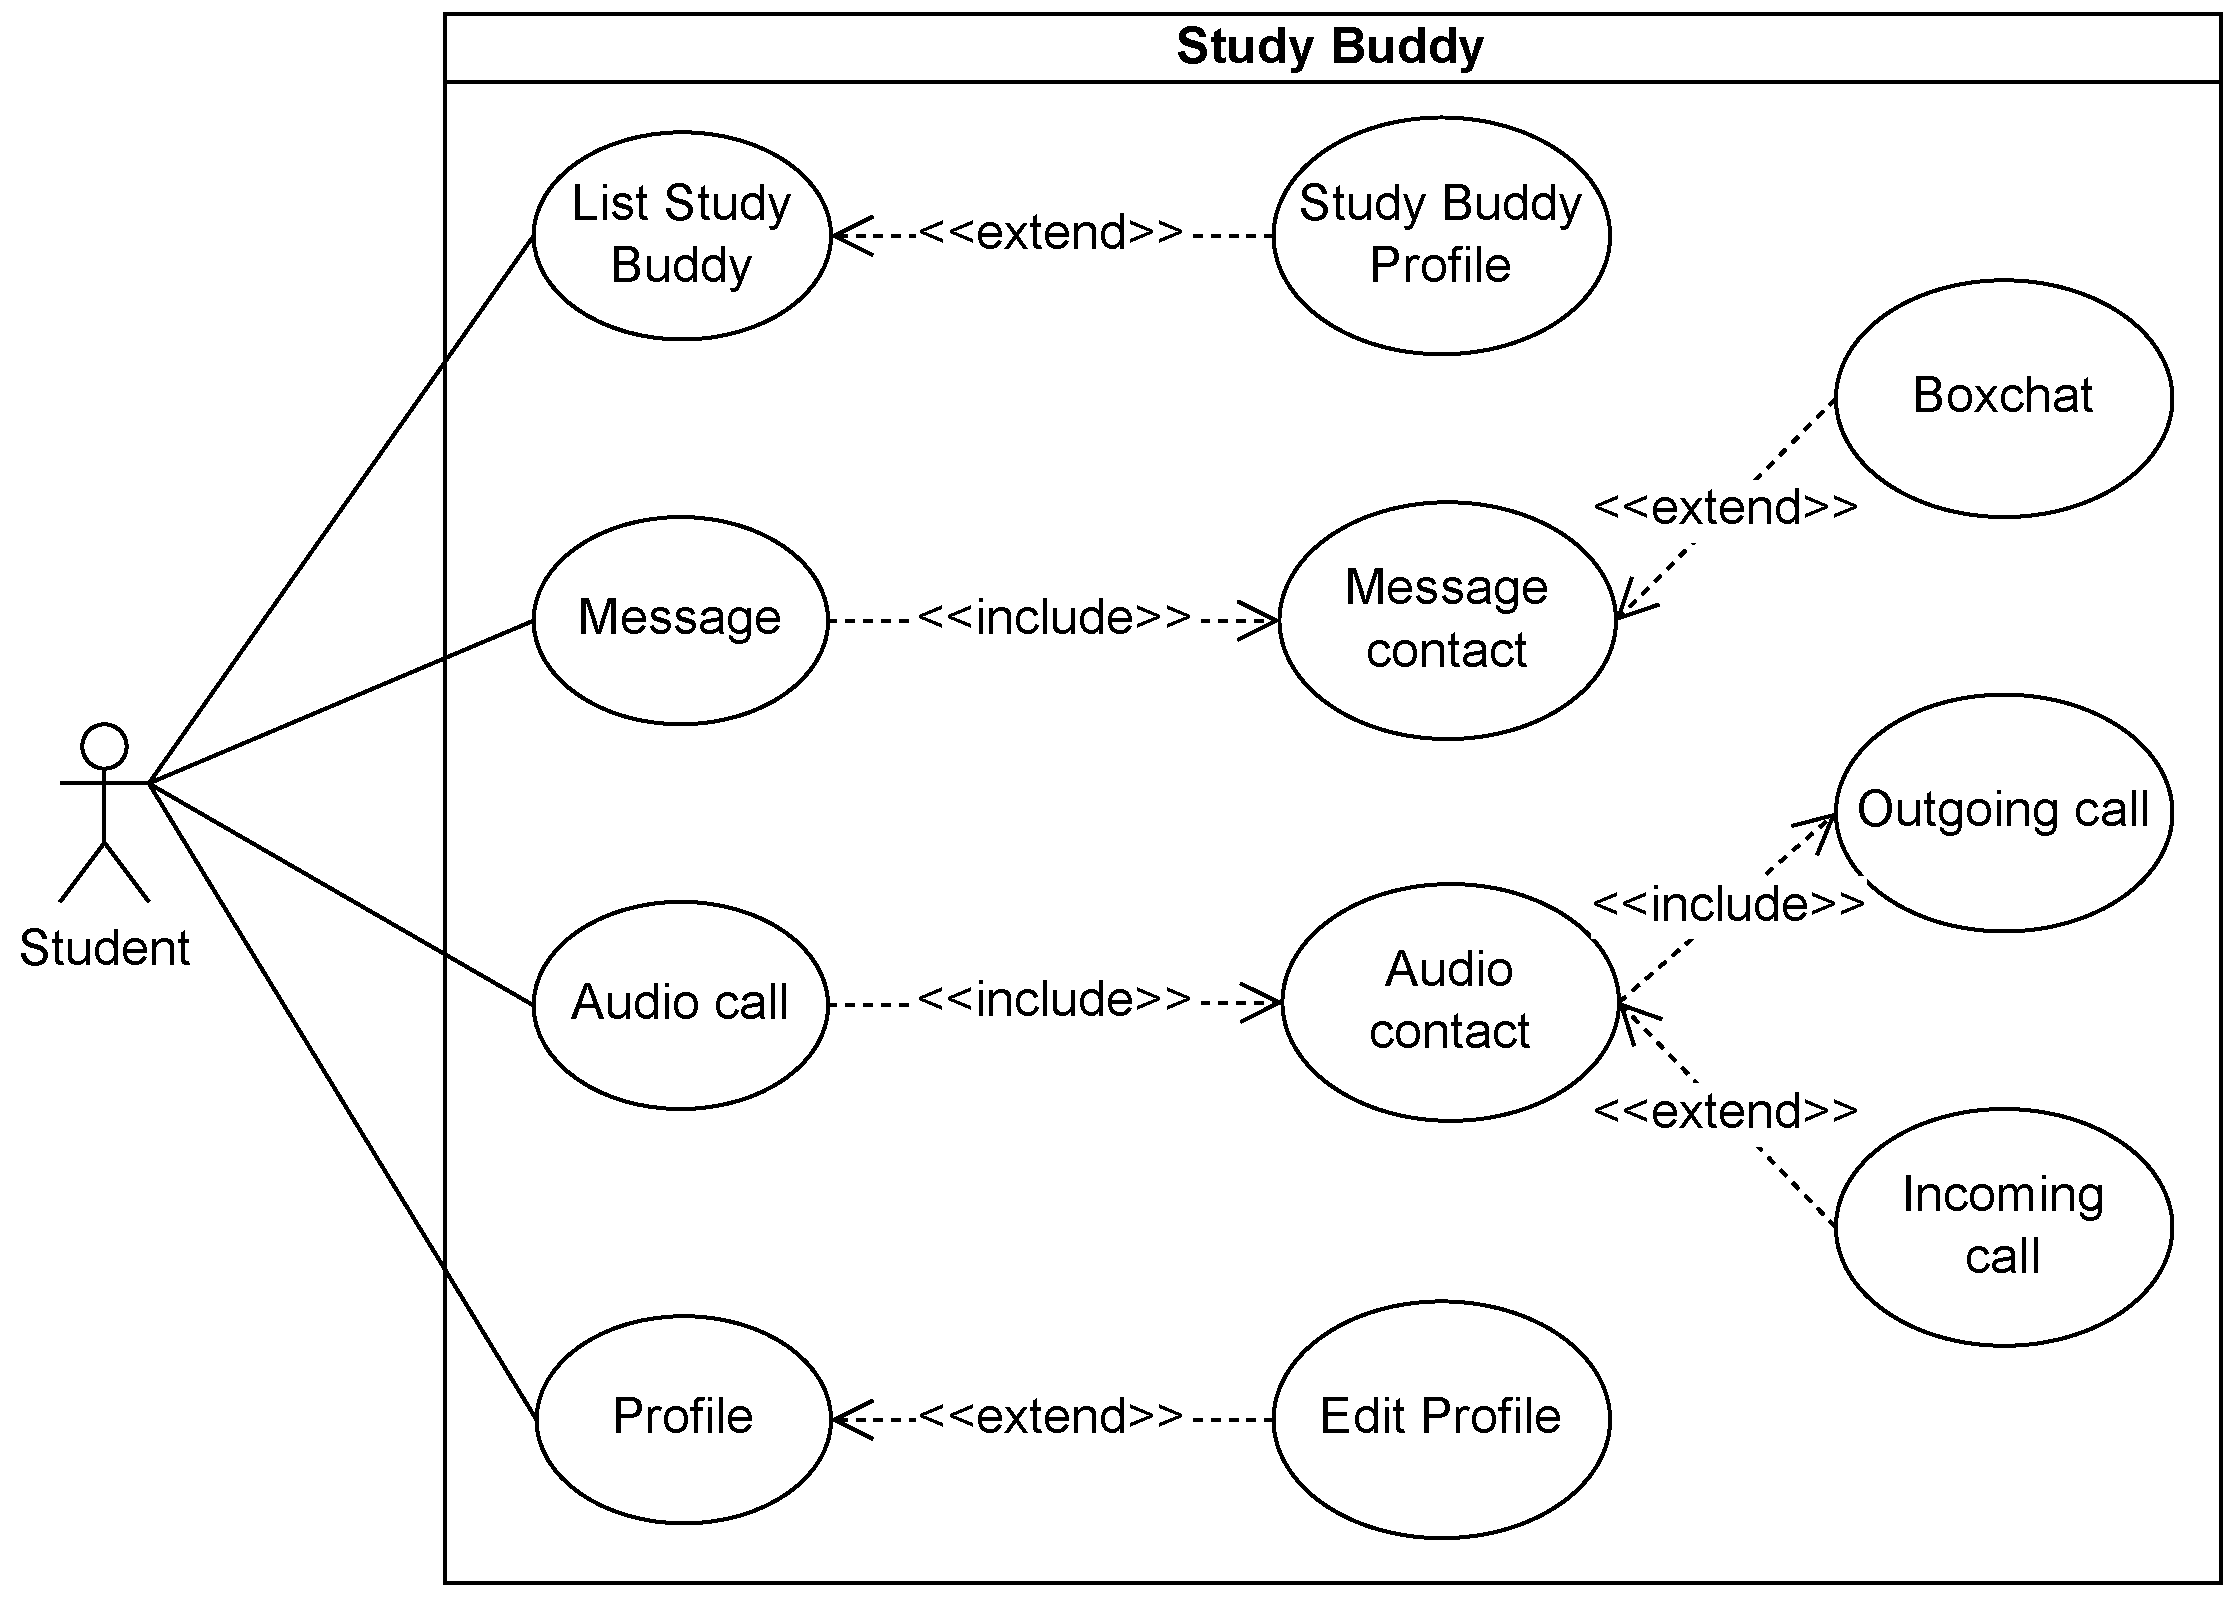
\includegraphics[width=0.7\textwidth]{image/StudyBuddyUseCase.pdf} 
        \caption{StudyBuddy use case diagram}
        \label{fig:studyBuddy_use_case}
    \end{figure}
    \textbf{Description:} The system allows students to connect and find each other students, who have the same things with the other. Students can view their profile, interest, ... \\

    \noindent \textbf{Pre-conditions:} 
        \begin{itemize}
            \item Before this use case begins, students must do a small survey and be logged into the system.
            \item The system must fetch successfully with other students’ profiles.
        \end{itemize}
    \noindent \textbf{Post-conditions:}
    \begin{itemize}
        \item \textbf{Success:}
        \begin{itemize}
            \item User can view a list of suggestion friends; send and receive text message, audio call; view and update profile.
            \item Admins can refresh and reload the suggestion matching list.
        \end{itemize}
        \item \textbf{Failure:}
        \begin{itemize}
            \item The system fails to fetch student data.
            \item System fails to display profile of match recommendation.
            \item System display an error message. 
        \end{itemize}
    \end{itemize}

    \begin{table}[H]
        \centering
        \renewcommand{\arraystretch}{1.5}
        \begin{tabular}{|m{3.5cm}|p{10cm}|} 
            \hline
            \multicolumn{1}{|c|}{\textbf{Actor Action}} & \multicolumn{1}{c|}{\textbf{System Action}} \\ \hline
            \multirow{4}{=}{\centering \shortstack[c]{User click button \\ "StudyBuddy"}} 
            & 1. The system displays a list of Students who are in the list of recommendations \\ \cline{2-2} 
            & 2. After clicking the “Yes” button, add that Student to Chat and Contact \\ \cline{2-2}
            & 3. After clicking the “No” button, remove that Student from the list \\ \cline{2-2}
            & 4. After clicking the “Refresh” button, the system will refresh the list of recommended students \\ \hline
            \multirow{2}{=}{\centering \shortstack[c]{User click button \\ "Message"}} 
            & 1. The system displays students who Students have matched with \\ \cline{2-2}
            & 2. After clicking the box chat, start a chat with another student \\ \hline
            \multirow{2}{=}{\centering \shortstack[c]{User click button \\ "Contact"}} 
            & 1. The system displays students who Students have matched with \\ \cline{2-2}
            & 2. After clicking the contact, start an audio call with another student \\ \hline
            \multirow{2}{=}{\centering \shortstack[c]{User click button \\ "Profile"}} 
            & 1. The system fetches the StudyBuddy profile of Student from the database \\ \cline{2-2}
            & 2. After clicking “Edit Profile”, Students can change information about their StudyBuddy profile after the system is verified \\ \hline
        \end{tabular}
        \caption{Actor Actions and System Actions for StudyBuddy}
        \label{tab:studyBuddy_table}
    \end{table}

\pagebreak

\textbf{Use case: Real Time Notification} \\

    \begin{figure}[H]
        \centering
        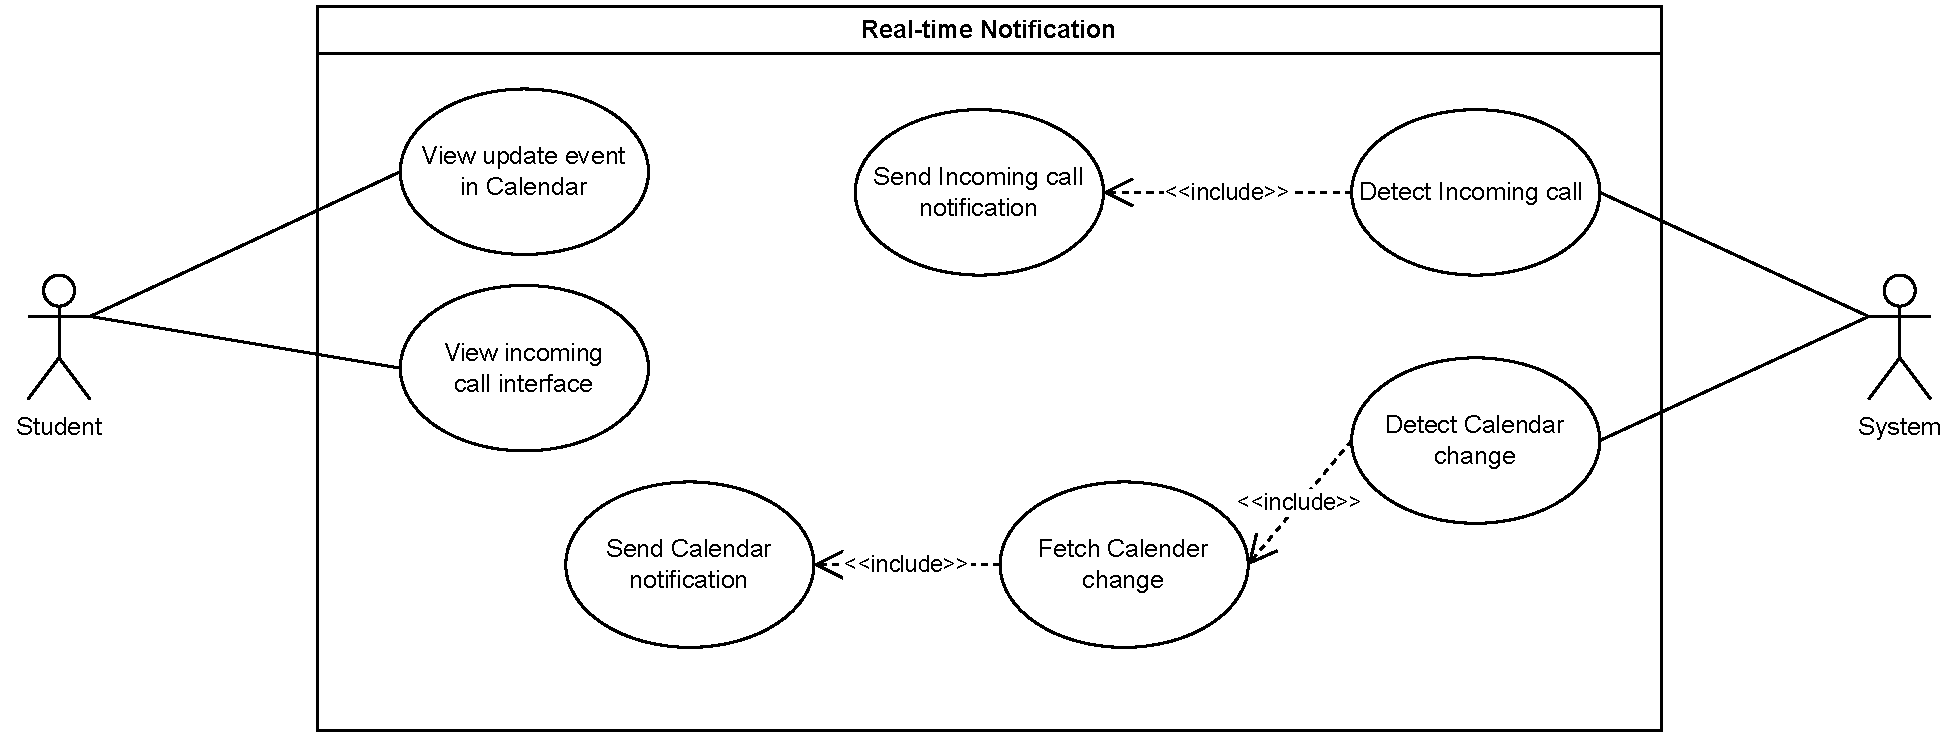
\includegraphics[width=1\textwidth]{image/Real-timeNotificationUseCase.pdf} 
        \caption{Real Time Notification use case diagram}
        \label{fig:notification_usecase}
    \end{figure}
    \textbf{Description:} The push notification system alerts the student whenever there is a change in their calendar (a new event or modification of an existing one) or when they receive a call. Notifications are delivered in real-time, ensuring that the student stays updated on any important events or incoming calls. \\
    
    \noindent \textbf{Pre-conditions:} 
        \begin{itemize}
            \item The user’s device must be connected to the internet.
            \item The student must have granted the application permission to access the calendar and incoming notifications.
        \end{itemize}
    \noindent \textbf{Post-conditions:}
    \begin{itemize}
        \item The real time notification will pop up on the student's device to attract the student's attention.
        \item The notifications will contain:
        \begin{itemize}
            \item A bolded title with context about the notification’s content.
            \item The application icon to show where the notification is coming from.
            \item A subtext for describing more information about the notification.
        \end{itemize}
    \end{itemize}

    \begin{table}[H]
        \centering
        \renewcommand{\arraystretch}{1.5}
        \begin{tabular}{|m{3.5cm}|p{10cm}|} 
            \hline
            \multicolumn{1}{|c|}{\textbf{Actor Action}} & \multicolumn{1}{c|}{\textbf{System Action}} \\ \hline
            \multirow{2}{=}{\centering \shortstack[c]{Admin update or \\ add event to \\ the user’s calendar}} 
            & 1. The system detects the calendar changes and triggers the notification \\
            & \\ \hline 
            \multirow{2}{=}{\centering \shortstack[c]{User receives \\ an incoming call}} 
            & 1. The system identifies incoming calls and sends a push notification to inform users in real time \\ \hline
            \multirow{2}{=}{\centering \shortstack[c]{User click on \\ the notification}} 
            & 1. \textbf{Calendar notification:} The system will open the application and display the updated event on the calendar \\ \cline{2-2}
            & 2. \textbf{Incoming call notification:} The system will open the application and allow the student to handle the incoming call (accept or decline) \\ \hline
        \end{tabular}
        \caption{Actor Actions and System Actions for Real time Notification}
        \label{tab:notification_table}
    \end{table}

\pagebreak

\section{Methodologies}
This section offers an overview of the methodologies used throughout the system development
after examining the objectives of the USTH Connect. It ensures that
essential actions are executed in a systematic and well-planned manner. \\

\subsection{Use Case Implementation}
This section provides an overview of the implementation of use cases in the system, ensuring that
all critical steps are carried out and described in detail.
\subsubsection{Sync Calendar Sequence Diagram}

    \begin{figure}[H]
        \centering
        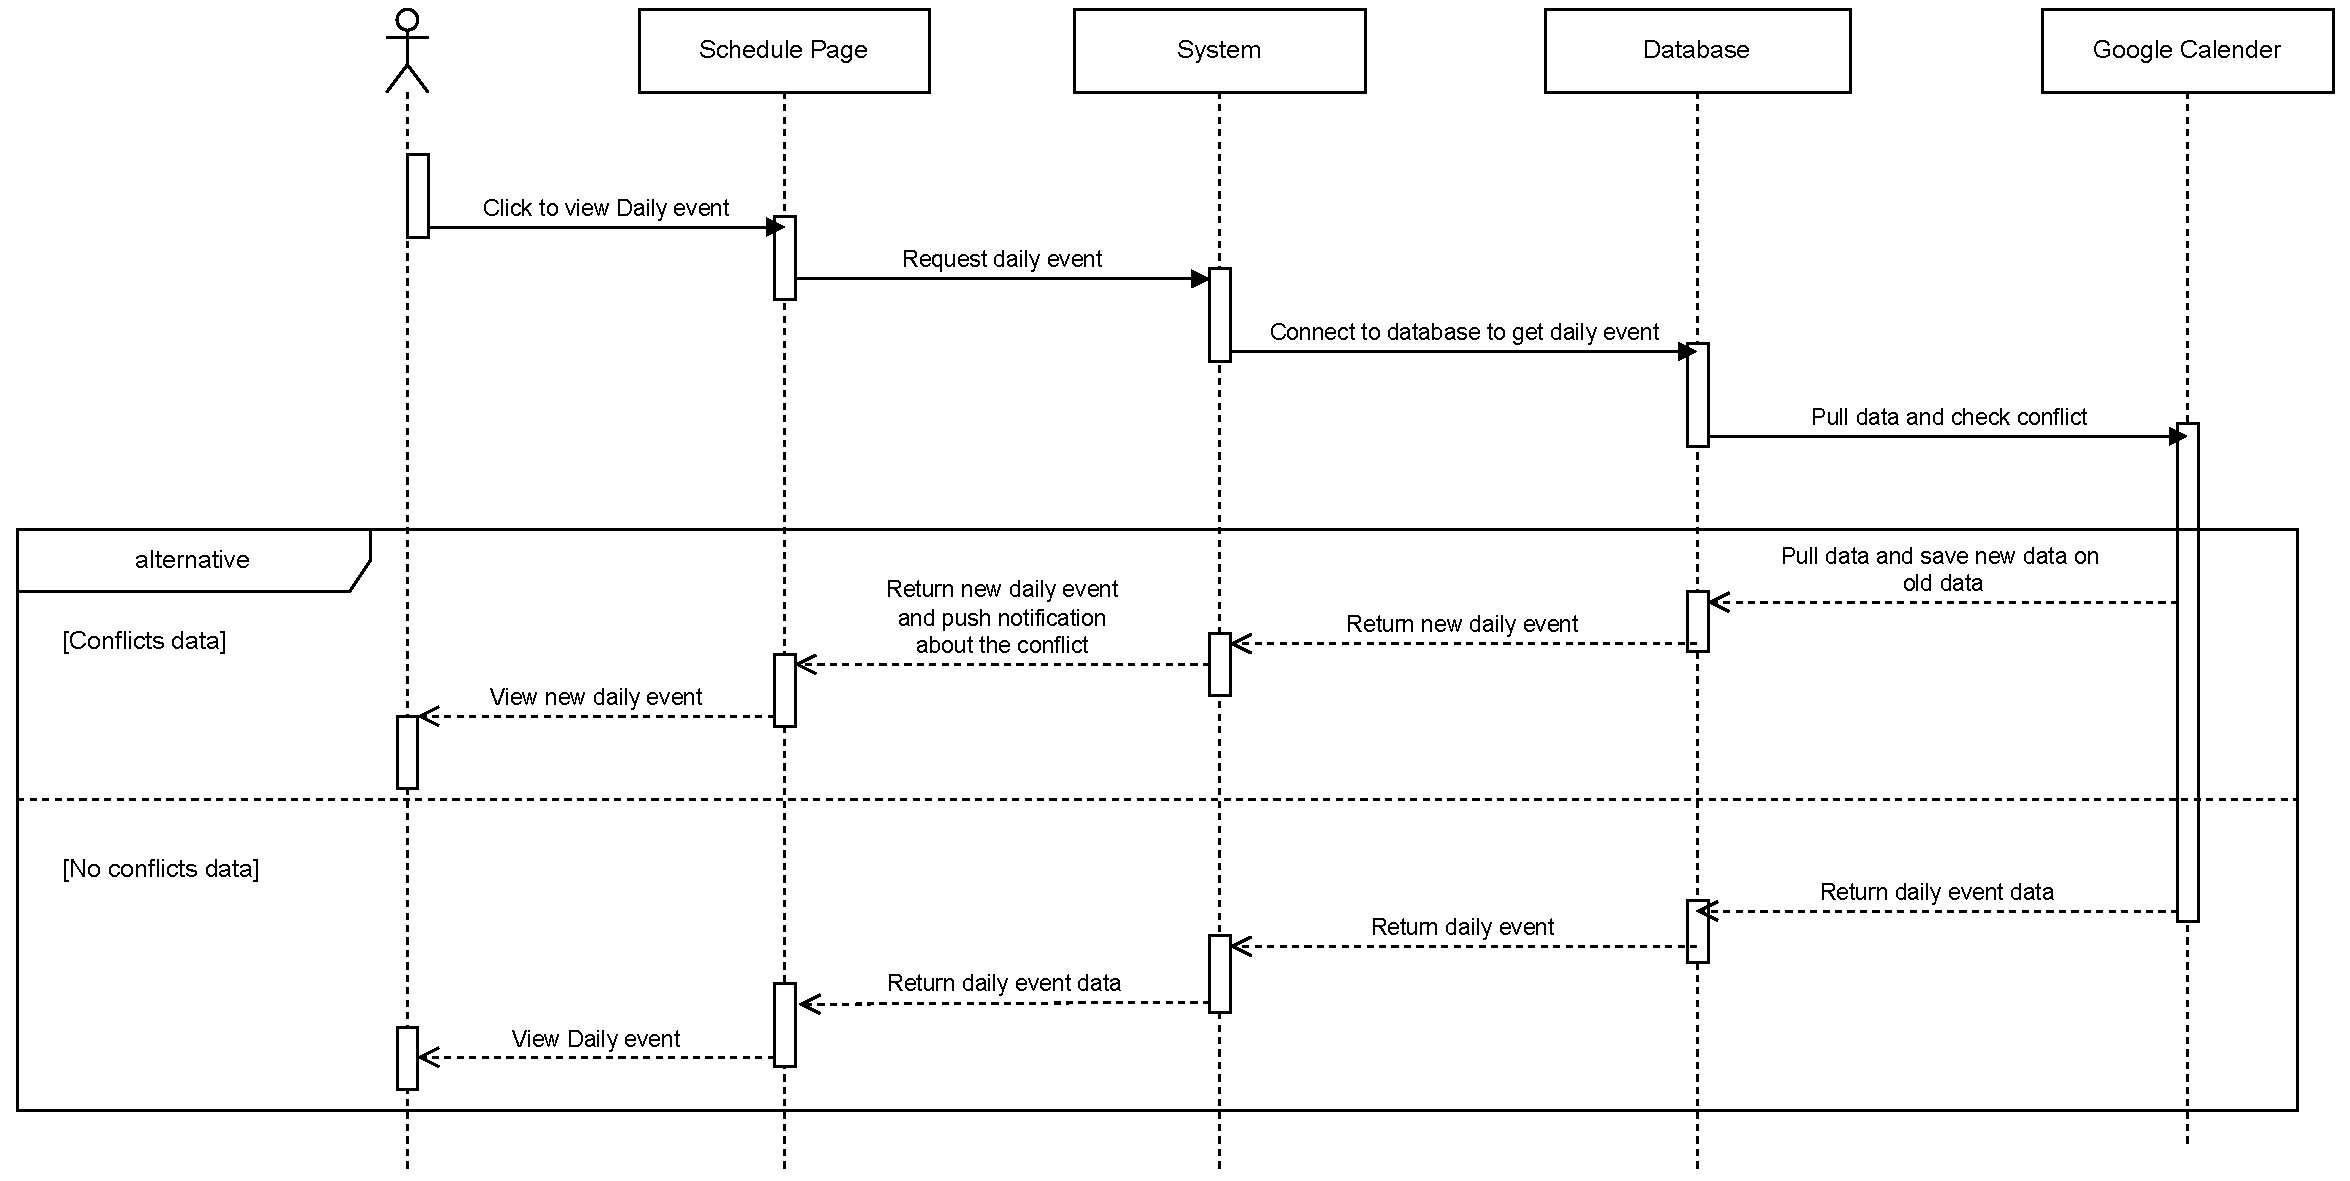
\includegraphics[width=1\textwidth]{image/SyncCalendar.pdf} 
        \caption{Synchronize Calendar sequence diagram}
        \label{fig:sync_calendar_sequence}
    \end{figure}
\subsubsection{Sync Calendar Sequence Diagram}
\begin{figure}[H]
    \centering
    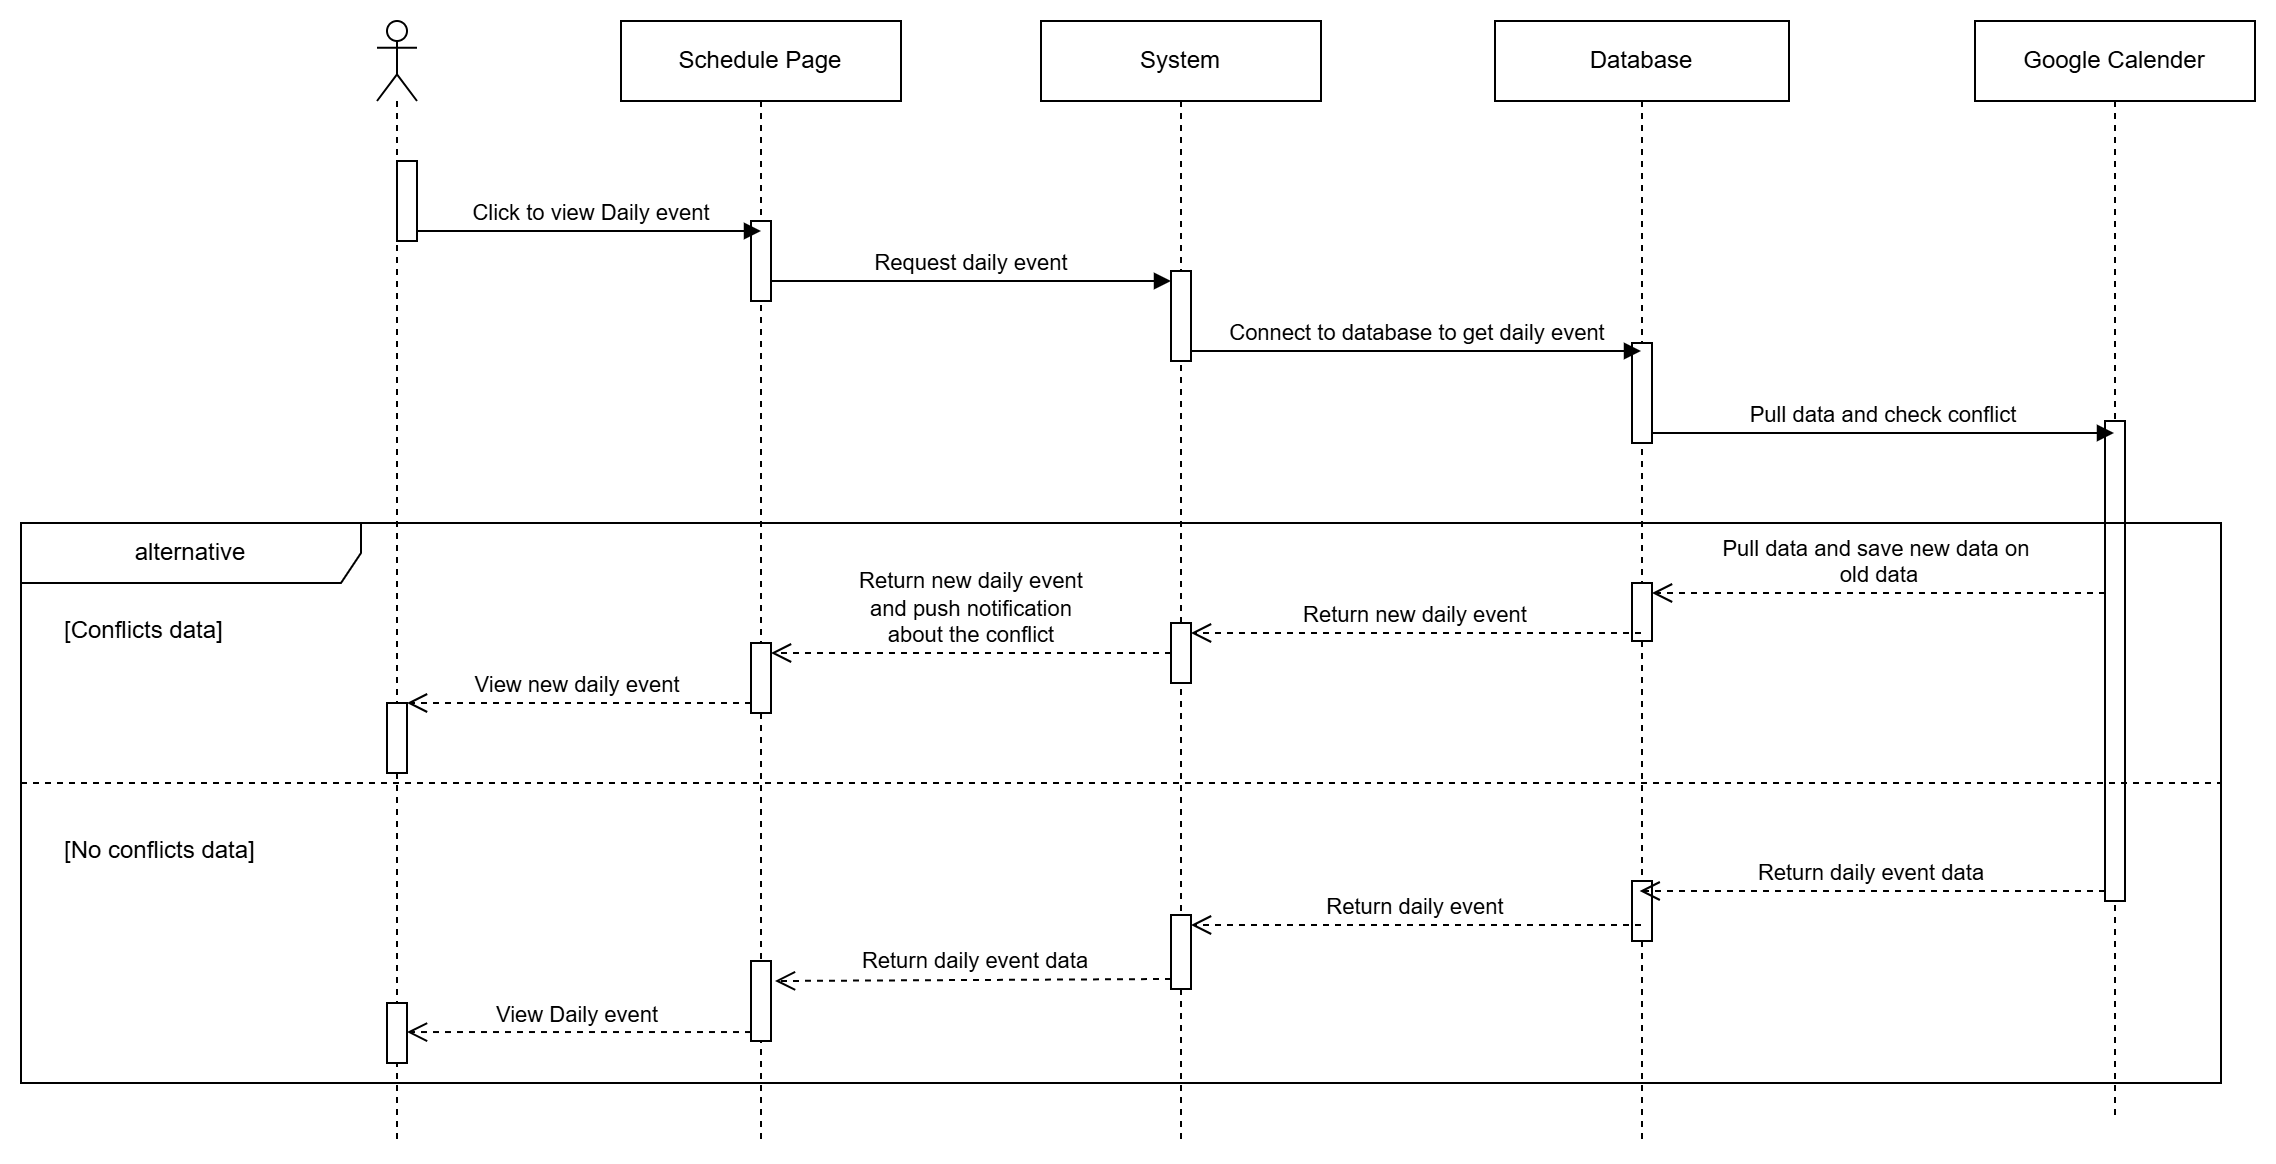
\includegraphics[width=1\textwidth, height=0.3\textheight]{image/SyncCalendar.png} 
    \caption{Synchronize Calendar sequence diagram}
    \label{fig:sync_calendar_sequence}
\end{figure}



\subsubsection{Analysis Call and Message Technologies}
\noindent This section below provides how the contact between users works utilising the help of SIP-based service Linphone.
\subsubsubsection{Session Initiation Protocol}

    In order to facilitate data exchange between two parties, 
    establishing a session is essential. However, identifying and connecting with 
    the second participant can be challenging. To address this, specialized protocols 
    have been designed specifically for such scenarios. \\

    \noindent The Session Initiation Protocol \cite{sip}, 
    commonly known as SIP, is a signaling protocol operating at the 
    application layer, designed for Internet telephony, IP-based telephone systems, 
    as well as mobile phone calling over LTE. SIP’s primary purpose is in VoIP systems, where it serves 
    as a support protocol for registering and locating users, and for call set up and management. It can initiate, maintain, 
    and terminate communication sessions that include voice, video and messaging applications. SIP supports five facets of establishing and terminating multimedia communications: 
    user location, user availability, user capabilities, session setup, and session management. \\

    \noindent SIP functions as a standalone application but relies on other protocols 
    to ensure the overall architecture operates effectively. At the transport layer, 
    it is transported by using the Transmission Control Protocol (TCP), the User Datagram Protocol (UDP), 
    or the Transport Layer Security (TLS) depending on specific circumstances. In this project, 
    TLS is used (more on TLS in Section 1.3). \\

    \noindent SIP architecture consists of:
    \begin{itemize}
        \item \textbf {User Agent (UA):} an end point of the network, able to send requests (also known as User Agent Client - UAC) 
        and receive responses (User Agent Server - UAS). User Agent usually acts as both client and server and some examples 
        are - IP phone, softphone, and camera. The caller’s phone acts as a client and the callee’s phone acts as a server.
        \item \textbf {The Proxy Server:} takes a request from a user agent and forwards it to another user (i.e., an INVITE message).
        \item \textbf {The Registrar Server:} which is responsible for registering users to the network. It accepts registration requests from 
        user agents and helps users to authenticate themselves within the network. It stores the URI and the location of users in a database 
        to help other SIP servers within the same domain.
        \item \textbf {The Redirect Server:} receives requests and looks up the intended recipient of the request in the location database created by the registrar. 
        \item \textbf {The Location Server:} provides information regarding the caller’s possible locations to the Redirect and Proxy Servers.
    \end{itemize}
    \noindent In SIP, Each user is identified with a unique address, called SIP Uniform Resource Identifier (SIP URI). It is an address that contains information for establishing a session with the other end. The SIP URI resembles an E-Mail address and is written in the syntax below with the following URI parameters: 
    SIP - URI = sip:x@y:Port  where x = username and y = host (domain or IP).

\subsubsubsection{Linphone}
    Linphone is an open-source VoIP (Voice over Internet Protocol) application that utilizes SIP-based user agent. VoIP messages and calls are made over an IP network rather than over traditional public switched telephone networks (PSTN). 
    Linphone features all basic SIP-related services, such as audio and video calls, call management, call transfer, audio conferencing, and instant messages. 
    
    \pagebreak

    The free Linphone SIP service is released with an open-source license; and the SIP server software powering this service is called Flexisip. 
    Linphone uses its open-source library as its core, called liblinphone. 
    The library is a SIP-based SDK5 for video and audio over IP and is written in C/C++. 
    The application is available on Linux, Windows, MacOS, iOS, and Android. \\

    \noindent The combination of Linphone and Flexisip SIP proxy provides secure end-user registration and call setup.
    More precisely, Linphone client establishes and maintains a SIP TLS connection to the Flexisip server. 
    The Linphone client verifies the SIP server’s identity based on the X.509 digital certificate of the server (a list of trusted root authorities is provided at compilation time). 
    In this way, message and entity authentication, as well as confidentiality, of the information exchanged between the Linphone client and the Flexisip server is ensured. 
\subsubsubsection{Transport Layer Security Protocol (TLS)}
    Transport Layer Security, or TLS, is a widely adopted security protocol designed to facilitate privacy and data security for communications over the Internet. 
    TLS was derived from a security protocol called Secure Socket Layer (SSL). A primary use case of TLS is encrypting the communication between applications and servers. 
    TLS is based on symmetric encryption and is a client - server model, where the client is able to authenticate the server and, optionally, the server is also able to authenticate the client. \\

    \noindent When using SIP over TLS, the whole SIP signalling is encrypted. However it holds only on the segments of the communication which actually use TLS. 
    Therefore, TLS will be automatically set to each end of the user by default in this project. 


\subsubsubsection{Communication Handling}
\subsubsubsubsection{Call Initialization}
    A session is initiated with an INVITE method which is the request from a UA client (caller). 
    INVITE has attributes containing source address, destination address, and information about the session from the caller. 
    The SIP client creates an INVITE message for callee, which is normally sent to a proxy server.

    \noindent If the OK message takes over 200ms to deliver, the progress and status (TRYING) are sent to the caller. 
    The three-way handshake occurs when the OK message confirms the connection to the caller and the ACK message confirms the existence of connection to the callee. 
    Then the media transport, which is logically separated from session initiation will be established. When there is a BYE message being sent, the session will be terminated. 

    \noindent The most common SIP messages explain for the above figure:
    \begin{itemize}
        \item \textbf {INVITE:} Initiate a dialog for establishing a call. The request is sent by a user agent client to a user agent server.
        \item \textbf {OK:} confirmation of a request.
        \item \textbf {ACK:} confirmation of the connection form caller to callee.
        \item \textbf{BYE:} Signal termination for a session and end a call.
    \end{itemize}

    \noindent Below is the illustration of a simple SIP operations:
    \begin{itemize}
        \item \textbf {Step 1:} SIP client creates INVITE message for callee, which is normally sent to a proxy server. The proxy server will then obtain the IP address of SIP server that handles requests for the requested domain. 
        \item \textbf {Step 2:} The proxy server will reference a location server to identify the next hop server. 
        \item \textbf {Step 3:} The location server (non - SIP server) stores information about the next hop server and will return the IP address of callee.
        \item \textbf {Step 4:} Trying message will be sent to the caller when the session initialization is in process.
        \item \textbf {Step 5:} When the IP address is achieved from the step 3, the proxy server will forward the INVITE message to callee machine.
        \item \textbf {Step 6 and 7:} The callee device will ring and the proxy server will forward the RINGING message from the callee to the caller.
        \item \textbf {Step 8 and 9:} When successfully reaching the callee, if the callee accepts the call, the OK response will be sent back from the callee to the caller through the proxy server.
        \item \textbf {Step 10:} An ACK confirmation will then be sent. After that a full-fledged media session is initiated between UAC and UAS. 
        \item \textbf {Step 11 and 12:} The session will then be terminated when one of two components sends the BYE message. 
    \end{itemize}

    \begin{figure}[H]
        \centering
        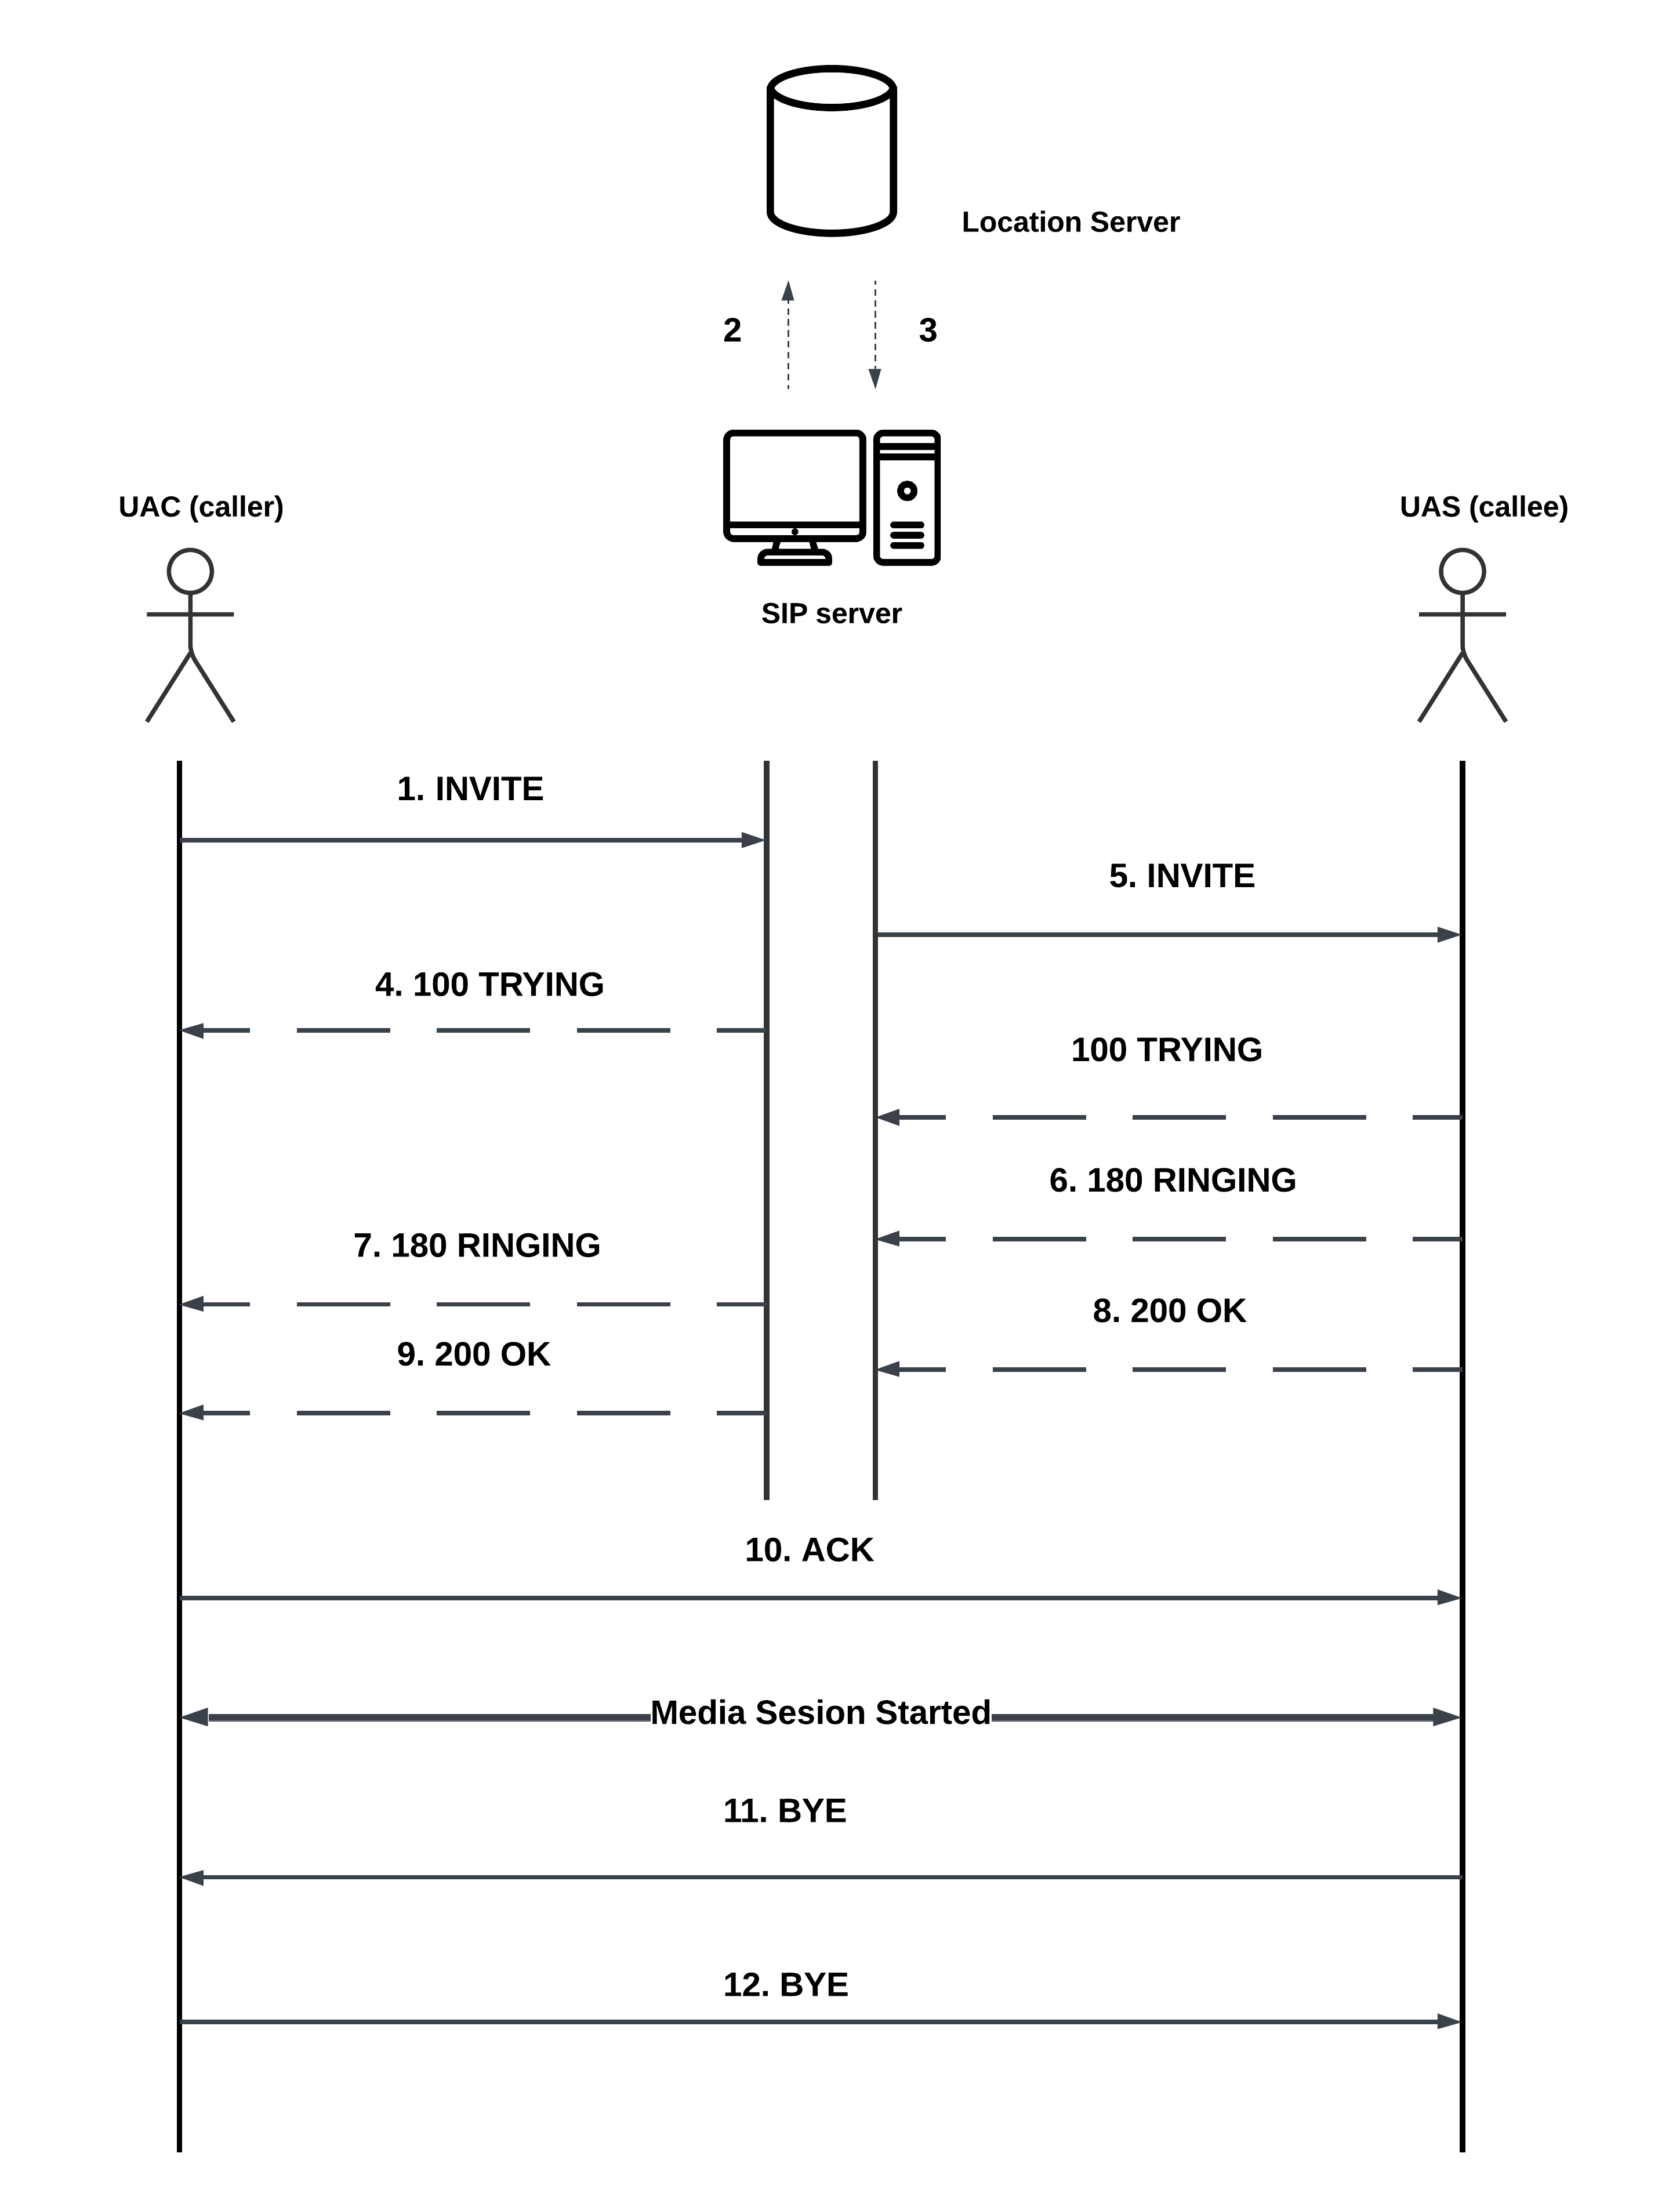
\includegraphics[width=0.7\textwidth]{image/Call Initiation.png} 
        \caption{SIP signaling and key components}
        \label{fig:sip_signaling}
    \end{figure}
    
\subsubsubsubsection{Locating the callee}
    SIP relies on supporting network services like DNS to enable the discovery of proxies and user endpoints. 
    Each user is assigned a unique SIP URI, which is essential for identification and communication. 
    To establish a call using a free SIP service, the following process is typically involved:

    \begin{itemize}
        \item \textbf{Account Registration:} A user registers an account with the free SIP service, which provides a unique SIP URI (e.g., sip: username@sip.linphone.org). 
        This registration associates the user with a proxy server, making them reachable for SIP signaling.
        \item \textbf{Call Setup:} To initiate a call, the SIP client uses the provided SIP URI and sends an INVITE message to the proxy server. 
        The proxy server relies on DNS to locate the callee's proxy server and forwards the INVITE message accordingly.
        \item \textbf{DNS Role in Call Routing:} DNS resolves the domain portion of the SIP URI (e.g., sipserver.com) to the corresponding SIP server's IP address. 
        This process ensures that the caller's proxy server can locate the appropriate next-hop server to route the call.
        \item \textbf{Communication Establishment:}  Once the proxy servers successfully exchange SIP signaling messages, the callee's user agent receives the call request, and the session is established.
    \end{itemize}

    \noindent The figure below shows the SIP registration process and how to detect the location of the callee. 
    \sloppy
    \begin{itemize}
        \item \textbf {Step 1:} One user agent with SIP URI \texttt{sip:callee\_username@sip.linphone.org} register to linphone free sip service registrar server. 
        This server stores the user’s URI and current IP address in its location service database. 
        This makes sure that the user is reachable within the \texttt{sip.linphone.org} domain. 
        \item \textbf {Step 2:} Linphone’s registrar updates its location service with the association of \texttt{sip:\allowbreak callee\_username@sip.linphone.org}.
        \item \textbf {Step 3:} Another user agent (the caller), with the SIP URI \texttt{\allowbreak sip:caller\_username\allowbreak @sip.linphone.org}, 
        sends an INVITE message to their local proxy server. 
        The destination address in the INVITE is \texttt{sip:caller\_username@sip.linphone.org}.
        \item \textbf {Step 4 and 5:} The SIP server will then query for its location service and receive the register address of the callee user agent.
        \item \textbf {Step 6:} The proxy server will then forward the INVITE method to the callee’s device. 
    \end{itemize}

    \begin{figure}[H]
        \centering
        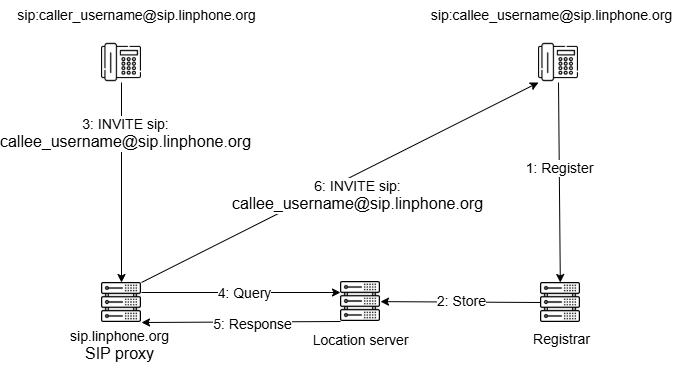
\includegraphics[width=0.7\textwidth]{image/Locating_calllee.png} 
        \caption{SIP registration and locating callee}
        \label{fig:locating_callee}
    \end{figure}

\subsubsubsubsection{One-on-One Instant Messaging}
    Instant Messaging is the process of transfering of messages between users in near real-time.
    The back and forth process to transfer messages have to be fast enough for participants to sustain an interactive dialogue.
    MESSAGE method - an extension to SIP is used to deliver messages between users. 

    \noindent The user must login using the correct right credentials (username and password), that informations will then be send to the Flexisip server of Linphone.
    The Flexisip server will then create a temporary file which includes user contact list information 

\subsection{System Architecture}
This section provides an overview of the technologies and components used in the system.
It focuses on the roles and interactions of various systems and services that work together in a layered architecture with a client-server relation, creating a seamless, integrated solution for university life assistance and student networking.

\subsubsection{System Architecture Diagram}
\begin{figure}[H]
    \centering
    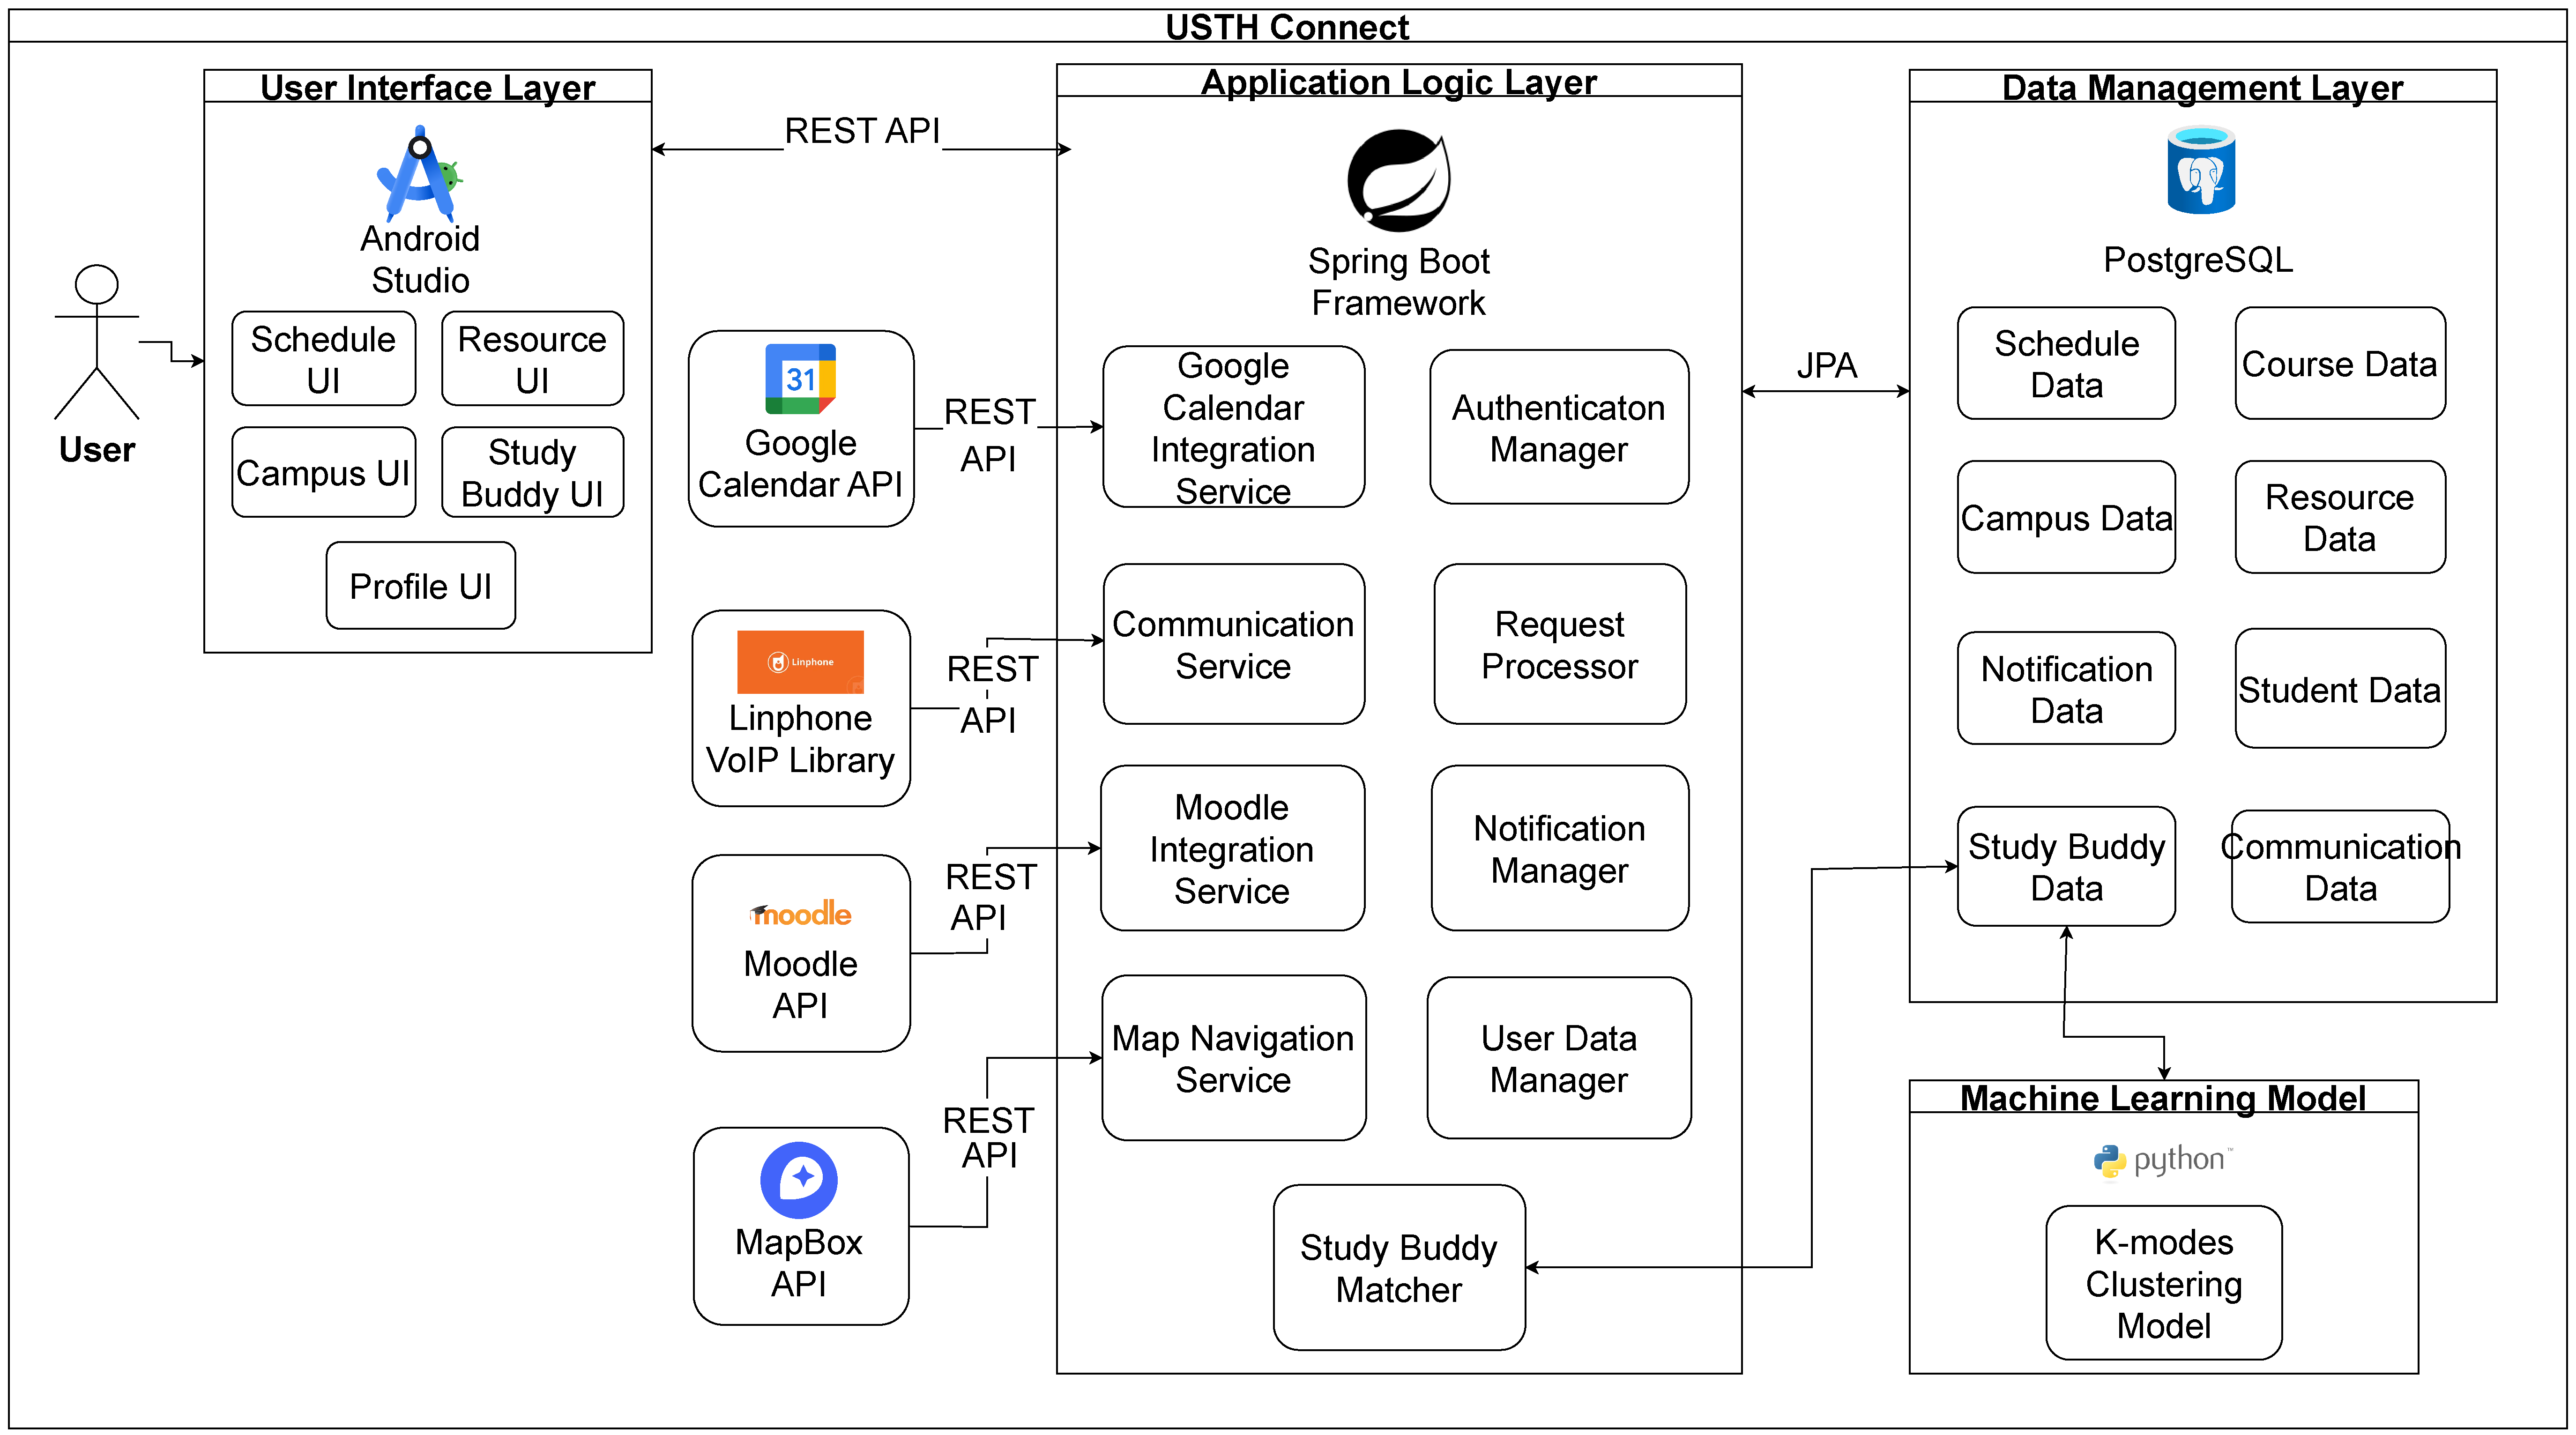
\includegraphics[width=\textwidth]{image/System_Architecture_USTH_Connect.pdf} 
    \caption{USTH Connect System Architecture Diagram}
\end{figure}

\pagebreak

\subsubsection{Backend - Spring Boot}
The backend of the application is configured using Spring Boot, a well-known and powerful Java framework for its ability to simplify the backend development.
Spring Boot handles the core logic of the application, which includes student authentication, processing data from third-party services, and providing APIs for the mobile frontend.
It configures a seemless integration with various services such as Google Calendar, Mapbox, and Moodle, ensuring that schedule events, campus locations, and lecture resouces are always up-to-date and easy to access.
The backend is responsible for processing and storing student data, managing roles with JWT for secure access, and applying RBAC to differentiate between ADMIN and USER roles.
This security configuration ensures that students can only access the data and features which are allowed according to their given roles, enhancing the security and functionality of the system.

\subsubsection{Mobile Frontend - Java (Android)}
The mobile app is developed using Java for Android, which acts as the UI for the system.
This frontend enables students to interact with various features, such as viewing events from Google Calendar, accessing campus location through Mapbox, and browsing academic resources coming from Moodle.
The app fetches data from the backend through APIs, ensuring that it always displays the latest information that the backend system can provide.
For the Google Calendar implementation, the app periodically retrieves and displays these followings events, which makes it easier for students to stay updated on their study schedules.
Mapbox provides an overview map of a campus, allowing students to locate buildings and study halls using their latitude and longitude data.
Additionally, the app integrates the StudyBuddy feature, where students can find potential study partners based on their personal description, interests and habits. 
Moreover, it supports real-time audio and message communication through the Linphone VoIP library. \\

The frontend UI service is necessary in our system architecture because it acts as the bridge between the user and the system's backend service. The UI provides students with an user-friendly interface to access the application features such as schedule view, campus navigation, resource access, and academic collboration.
Without the frontend UI, the system would lack a method for students to communicate to the backend service, therefore the application is considered unusable. 
The frontend ensures that the students have a smooth and comfortable experience while using our platform, which helps them improving their academic life and connecting with their peers seamlessly.

\pagebreak

\pagebreak

\subsubsection{Machine Learning - K-modes Clustering}
The StudyBuddy feature of the system using a Python-based machine learning model that uses the K-modes clusteting algorithm to match students based on their personal interests and study preferences.
When students enter details about their personality traits, hobbies, learning style and academic goals, this data is sent to the backend, which processes it using the K-modes algorithm.
After receiving data, the algorithm groups students with similar characteristics, enabling the system to send back the proper recommendation to the students.
Then, the potential study partners will be displayed in the mobile app, allowing students to connect to each others who have compatible interests.
This feature is implemented using Python's machine learning libraries, which provide the necessary methods for clustering and pattern recognition in student matching. \\

There are many advantages for why Python was chosen over Java for the implementation of the machine learning model in our system architecture. First, the libraries which are designed specifically for machine learning configuration are offered by Python, such as (Add used libraries). These libraries provide powerful and optimized tools for implementing our algorithm which is K-modes clustering, fostering faster development and experimentation.
Regarding Java, it lacks various of tools which directly support the implementation process and require more complex and custom implementations. Additionally, Python provides direct support for the K-modes clustering algorithm through the kmodes library, which is a key reason why we choose Python over Java in the implementation of the machine learning model.
As regards to the process of prototyping and experimentation, which is significant for fine-tuning machine learning models, Python allows a faster and short duration for this process. Finally, Python integrates seamlessly with the backend services, ensuring easy communication with other system components through APIs.
In conclusion, Python is considered as the most suitable choice for implementing the required machine Learning model which plays a crucial role in the StudyBuddy feature.

\subsubsection{Communication - Linphone VoIP}
To integrate real-time communication between matched students, the system implements Linphone, an open-source VoIP library.
Linphone allows students to initiate audio calls, enabling seamless communication for students who wish a collaboration on projects or study-together session.
After the StudyBuddy algorithm matches two studens, they can contact and communicate each other through the app through the app using the Linphone VoIP integration.
Therefore, that students can interact with their matches without relying on external messaging or calling services.
Linphone provides a reliable and efficient platform for voice communication, contributing to the goal of encouraging more interaction and collaboration between students in the university.

\subsubsection{How Does The System Work?}
This system combines multiple components to work well together.
The Spring Boot backend serves as the brain of the operation, managing user accounts, data storage, and communication with external services like Google Calendar, Mapbox, Moodle, and Linphone VoIP library.
The mobile app, built with Java, communicates with the backend to access real-time information. To connect students with similar interests, the system employs a smart matching algorithm (using Python). 
Once matched, students can easily make voice calls within the app thanks to Linphone's built-in calling feature. \\

The mobile app uses REST APIs to send requests to the backend and receive responses for features like schedules, campus navigation, learning material, and StudyBuddy matches. 
The backend connects to the PostgreSQL databases through JPA, which simplifies database interaction by using ORM.
This allows the backend to retrieve, update, and store data, such as user profiles, schedules, and course materials, through entities and repositories.
When necessary, the backend also interacts with external services like Google Calendar, MapBox, Moodle, and Linphone VoIP through their APIs to fetch or synchronize required information.
This structured communication ensures all components can work together, provide accurate and real-time data to the users.\\

The mobile app depends on the backend for up-to-date information, while the backend uses the database and external services to ensure smooth operations.
In summary, this system provides students with a comprehensive platform that support their academic needs and encourages better communication and collaboration.

\pagebreak
\subsection{Database Design}
This section provides a detailed description of the database design for the USTH Connect application.
It highlights the key requirements, objectives, and the structure that support the system's functionality.
Each table and its relationships are thoroughly designed to handle different types of data, such as student profiles, schedule events, course resources, campus naviation, and StudyBuddy connections.
This section also includes an Entity-Relationship diagram that visually represents the relationships between various entities.

\subsubsection{Database Requirements and Objectives}  
The database for USTH Connect is designed to manage a wide range of information, including student profiles, schedules, study buddy connections, and course resources. The main objectives of the database design are:  
\begin{itemize}  
    \item To provide a reliable and centralized system for storing academic and social data.  
    \item To ensure data integrity and maintain relationships between tables for accurate reporting and queries.  
    \item To support seamless integration with external services, such as Google Calendar and Moodle.  
    \item To enable efficient data retrieval for features like StudyBuddy matching, schedule updates, and resource access.  
    \item To maintain scalability and adaptability for increasing student data as the system grows.  
\end{itemize} 

\subsubsection{Entity-Relationship Diagram}
\newgeometry{top=0cm, bottom=0cm, left=0cm, right=0cm} 
\begin{figure}[H]
    \centering
    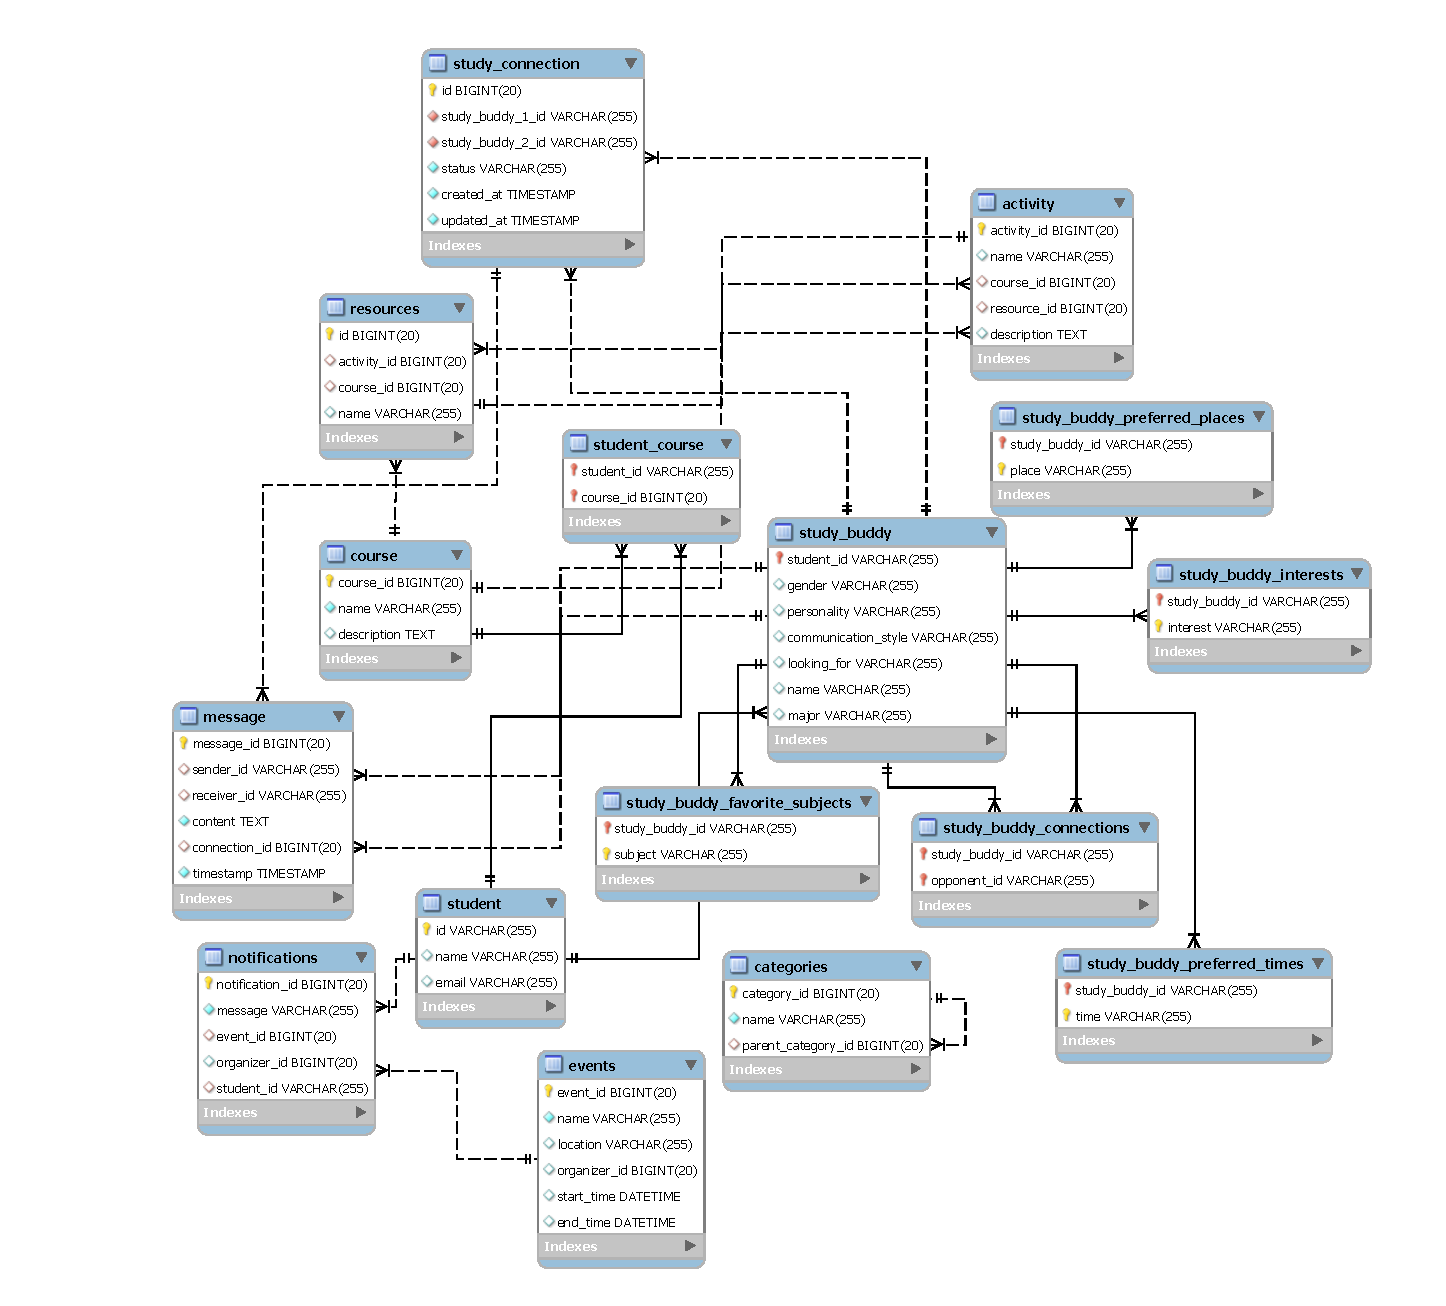
\includegraphics[width=\paperwidth,height=\paperheight,keepaspectratio]{image/USTH-Connect-Database-Schema-v1-cropped.pdf}
\end{figure}
\restoregeometry

\subsubsection{Table and Relationships}
This section provides a detailed description of the tables within the USTH Connect database and their relationship. \\

\textbf{Table: Activity} \\

\textbf{Attributes and Data Types}
\begin{table}[H]
    \centering
    \renewcommand{\arraystretch}{1.5}
    \begin{tabular}{|l|l|p{4.5cm}|l|}
    \hline
    \rowcolor[HTML]{96FFFB} 
    \textbf{Column Name} & \textbf{Data type}      & \textbf{Description}                          & \textbf{Constraints}  \\ \hline
    activity\_id         & bigserial               & Unique identifier for the activity            & Primary Key, Not Null \\ \hline
    activity\_name       & varchar(255)            & Name of the activity                          &                       \\ \hline
    activity\_type       & varchar(255)            & Type of activity                              &                       \\ \hline
    due\_date            & timestamp               & Deadline for the activity                     &                       \\ \hline
    completion\_status   & varchar(255)            & Status of the activity                        &                       \\ \hline
    course\_id           & bigint                  & ID of the course associated with the activity & Foreign Key           \\ \hline
    resource\_id         & bigint                  & ID of a resource associated with the activity & Foreign Key           \\ \hline
    \end{tabular}
    \caption{Attributes and data types for the \texttt{Activity} table}
\end{table}

\noindent
\textbf{Constraints}
\begin{itemize}
    \item \textbf{Primary Key}: \texttt{activity\_id}
    \item \textbf{Foreign Key (\texttt{course\_id})}: References \texttt{course(course\_id)}.
    \item \textbf{Foreign Key (\texttt{resource\_id})}: References \texttt{resources(id)}.
\end{itemize}

\noindent
\textbf{Relationships}
\begin{itemize}
    \item Each \texttt{activity} belongs to one \texttt{course}.
    \item Each \texttt{activity} may have one associated \texttt{resource}.
\end{itemize}

\pagebreak

\textbf{Table: Course} \\

\textbf{Attributes and Data Types}
\begin{table}[H]
    \centering
    \renewcommand{\arraystretch}{1.5}
    \begin{tabular}{|l|l|p{4.5cm}|l|}
    \hline
    \rowcolor[HTML]{96FFFB} 
    \textbf{Column Name} & \textbf{Data type} & \textbf{Description}                        & \textbf{Constraints}  \\ \hline
    course\_id           & bigserial          & Unique identifier for the course            & Primary Key, Not Null \\ \hline
    short\_name          & varchar(255)       & Short Name of the course                    & Not Null              \\ \hline
    full\_name           & varchar(255)       & Full Name of the course                     & Not Null              \\ \hline
    description          & varchar(255)       & Description of the course                   &                       \\ \hline
    visibility           & boolean            & The current visibility status of the course &                       \\ \hline
    \end{tabular}
    \caption{Attributes and data types for the \texttt{Course} table}
\end{table}

\noindent
\textbf{Constraints}
\begin{itemize}
    \item \textbf{Primary Key}: \texttt{course\_id}
    \item \textbf{Foreign Key (\texttt{course\_id})}: In the \texttt{student\_course} table, \texttt{course\_id} references \texttt{course(course\_id)}.
\end{itemize}

\noindent
\textbf{Relationships} 
\begin{itemize}
    \item Each \texttt{course} can be associated with multiple \texttt{students} through the \texttt{student\_course} table.
\end{itemize}

\pagebreak

\textbf{Table: Events} \\

\textbf{Attributes and Data Types}
\begin{table}[H]
    \centering
    \renewcommand{\arraystretch}{1.5}
    \begin{tabular}{|l|l|p{4.5cm}|l|}
    \hline
    \rowcolor[HTML]{96FFFB} 
    \textbf{Column Name} & \textbf{Data type} & \textbf{Description}                      & \textbf{Constraints}  \\ \hline
    event\_id            & serial             & Unique identifier for the events          & Primary Key, Not Null \\ \hline
    event\_name          & text               & Name of the event                         &                       \\ \hline
    event\_description   & text               & Description of the event                  &                       \\ \hline
    event\_start         & timestamp          & Starting time of the event                &                       \\ \hline
    event\_end           & timestamp          & Ending time of the event                  &                       \\ \hline
    location             & varchar(255)       & Location of the Event                     &                       \\ \hline
    organizer\_id        & int                & Unique identifier for the organizer       &                       \\ \hline
    google\_event\_id    & varchar(255)       & Unique identifier generated by the google &                       \\ \hline
    \end{tabular}
    \caption{Attributes and data types for the \texttt{Events} table}
\end{table}

\noindent
\textbf{Constraints}
\begin{itemize}
    \item \textbf{Primary Key}: \texttt{event\_id}.
    \item \textbf{Foreign Key (\texttt{organizer\_id})}: References \texttt{organizer(id)}.
    \item \textbf{Unique Key (\texttt{google\_event\_id})}: Ensures uniqueness of the Google Event ID.
\end{itemize}


\noindent
\textbf{Relationships} 
\begin{itemize}
    \item Each \texttt{event} is organized by one \texttt{organizer}.
    \item Each \texttt{event} is associated with one \texttt{location} from \texttt{maps}.
\end{itemize}

\pagebreak
\textbf{Table: Maps} \\

\textbf{Attributes and Data Types}
\begin{table}[H]
    \centering
    \renewcommand{\arraystretch}{1.5}
    \begin{tabular}{|l|l|p{2.1cm}|l|}
    \hline
    \rowcolor[HTML]{96FFFB} 
    \textbf{Column Name} & \textbf{Data type} & \textbf{Description}                   & \textbf{Constraints}            \\ \hline
    id                   & serial             & Unique identifier for the map location & Primary Key, Not Null           \\ \hline
    location             & varchar(255)       & The name of the location               & Default: "No Location Provided" \\ \hline
    location\_value      & varchar(255)       & Value the location                     &                                 \\ \hline
    Latitude             & double precision   & Latitude of the location               &                                 \\ \hline
    Longitude            & double precision   & Longitude of the location              &                                 \\ \hline
    \end{tabular}
    \caption{Attributes and data types for the \texttt{Maps} table}
\end{table}

\noindent
\textbf{Constraints}
\begin{itemize}
    \item \textbf{Primary Key}: \texttt{id}.
    \item \textbf{Unique Key}: \texttt{location}.
\end{itemize}

\noindent
\textbf{Relationships} 
\begin{itemize}
    \item Each \texttt{location} in \texttt{maps} can be referenced in \texttt{events}.
\end{itemize}

\pagebreak

\textbf{Table: Message} \\

\textbf{Attributes and Data Types}
\begin{table}[H]
    \centering
    \renewcommand{\arraystretch}{1.5}
    \begin{tabular}{|l|l|p{4.5cm}|l|}
    \hline
    \rowcolor[HTML]{96FFFB} 
    \textbf{Column Name} & \textbf{Data type}        & \textbf{Description}                                   & \textbf{Constraints}             \\ \hline
    id                   & bigserial               & Unique identifier for the message                     & Primary Key, Not Null            \\ \hline
    connection\_id       & bigint                  & Reference to the connection in the \texttt{Study Connection} table & Foreign Key, Not Null           \\ \hline
    sender\_id           & varchar(255)            & Identifier of the sender                              & Foreign Key, Not Null            \\ \hline
    receiver\_id         & varchar(255)            & Identifier of the receiver                            & Foreign Key, Not Null            \\ \hline
    content              & varchar(255)            & Text content of the message                           & Not Null                         \\ \hline
    created\_at          & timestamp               & Timestamp when the message was created                & Not Null, Default: \texttt{now()} \\ \hline
    is\_read             & boolean                 & Indicates if the message has been read                & Not Null, Default: \texttt{false} \\ \hline
    \end{tabular}
    \caption{Attributes and data types for the \texttt{Message} table}
\end{table}

\noindent
\textbf{Constraints}
\begin{itemize}
    \item \textbf{Primary Key}: \texttt{id}.
    \item \textbf{Foreign Key}: 
    \begin{itemize}
        \item \texttt{connection\_id} references \texttt{id} in the \texttt{Study Connection} table, with \texttt{ON DELETE NO ACTION}.
        \item \texttt{receiver\_id} references \texttt{student\_id} in the \texttt{Study Buddy} table, with \texttt{ON DELETE NO ACTION}.
        \item \texttt{sender\_id} references \texttt{student\_id} in the \texttt{Study Buddy} table, with \texttt{ON DELETE NO ACTION}.
    \end{itemize}
\end{itemize}

\noindent
\textbf{Indices}
\begin{itemize}
    \item \texttt{idx\_connection\_id}: Index on \texttt{connection\_id} for optimized query performance.
    \item \texttt{idx\_receiver\_id}: Index on \texttt{receiver\_id} for optimized query performance.
    \item \texttt{idx\_sender\_id}: Index on \texttt{sender\_id} for optimized query performance.
\end{itemize}

\pagebreak

\noindent
\textbf{Relationships} 
\begin{itemize}
    \item Each \texttt{Message} is associated with a specific \texttt{Connection}.
    \item \texttt{sender\_id} and \texttt{receiver\_id} reference students in the \texttt{Study Buddy} table.
\end{itemize}


\textbf{Table: Notifications} \\

\textbf{Attributes and Data Types}
\begin{table}[H]
    \centering
    \renewcommand{\arraystretch}{1.5}
    \begin{tabular}{|l|l|p{2.1cm}|l|}
    \hline
    \rowcolor[HTML]{96FFFB} 
    \textbf{Column Name} & \textbf{Data type}        & \textbf{Description}                                   & \textbf{Constraints}             \\ \hline
    notification\_id     & serial                  & Unique identifier for the notification                & Primary Key, Not Null            \\ \hline
    student\_id          & varchar(255)            & Identifier of the student receiving the notification   & Foreign Key, Not Null            \\ \hline
    message              & text                    & The content of the notification                       & Not Null                         \\ \hline
    created\_at          & timestamp               & Timestamp when the notification was created            & Not Null, Default: \texttt{CURRENT\_TIMESTAMP} \\ \hline
    is\_read             & boolean                 & Indicates if the notification has been read            & Not Null, Default: \texttt{false} \\ \hline
    event\_id            & integer                 & Reference to the event related to the notification    & Foreign Key                      \\ \hline
    organizer\_id        & integer                 & Reference to the organizer of the event               & Foreign Key                      \\ \hline
    \end{tabular}
    \caption{Attributes and data types for the \texttt{Notifications} table}
\end{table}

\pagebreak

\noindent
\textbf{Constraints}
\begin{itemize}
    \item \textbf{Primary Key}: \texttt{notification\_id}.

    \item \textbf{Foreign Key}: 
    \begin{itemize}
        \item \texttt{student\_id} references \texttt{id} in the \texttt{Student} table, with \texttt{ON DELETE NO ACTION}.
        \item \texttt{event\_id} references \texttt{event\_id} in the \texttt{Events} table, with \texttt{ON DELETE NO ACTION}.
        \item \texttt{organizer\_id} references \texttt{id} in the \texttt{Organizers} table, with \texttt{ON DELETE NO ACTION}.
    \end{itemize}
\end{itemize}

\noindent
\textbf{Relationships} 
\begin{itemize}
    \item Each \texttt{Notification} is associated with a specific \texttt{Student}.
    \item \texttt{event\_id} references the \texttt{Events} table, linking notifications to events.
    \item \texttt{organizer\_id} references the \texttt{Organizers} table, linking notifications to the organizer of the event.
\end{itemize}

\pagebreak

\textbf{Table: Resources} \\

\textbf{Attributes and Data Types}
\begin{table}[H]
    \centering
    \renewcommand{\arraystretch}{1.5}
    \begin{tabular}{|l|l|p{4.5cm}|l|}
    \hline
    \rowcolor[HTML]{96FFFB} 
    \textbf{Column Name} & \textbf{Data type}        & \textbf{Description}                                   & \textbf{Constraints}             \\ \hline
    id                   & bigserial               & Unique identifier for the resource                     & Primary Key, Not Null            \\ \hline
    resource\_type       & varchar(255)            & Type of the resource (e.g., video, document, etc.)     &                                 \\ \hline
    resource\_name       & varchar(255)            & Name of the resource                                   &                                 \\ \hline
    course\_id           & bigint                  & Reference to the course related to the resource        & Foreign Key                      \\ \hline
    activity\_id         & bigint                  & Reference to the activity related to the resource      & Foreign Key                      \\ \hline
    file\_url            & varchar(255)            & URL of the resource file                               &                                 \\ \hline
    resource\_id         & bigint                  & Auto-generated identifier for the resource             & Not Null                         \\ \hline
    \end{tabular}
    \caption{Attributes and data types for the \texttt{Resources} table}
\end{table}

\noindent
\textbf{Constraints}
\begin{itemize}
    \item \textbf{Primary Key}: \texttt{id}.
    \item \textbf{Foreign Key}: 
    \begin{itemize}
        \item \texttt{activity\_id} references \texttt{activity\_id} in the \texttt{Activity} table, with \texttt{ON DELETE NO ACTION}.
        \item \texttt{course\_id} references \texttt{course\_id} in the \texttt{Course} table, with \texttt{ON DELETE NO ACTION}.
    \end{itemize}
\end{itemize}

\noindent
\textbf{Relationships}
\begin{itemize}
    \item Each \texttt{Resource} is associated with a specific \texttt{Activity} and a \texttt{Course}.
\end{itemize}

\pagebreak

\textbf{Table: Student} \\

\textbf{Attributes and Data Types}
\begin{table}[H]
    \centering
    \renewcommand{\arraystretch}{1.5}
    \begin{tabular}{|l|l|p{4.5cm}|l|}
    \hline
    \rowcolor[HTML]{96FFFB} 
    \textbf{Column Name} & \textbf{Data type}        & \textbf{Description}                                   & \textbf{Constraints}             \\ \hline
    id                   & varchar(255)             & Unique identifier for the student                      & Primary Key, Not Null            \\ \hline
    fullname             & varchar(255)             & Full name of the student                               &                                 \\ \hline
    gender               & smallint                 & Gender of the student (e.g., Male, Female)             &                                 \\ \hline
    major                & varchar(255)             & Major field of study                                  &                                 \\ \hline
    dob                  & timestamp(6)             & Date of birth of the student                           &                                 \\ \hline
    study\_year          & smallint                 & The academic year of study                             &                                 \\ \hline
    full\_name           & varchar(255)             & Full name of the student                               & Not Null                        \\ \hline
    password             & varchar(255)             & Password for student account                           &                                 \\ \hline
    role                 & varchar(255)             & Role of the student (e.g., student, admin)             &                                 \\ \hline
    phone                & varchar(255)             & Contact phone number                                   &                                 \\ \hline
    email                & varchar(255)             & Email address of the student                           &                                 \\ \hline
    sip\_username        & varchar(255)             & SIP username for communication                         &                                 \\ \hline
    sip\_password        & varchar(255)             & SIP password for communication                         &                                 \\ \hline
    \end{tabular}
    \caption{Attributes and data types for the \texttt{Student} table}
\end{table}

\noindent
\textbf{Constraints}
\begin{itemize}
    \item \textbf{Primary Key}: \texttt{id}.
\end{itemize}

\noindent
\textbf{Relationships}
\begin{itemize}
    \item The \texttt{Student} table contains information about individual students.
    \item Each student can be enrolled in one or more courses, as represented in the \texttt{Student Course} table. This is a many-to-many relationship between the \texttt{Student} table and the \texttt{Course} table.
\end{itemize}

\textbf{Table: Study Buddy} \\

\textbf{Attributes and Data Types}
\begin{table}[H] 
    \centering 
    \renewcommand{\arraystretch}{1.5} 
    \begin{tabular}{|l|l|p{2.1cm}|l|} 
    \hline 
    \rowcolor[HTML]{96FFFB} 
    \textbf{Column Name} & \textbf{Data type} & \textbf{Description} & \textbf{Constraints} \\ \hline 
    student\_id & varchar(255) & Unique identifier for the student & Primary Key, Not Null, Unique \\ \hline 
    gender & varchar(255) & Gender of the student & \\ \hline 
    personality & varchar(255) & Personality description of the student & \\ \hline 
    communication\_style & varchar(255) & Preferred communication style & \\ \hline 
    looking\_for & varchar(255) & What the student is looking for in a study buddy & \\ \hline 
    name & varchar(255) & Full name of the student & \\ \hline 
    major & varchar(255) & Major field of study of the student & \\ \hline 
    \end{tabular} 
    \caption{Attributes and data types for the \texttt{study\_buddy} table} 
\end{table}

\noindent 
\textbf{Constraints} 
\begin{itemize} 
    \item \textbf{Primary Key}: \texttt{student\_id}. 
    \item \textbf{Unique}: \texttt{student\_id} must be unique. 
    \item \textbf{Foreign Key}: \begin{itemize} 
        \item \texttt{student\_id} references \texttt{id} in the \texttt{student} table, with \texttt{ON DELETE NO ACTION}. 
    \end{itemize} 
\end{itemize}

\noindent 
\textbf{Relationships} 
\begin{itemize} 
    \item Each \texttt{Study Buddy} is associated with a student through the \texttt{student\_id}. 
\end{itemize}

\pagebreak

\section{Clustering Model for Recommendation}
\subsection{K-Mode Algorithm}
The dissimilarity measure between two categorical objects X and Y (with m attributes) can be defined by the total mismatches of their corresponding categorical attributes. The two objects X and Y are considered to be more similar when the value of a mismatched number gets smaller.\citep{huang1998extensions}
        $$d(X,Y) = \sum_{i=1}^{m}\delta{(x_i,y_i)}$$ where $$\delta{(x_i,y_i)} = \left\{\begin{array}{ll} 0 & (x_i = y_i) \\
        1 & (x_i \neq y_i)\end{array}\right.$$

\vspace{0.5cm}

% Cost function
Let $\{Q_1,Q_2,...,Q_k\}$ be the modes of clusters $\{C_1,C_2,...,C_k\}$. The cost function can be defined by taking the total dissimilarities of each sample and its assigned cluster's mode\citep{huang1998extensions}: 
$$E = \sum_{l=1}^{k}\sum_{i=1}^{n}y_{i,l}d(X_i,Q_l)$$ 
where $y_{i,l}$ is a binary indicator variable (1 if $X_i$ refers to cluster l, 0 otherwise), k is the number of clusters, n is the total number of samples, $d(X_i,Q_l)$ is the dissimilarity between sample $X_i$ and the mode $Q_l$. The objective is to minimize the value of the cost function by following the following steps: 

\begin{enumerate}
    \item Randomly select K initial modes as K clusters.
    
    \item Calculate the dissimilarity between data points and the mode of each cluster. Then assign objects to the cluster whose mode is closest to it (which has the smallest dissimilarity). Update the cluster’s mode by selecting the highest frequency of each category within the cluster. If there are more than 2 categories of an attribute that have the same highest frequency, we randomly select one of them to serve as mode.
    
    \item Recalculate the dissimilarity of objects with the current modes and reassign the object to the cluster with closest mode and update the new modes for clusters.
    
    \item Repeat Steps 2 and 3 until every cluster has no changes after testing the whole dataset.
\end{enumerate}

\subsection{One-Hot Encoding}\label{one-hot-enc}
One-hot Encoding is a data preprocess method to change text format to numerical data type so that the machine can understand and process the data. It transforms a variable with $n$ distinct categories into $n$ separate columns as new features. Each column is represented by two numbers: 0 and 1. The value 1 indicates the presence of a category, while the value 0 shows its absence.\citep{thuy2020optimize}

\subsection{Evaluation Metrics} \label{evaluation metrics}
This part covers the intrinsic evaluation metrics that be used to evaluate model performance.

\subsubsection{Silhouette Coefficient}

\noindent Choosing the optimal number of k value is crucial for the 
K-mode algorithm. To study the optimal value of k for a clustering algorithm, 
various methods have been proposed. While the ground truth is not available
in a data set, intrinsic methods should be used to evaluate the 
clustering quality. These methods will examining how well the clusters
are separated or compacted together \citep{2012vi}. Silhouette Coefficient is one of the most
commonly used intrinsic methods, which measures the quality of a cluster. The highest
silhouette score calculated by the mean silhouette coefficient of all samples
is considered the optimal number of clusters \citep{9260048}. \\

\noindent With a dataset D of n objects, in which D is partitioned into 
k clusters, $\{C_1,C_2,...,C_k\}$. For each object $o \in D$, 
let $a(o)$ be the average distance of o to all other objects in the same cluster.
Similarly, let $b(o)$ be the minimum average distance of o to other clusters.
Suppose $o \in C_i(1 \leq i \leq k )$, then \citep{2012vi}: 

$$a(o) = \frac{\sum_{o' \in C_i , o \neq o'} dist(o,o')}{|C_i| - 1}$$
and
$$b(o) = \min_{C_j: 1 \leq j \leq k, j \neq i} \frac{\sum_{o' \in C_j} dist(o,o')}{|C_j|}$$

The silhouette coefficient of object o is defined as:
$$s(o) = \frac{b(o) - a(o)}{\max\{a(o),b(o)\}}$$

\noindent The silhouette coefficient is in $[-1,1]$. The $a(o)$ value illustrated
the compactness of the cluster which o belongs. Smaller $a(o)$ means the
cluster is more compact. The $b(o)$ value shows how well-separated the 
cluster o is from other clusters. Larger $b(o)$ means the cluster is
more separated. When the silhouette coefficient is close to 1, it indicates
that the object $o$ is compact and distance to others. On the other hand, 
if the silhouette coefficient is close to -1 (i.e., $a(o) > b(o)$), means
the object $o$ is far from its cluster and close to other clusters. This is
the reason why a larger silhouette coefficient is considered better in terms of
clustering quality. 


\subsubsection{Davies-Bouldin Index}

\noindent Another evaluation metric that can be used to evaluate
the clustering quality is the Davies-Bouldin Index (DBI). The DBI
is calculated by the average similarity between each cluster and its
most similar cluster. The lower the DBI value, the better the clustering
quality. The DBI is defined as follows \citep{HOSEN2023688}:
\begin{center}

$ DBI = \frac{1}{n} \sum_{i=1}^{n} max_{j \neq i} \frac{s_i + s_j}{d(c_i,c_j)}$

\end{center}
and
\begin{center}
$s_i = \frac{1}{n_i} \sum_{j=1}^{n_i} d(x_j,c_i)$
\end{center}
\noindent In which $n$ is the number of clusters, $s_i$ is the average distance between
each data point belonging to cluster $i$ and the centroid of cluster $i$, 
$d(c_i,c_j)$ indicated the distance between the centroids of cluster $i$ and
$j$.

\subsection{Model Implementation}
\subsubsection{Data Preprocessing}
The input data is processed by applying one-hot encoding method. In the beginning, the student's data has been converted into a dense binary array before being used as input for the machine learning model. Moreover, since each student has to provide their information before having permission to use this application (choose at least one category for each attribute \emph{(Interests, Favorite Subject,...)}), there are no missing data in our dataset. These tables below show the example for the data preprocessing part:

\begin{table}[H]
\resizebox{\columnwidth}{!}{%
\begin{tabular}{|c|c|c|c|}
\hline
\textbf{Major} & \textbf{Interests} & ... & \textbf{Favorite Subject} \\ \hline
DS & V-pop, Volleyball, Board games & ... & Calculus, Linear Algebra, Artificial Intelligence \\ \hline
ICT & EDM, Board games, DIY, Movie, Netflix & ... & Calculus, Chemistry, Programming \\ \hline
ICT & Football, Cooking, Food tour, Travel, Rap & ... & Programming \\ \hline
\end{tabular}%
}
\caption{Data before preprocessing}
\label{data preprocessing}
\end{table}

\begin{table}[H]
\centering
\resizebox{0.8\textwidth}{!}{%
\begin{tabular}{|c|c|c|c|c|c|c|c|}
\hline
\textbf{DS} & \textbf{ICT} & \textbf{V-pop} & \textbf{Volleyball} & \textbf{Board games} & \textbf{EDM} & \textbf{...} & \textbf{Programming} \\ \hline
1 & 0 & 1 & 1 & 1 & 0 & ... & 0 \\ \hline
0 & 1 & 0 & 0 & 1 & 1 & ... & 1 \\ \hline
0 & 1 & 0 & 0 & 0 & 0 & ... & 1 \\ \hline
\end{tabular}%
}
\caption{Data after preprocessing}
\label{data preprocessing}
\end{table}

\subsubsection{Model Training}
\begin{figure}[H]
    \centering
    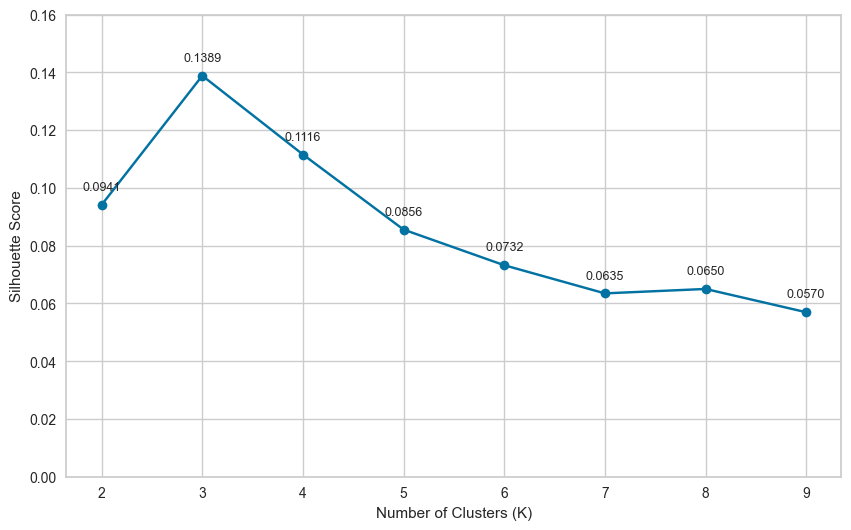
\includegraphics[width=0.7\linewidth]{image/choosing_K.png}
    \caption{Optimal clusters K}
    \label{fig:choosing_K}
\end{figure}

To determine the optimal number of clusters $K$, the K-Modes clustering model is trained with different K values varying from 2 to 9 and select the best model according to the cost function. For each training iteration, the K-Modes algorithm is executed multiple times (15 in our problem) with different initial centroids seeds. The final result is the best initialized centroids in terms of cost function.\citep{devos2015}

After the training is completed, each student is assigned to their predicted cluster, which will be used for the recommendation part.

\subsubsection{Student Recommendation}
Firstly, the information of new student is encoded by one-hot encoding and fed into the model. The output returned is the predicted cluster to which the new student belongs. Depending on this prediction, students within the same cluster are chosen to recommend.

\pagebreak

\section{System Design and Implementation}  
This section describes the detailed process of setting up the system, covering hardware and software configurations, as well as initial testing to ensure all components work seamlessly.
\subsection{Hardware and Software Setup}  
The design and implementation of the system started by setting up the hardware and software environment. Regarding the hardware setup, we have development machines for hosting backend services and the PostgreSQL database, as well as user devices which are mostly Android smartphones or virtual Android devices for accessing features like Schedule view, Campus navigation, and Moodle resources. \\

On the software side, the operating system used for hosting backend services and the database is Window, while Android acted as the primary platform for the mobile application.
For the relational database management system, we choosed PostgreSQL to handle student data, calendar events, location details, and data for StudyBuddy feature.
The backend framework used Spring Boot for managing REST API endpoints, authentication, authorization, as well as data synchronization.
To potentially support the development of the application, we used Android Studio as the main environment for building the application using Java language, as it contains of libraries like Retrofit and MapBox SDK.

\subsection{Application Software} 
The application was divided into several modules, as each of them serve a specific feature.
The Authentication and Authorization Module implemented JWT-based authentication and managed RBAC for ADMIN and USER roles.
The Google Calendar Integration Module was responsible for fetching event data, detecting updates, and notifying students about changes.
The MapBox Integration Module enabled storage of campus's study places coordinates and overall campus map viewing. \\

Regarding Moodle Resource Module, we set up a communication with Moodle APIs to retrieve course materials such as slides, source code, and PDFs.
About StudyBuddy Matching Module, we implemented a machine learning recommendation system to suggest matches based on shared interests, collecting student profile data and offering text-based chat and SIP-based VoIP audio call using the Linphone library.
The Notification System provided real-time alerts for calendar updates and incoming calls.

\subsection{Initial Testing}
To ensure all components were functioning correctly and fully compatible, we conducted initial testing divided into hardware, software, and integration testing. Hardware testing involved verifying the performance and the reliability of development machines, servers, as well as networking environment. 
Regarding software testing, we focused on verifying proper installation, configuration, and performance. The Windows operating system installed on the backend machines was tested for resource allocation, security settings, and reliability.
PostgreSQL was initialized with schemas and sample data, testin with CRUD operations to ensure smooth data handling. 
Spring Boot REST API endpoints were tested individually using Postman to confirm proper functionality, including following the JWT authentication with token. \\ 

Integration testing validated interactions between the various system components. For Google Calendar synchronization, we created dummy events and updated with dummy data to verify proper fetching and real-time notifications.
MapBox integration was tested by checking stored campus location data with real-world coordinates, ensuring the accuracy and functionality for campus navigation on multiple devices, including virtual devices.
Moodle API communication was verified by simulating the process of course material upload and confirmationo of successful retrieval of slides, source code, and PDFs.
Additionally, the StudyBuddy matching feature was tested using both dummy and real profiles to validate the recommendation system, ensuring the high accuracy matches based on profile information.
Chat functionality was tested for text-based messaging and SIP-based VoIP audio calls, with the Linphone library ensuring seamless connection and clear audio quality.
Lastly, the notification system was tested by simulating calendar dummy events updates and incoming calls to confirm notification prompt message.
This testing phase ensured a reliable and fully functional system, ready for deployment.

\pagebreak

\subsection{Application Software}  
The application software comprises several core modules, each designed to handle specific functionalities:  

\begin{itemize}  
    \item \textbf{Authentication and Authorization Module:}  
    \begin{itemize}  
        \item Implements JWT-based authentication.  
        \item Manages RBAC for ADMIN and USER roles.  
    \end{itemize}  

    \item \textbf{Google Calendar Integration Module:}  
    \begin{itemize}  
        \item Fetches event data from Google Calendar.  
        \item Detects event updates and sends notifications to the student via the mobile application.  
    \end{itemize}  

    \item \textbf{MapBox Integration Module:}  
    \begin{itemize}  
        \item Stores campus location coordinates (latitude and longitude).  
        \item Dynamically renders campus maps within the app.  
    \end{itemize}  

    \item \textbf{Moodle Resource Module:}  
    \begin{itemize}  
        \item Communicates with Moodle APIs to retrieve course resources, such as slides, source code, and PDFs.  
    \end{itemize}  

    \item \textbf{StudyBuddy Matching Module:}  
    \begin{itemize}  
        \item Collects student profile data (e.g., interests, personality).  
        \item Uses a machine learning recommendation system to suggest matches based on shared interests.  
        \item Features include:  
        \begin{itemize}  
            \item Chat functionality for text-based communication.  
            \item Audio calling capabilities powered by the Linphone library, which provides SIP-based VoIP functionality.  
        \end{itemize}  
    \end{itemize}  

    \item \textbf{Notification System:}  
    \begin{itemize}  
        \item Delivers real-time notifications for calendar updates and incoming calls.  
    \end{itemize}  
\end{itemize}

\pagebreak

\subsection{Initial Testing}  
Extensive testing ensured all components functioned correctly and integrated seamlessly:  

\begin{itemize}  
    \item \textbf{Hardware Testing:}  
    \begin{itemize}  
        \item Verified the setup and operation of development machines, servers, and networking equipment using Tailscale VPN for secure communication.  
    \end{itemize}  

    \item \textbf{Software Testing:}  
    \begin{itemize}  
        \item Tested the configuration and performance of the operating system, PostgreSQL database, and Spring Boot services.  
    \end{itemize}  

    \item \textbf{Integration Testing:}  
    \begin{itemize}  
        \item Validated the interaction between backend APIs and mobile app features, ensuring functionality for:  
        \begin{itemize}  
            \item Google Calendar synchronization.  
            \item MapBox map rendering.  
            \item Moodle resource retrieval.  
            \item StudyBuddy matching and chat capabilities.  
            \item Linphone-based audio calling.  
        \end{itemize}  
    \end{itemize}  
\end{itemize}

\pagebreak

\section{Results and Discussion}
This section focus on the results and discuss the outcome of the USTH Connect project, focusing on key aspects such as model performance, application development progress, and challenges we encounter during the development.
\subsection{Results}

\subsubsection{Mobile App Results}
In this part we will show the result of the application developement, mainly about what we have developed so far and some specific results of the application. \\

\textbf{Application Features Progress} \\

The USTH Connect mobile application has made significant progress in its development, results in successful implementation of several features.
Apart from the configuration of login and registration system using JWT authentication and RBAC, we manage to develop a functions for synchronizing calendar events with the school's Google Calendar.
In our application, we have displayed the schedule according to the student's major and study year to save student effort finding the correct schedule. 
Moreover, students can view all the lectures events for a specific subject. Also, the system periodically fetchs events and detects event changes to notify the students about their schedule.
We have configured a map feature using MapBox SDK to display campus maps with location markers for each buildings and facilities which supports student efficiently navigate within the university.
Regarding lecture resources, we have successfully linked the application to Moodle, allowing students to retrieve and view course materials directly from the app.
For the main feature StudyBuddy, we have developed a recommendation system using machine learning model. By retrieving student's data, we can successfully return and display a list of compatible partners for students to enrich their social life.
The app provides a chat platform and audio call using Linphone VoIP library for real-time communication between matched students. Especially, the audio call has been improved with real-time connection and notifications. 
However, the chat platform yet does not have a notification for incoming messages and more appealing UI for better application experience.
Also, we have not figure out an efficient way to store the image to support Study Buddy feature in displaying images for each users. \\

\textbf{Mobile-Specific Results} \\

We tested across a variety of devices (emulator and Android) and the performance was consistent, with the two main factors: App Launch Time and Network Usage. The average app launch time was 2 seconds on Android devices and 4 seconds on Emulator devices. The app also optimized data usage by caching schedule events, map location and course materials, which partly reduce a dependency on continuous internet access for those features. 
By combining many features of other applications into one, USTH Connect offer students an efficient tool. This eliminates the need for multiple applications, saving students time and enhancing their overall experience.

\subsubsection{Machine Learning Results}
In this part we will show the result of the clustering algorithm, using the evaluation of
metrics that we mentioned in the previous section. \\

\textbf{Model Performance} \\

\begin{table}[H]
\centering
\resizebox{0.7\textwidth}{!}{%
\begin{tabular}{|c|c|c|}
\hline
\textbf{Model} & \textbf{Silhouette Score} & \textbf{Davies-Bouldin Score} \\ \hline
K-Modes & 0.1389 & 3.4489 \\ \hline
\end{tabular}%
}
\caption{Model Performance}
\label{Model_Performance}
\end{table}

Table \ref{Model_Performance} presents the values of the Silhouette and Davies-Bouldin score. The silhouette score indicates how close the data point is to its cluster compared to the others, while the Davies-Bouldin score shows how high the overall quality of the clustering model. With a Silhouette score of 0.1389 and a Davies-Bouldin score of 3.4489, the centroids of each cluster are relatively close to each other, and the boundaries between clusters may not be ideal.\\

The same pre-processing method and K-Modes model is also applied to the Zoo dataset (with true label) and gives the result: 0.5362 of Silhouette Score and 1.21 of Davies-Bouldin Score. The Kuhn-Munkres\citep{zhu2011efficient} algorithm is used to match predicted clusters with the true types of animals to maximize accuracy. This performance is notably better than the results obtained in our dataset. The possible reason for this may be the higher dimensionality of the input data in our dataset, which can increase noise and complexity for clustering.\\ 

\textbf{Similar System} \\

The same pre-preocessing method and K-Modes model is applied to the Zoo dataset (with true label) and gives the result: 0.5362 of Silhouette Score and 1.21 of Davies-Bouldin Score. The Kuhn-Munkres\citep{zhu2011efficient} algorithm is used to match the predicted clusters with the true types of animals to maximize accuracy.

\subsection{Discussion}
\subsubsection{Intepretation of Results}
The development of USTH Connect has show significant progress in creating a comprehensive mobile application designed to improve university life.
The app efficiently combines various features, including Google Calendar synchronization, campus naviation, access to Moodle resources, and the StudyBuddy recommendation system.

Although the clustering algorithm provides valuable insights into study partner compatibility, evaluation metrics indicates that the need of improvement in cluster separation and cohesion.
The low Silhouette score and high Davies-Bouldin score show the need for better feature selection or model tuning to enhance clustering performance. \\

Regarding the mobile application, fetching and caching data like schedules and course materials has dramatically enhanced usability, enabling partial offline access.
However, the lack of chat message notifications and a more optimized image storage system reduce the overall user experience.

\pagebreak

\subsubsection{Comparison to Similar System}
Unlike traditional university assistance apps that mostly focus on course and student management or navigation, USTH Connect combines multiple features into a single application, implementing academic tools with a social networking developed by machine learning.
In contrast to other platforms which may recommend compatible groups or clubs, USTH Connect's StudyBuddy feature offers a more personalized study partner recommendation system.
In terms of user experience, many similar systems lack seamless communication methods, such as real-time audio calling with real-time notification, which is one of the features that USTH Connect offers.
However, the need of improvements in UI design and notification system to surpass other platforms.

\subsubsection{Challenges and Limitations}
Despite the progress made, the project faced serveral challenges and limitations. First, the current system for storing and retrieving student images in the StudyBuddy feature is inefficient, resulting in a poor user experience and diminishing the visual appeal of the interface. Additionally, the performance of the clustering algorithm indicates the need for further research in feature selection, parameter tuning, or exploring alternative algorithms to optimize its effectiveness. While notifications for calendar events and VoIP calls are functioning as expected, the system lacks of notifications for incoming chat messages and matched partners in the StudyBuddy feature, which needs to be addressed. Furthermore, certain sections of the app, such as the chat interface and the StudyBuddy partner profile view, require improved visual design and user-friendly features to enhance the overall user experience. About the cross-device testing problem, although the application has been tested on emulators and Android devices, broader cross-device testing is necessary to ensure compatibility across different screen sizes and operating system versions. Another critical aspect is the Moodle integration, where the app currently relies on a custom-built Moodle system rather than integrating with the official Moodle platform provided by the school. This limitation prevents synchronization with official course materials, restricting students' seamless access to academic resources and course content. Full integration with the official Moodle platform is essential to enhance the app’s functionality and provide students with comprehensive support for their academic needs.
% \begin{itemize}
%     \item \textbf{StudyBuddy Image Storage: } The current system for storing and retrieving student images is inefficient, leading to poor user experience and negatively affecting the expected appealing interface of the feature.
%     \item \textbf{Clustering Model Optimization: } The current performance of the clustering algorithm points out the need for further research in feature selection, parameter tuning, or the consideration of alternative algorithms.
%     \item \textbf{Notification System: } While notifications for calendar events and VoIP calls are working as expected, the chat feature lacks the notifications for incoming messages, and the notification for the matched partner in the StudyBuddy feature. 
%     \item \textbf{UI/UX Design: } Some sections of the app, like chat interfaces and StudyBuddy partners profile view, need improved visual and user-friendly design to enhance the user experience.
%     \item \textbf{Cross-Device Testing: } Although testing was done on emulators and Android devices, more testing across different screen size and operating system version is necessary to comprehensively optimize the application.
%     \item \textbf{Moodle Integration: } Currently, the app uses a custom built Moodle system rather than integrating with the official Moodle platform provided by the school. This limitations prevent the synchronization with official course materials available on the university's Moodle. Full integration with the actual Moodle platform is necessary to provided students with seamless access to their course materials and academic resources.
% \end{itemize}

\pagebreak

\section{Conclusion {\&} Future Work}
\subsection{Conclusion}
The USTH Connect mobile application has achieved significant progress in implementing essential university functions into a single platform. Features like calendar synchronization, campus naviation, Moodle integration, and the StudyBuddy recommendation system help simplify and improve student life.
Along with obtained successes, some challenges are still there, especially in improving chat features, refining StudyBuddy features, and optimizing the clustering algorithm.
The StudyBuddy feature's machine learning model indicates the need of improvement, especially the clustering algorithm's performance. The Silhouette and Davies-Bouldin scores suggest that the current model's cluster separation is not efficient as expected, which requires the further improving of the feature. \\

On the other hand, the app's ability to fetch, manage and cache data for offline access, combined with real-time communication features such as audio calling and notifications, which improves the overall user experience. \\

In summary, USTH connect has shown potential in becoming a vital tools for students at the University of Science and Technology of Hanoi, enhancing their academic and social experiences. 
Despite some challenges, its development is positive, and with future improvement, it can become a fully integrated, user-friendly application.

\subsection{Future Work}
To contribute to the current achievements of USTH Connect and address its existing limitations, future development will focus on several key areas. 
Enhancing the StudyBuddy is our first priority, as it is our key feature of the application, involving the improvement of the machine learning model used for recommending study partners.
We will find an alternative clustering algorithms, refining the feature selection process, and optimizing the image storage system for user profiles to improve the user experience to the full extent. \\

Improving the application's user interface is another significant section that we need to focus on. 
Sections like the chat interface, the StudyBuddy profile views, and other areas will be refined to improve the overall visual and make user more engaged into our application.
To declare the problems about our user interface, user feedback play a vital role in creating these enhancement suggestion to verify a design that match the student expectations and preferences.
Additionally, optimizing the notification system will be a key improvement as it associates with many key functionalities like schedule retrieval and StudyBuddy communication features.
We will focus to enable a notification for chat features, as well as notify users about new StudyBuddy matches and importance calendar events such as Exam day or Meetings. \\

Regarding the clusteing algorithm, the current one for StudyBuddy feature will need further optimization through testing alternative methods, fine-tuning parameters, and combining additional relevant features to improve the accuracy of the recommendation. Moreover, the model performance could be improved by reducing the dimensionality of the input data and integrating deep learning for features extraction. With this integration, the model can reduce noise features while still retain the characteristics of user. After the application is running, user behaviors such as the number of likes, time spent on recommending part, and the number of connected friends will be collected for further analysis and better user experience understanding. 
Similarly, the platform compatibility and cross-device testing will be improved to ensure the application performs consistently across various screen sizes and operating systems.
This work will help deliver a more unique and unified experience for all users. \\

Moreover, full integration with the university's Moodle system is necessary to provide students with up-to-date course materials and academic resources. 
Finally, future versions of the application will introduce more features based on our user feedback, enabling USTH Connect to address their needs and contribute more to the improvement of USTH student's university life. \\

By addressing these key areas, USTH Connect can evolve to meet the growing needs of students, providing even greater benefits to both users and the university community. The continuous development of the app will ensures the valuable and vital tools for students.
Through future improvements, USTH Connect has the potential to become a necessary platform that supports both academic and social activities, as well as encourage a more connected and engaged academic environment.

% To contribute to the successes of the current USTH Connect and address its limitations, future work will focus on several key areas:
% \begin{itemize}
%     \item \textbf{Enhancing the StudyBuddy feature: } The current machine learning model for recommending study partners can be improved by exploring different clustering algorithms or refining the feature selection process. Additionally, the image storage system for user profiles needs opimization to enhance visual interface and adapt with the larger user base.
%     \item \textbf{Improving UI/UX: } Upgrading the UI/UX, especially in sections like the chat interface, StudyBuddy profile views, and other sections, will significantly enhances the user experience. Deploying the app and gathering user feedback on design will be essential to make the app more intuitive and appealing.
%     \item \textbf{Optimizing Notifications Systems: } The notification system for the chat features needs improvement to ensure students have a better experience when using the chat features. Beside, notifications for new StudyBuddy matches and important calendar events should also be optimized to improve user interaction.
%     \item \textbf{Refining the Clustering Algorithm: } The existing clustering model can be optimized by fine-tuning its parameters, testing alternative clustering techniques, and introducing additional features to improve the prediction accuracy.
%     \item \textbf{Platform Compatibility and Cross-Device Testing: } To ensure broad compatibility, the app needs to be thoroughly tested across different screen sizes and operating systems beyond Android devices and emulators. This will help deliver a consistent user experience across all platforms.
%     \item \textbf{Integration with Moodle: } Having full integration with the university's Moodle system will be vital for providing students with up-to-date course materials and academic resources.
%     \item \textbf{Expanding Additional Features} After deploying the app, using user feedback and needs, future versions of USTH Connect could introduce additional features to further enhance its value.
% \end{itemize}
% By addressing these key areas, USTH Connect can evolve to meet the growing needs of students, providing even greater benefits to both users and the university community. The continuous development of the app will ensures the valuable and vital tools for students.
% Through future improvements, USTH Connect has the potential to become a necessary platform that supports both academic and social activities, as well as encourage a more connected and engaged academic environment.

\pagebreak
\renewcommand{\bibname}{REFERENCES} 
\addcontentsline{toc}{section}{References}
\begingroup
\bibliographystyle{IEEEtran} 
\bibliography{bibliography} 
\endgroup

\pagebreak

\appendix
\section*{Appendices}
\addcontentsline{toc}{section}{Appendices} 

\begin{figure}[H]
        \centering
        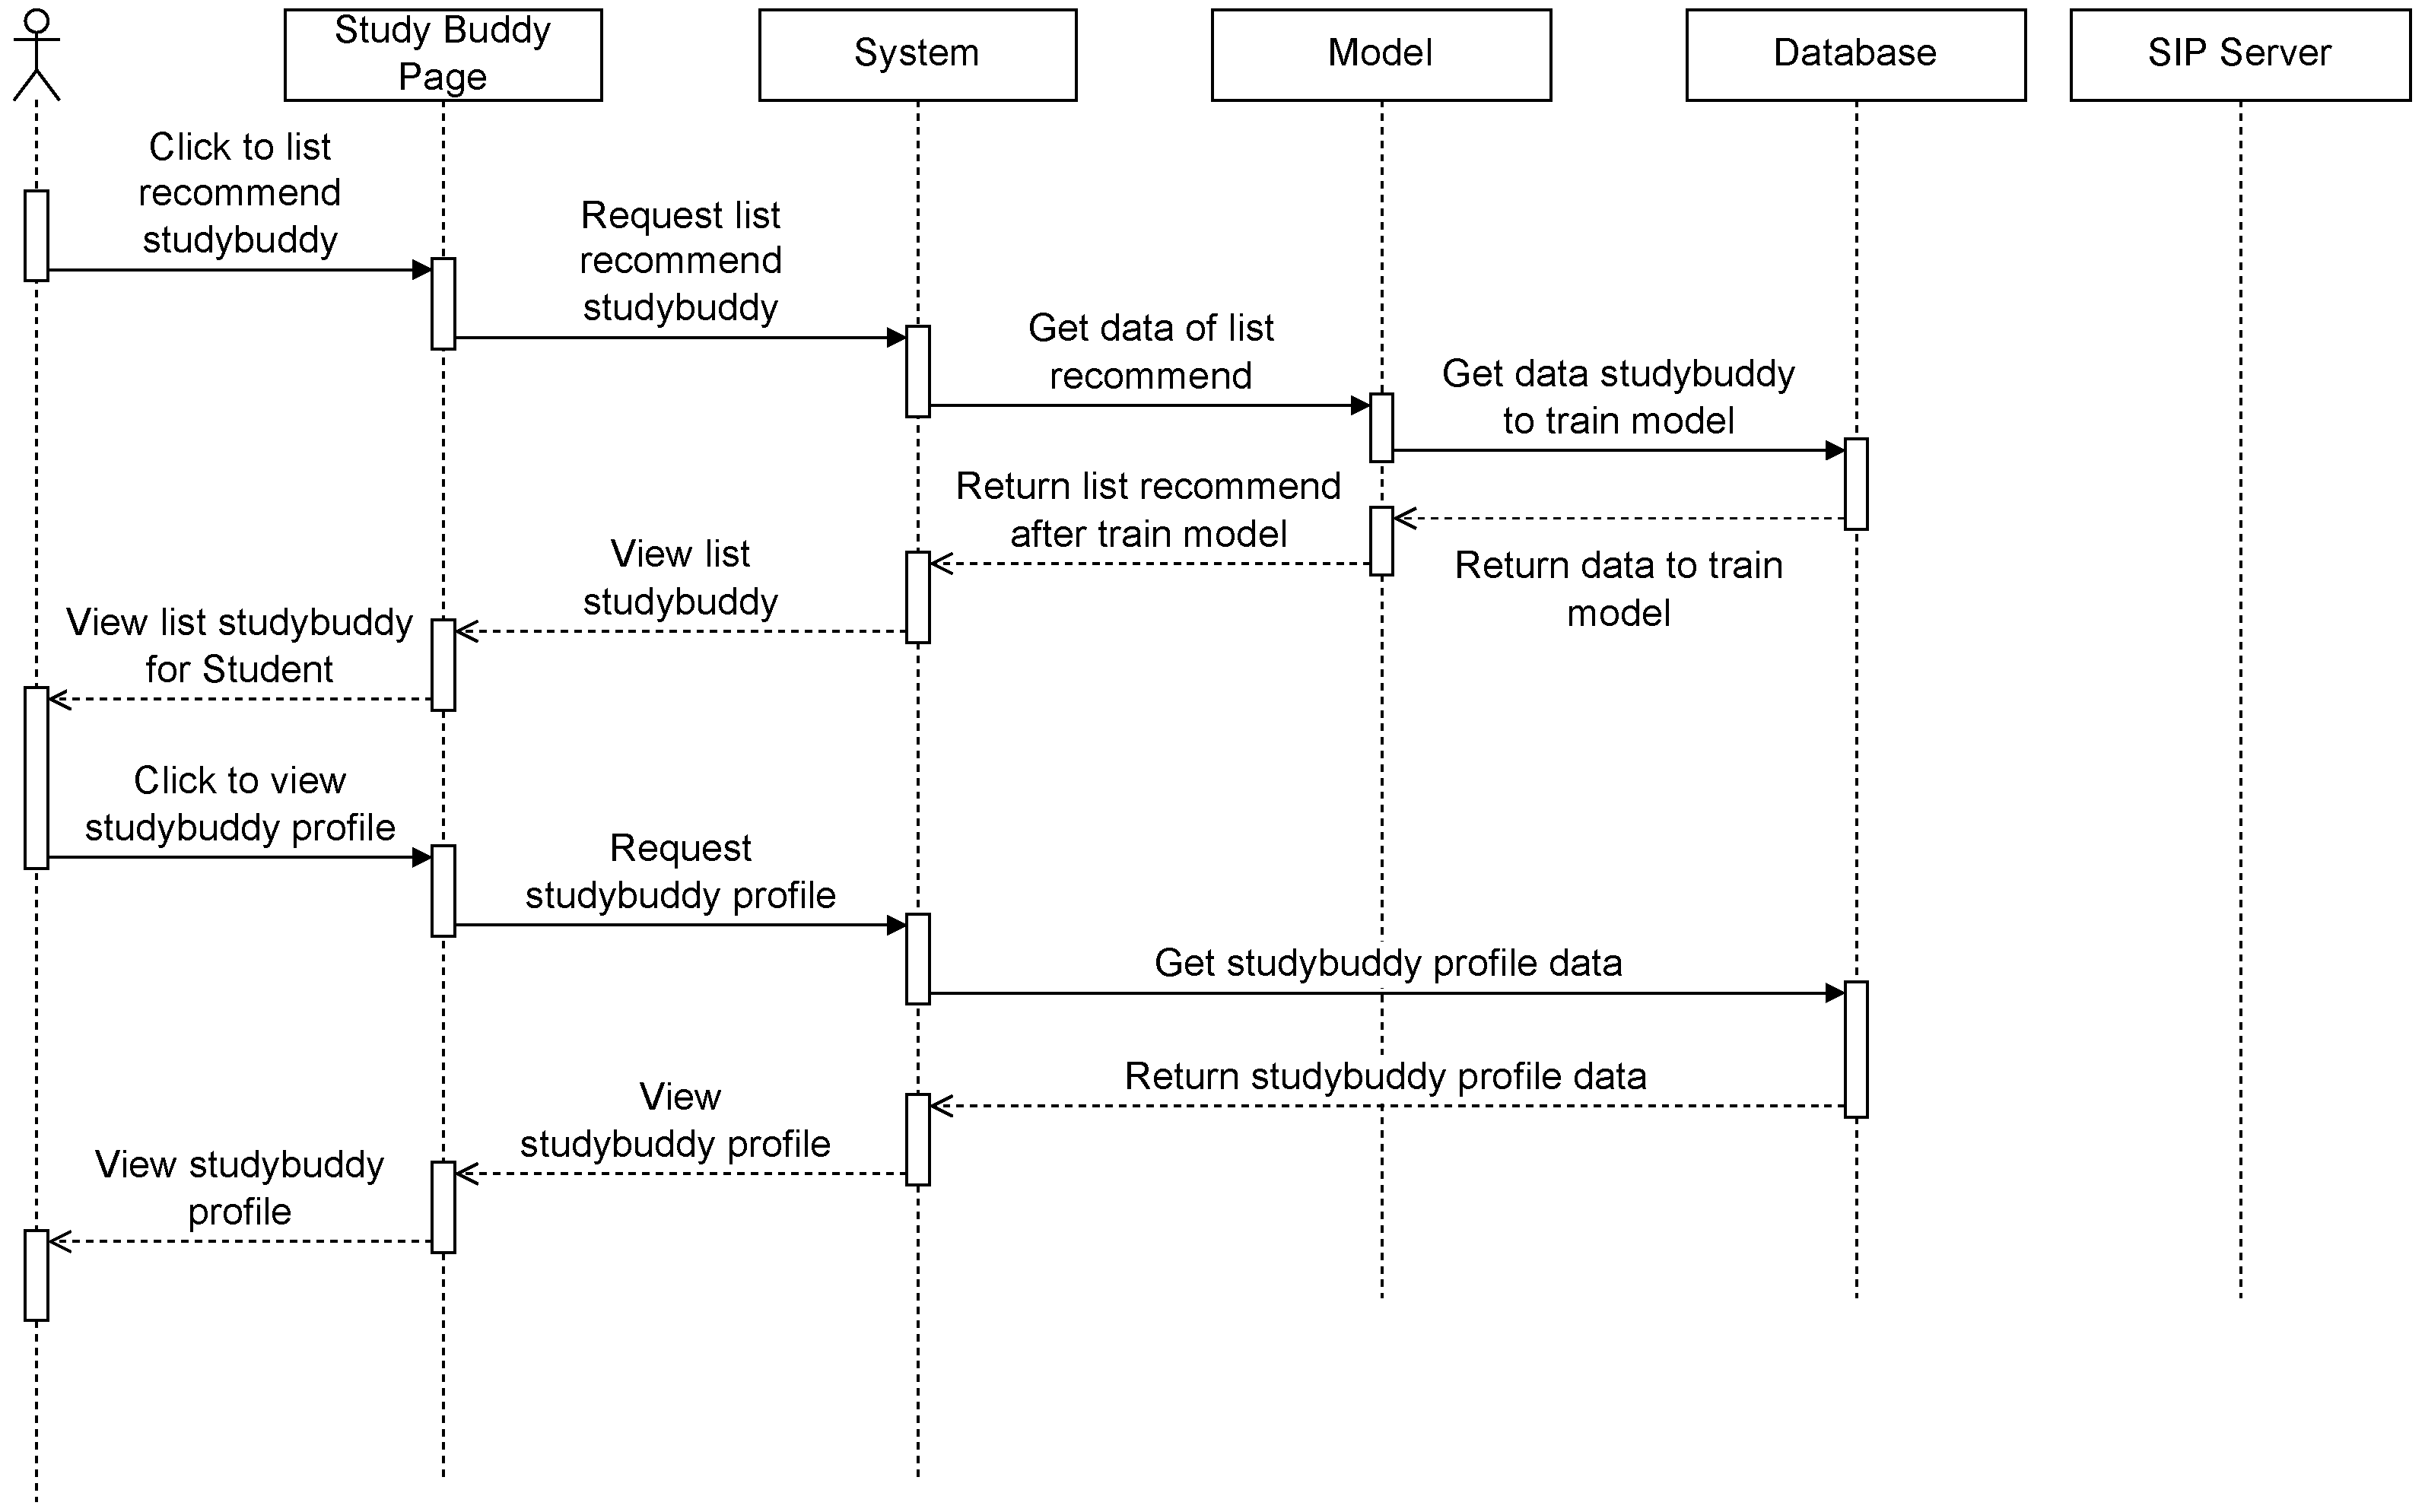
\includegraphics[width=1\textwidth]{image/StudyBuddySequenceDiagram-SB.pdf} 
        \caption{Study Buddy recommend list sequence diagram}
        \label{fig:studyBuddy_recommendlist_sequence}
    \end{figure}

    \begin{figure}[H]
        \centering
        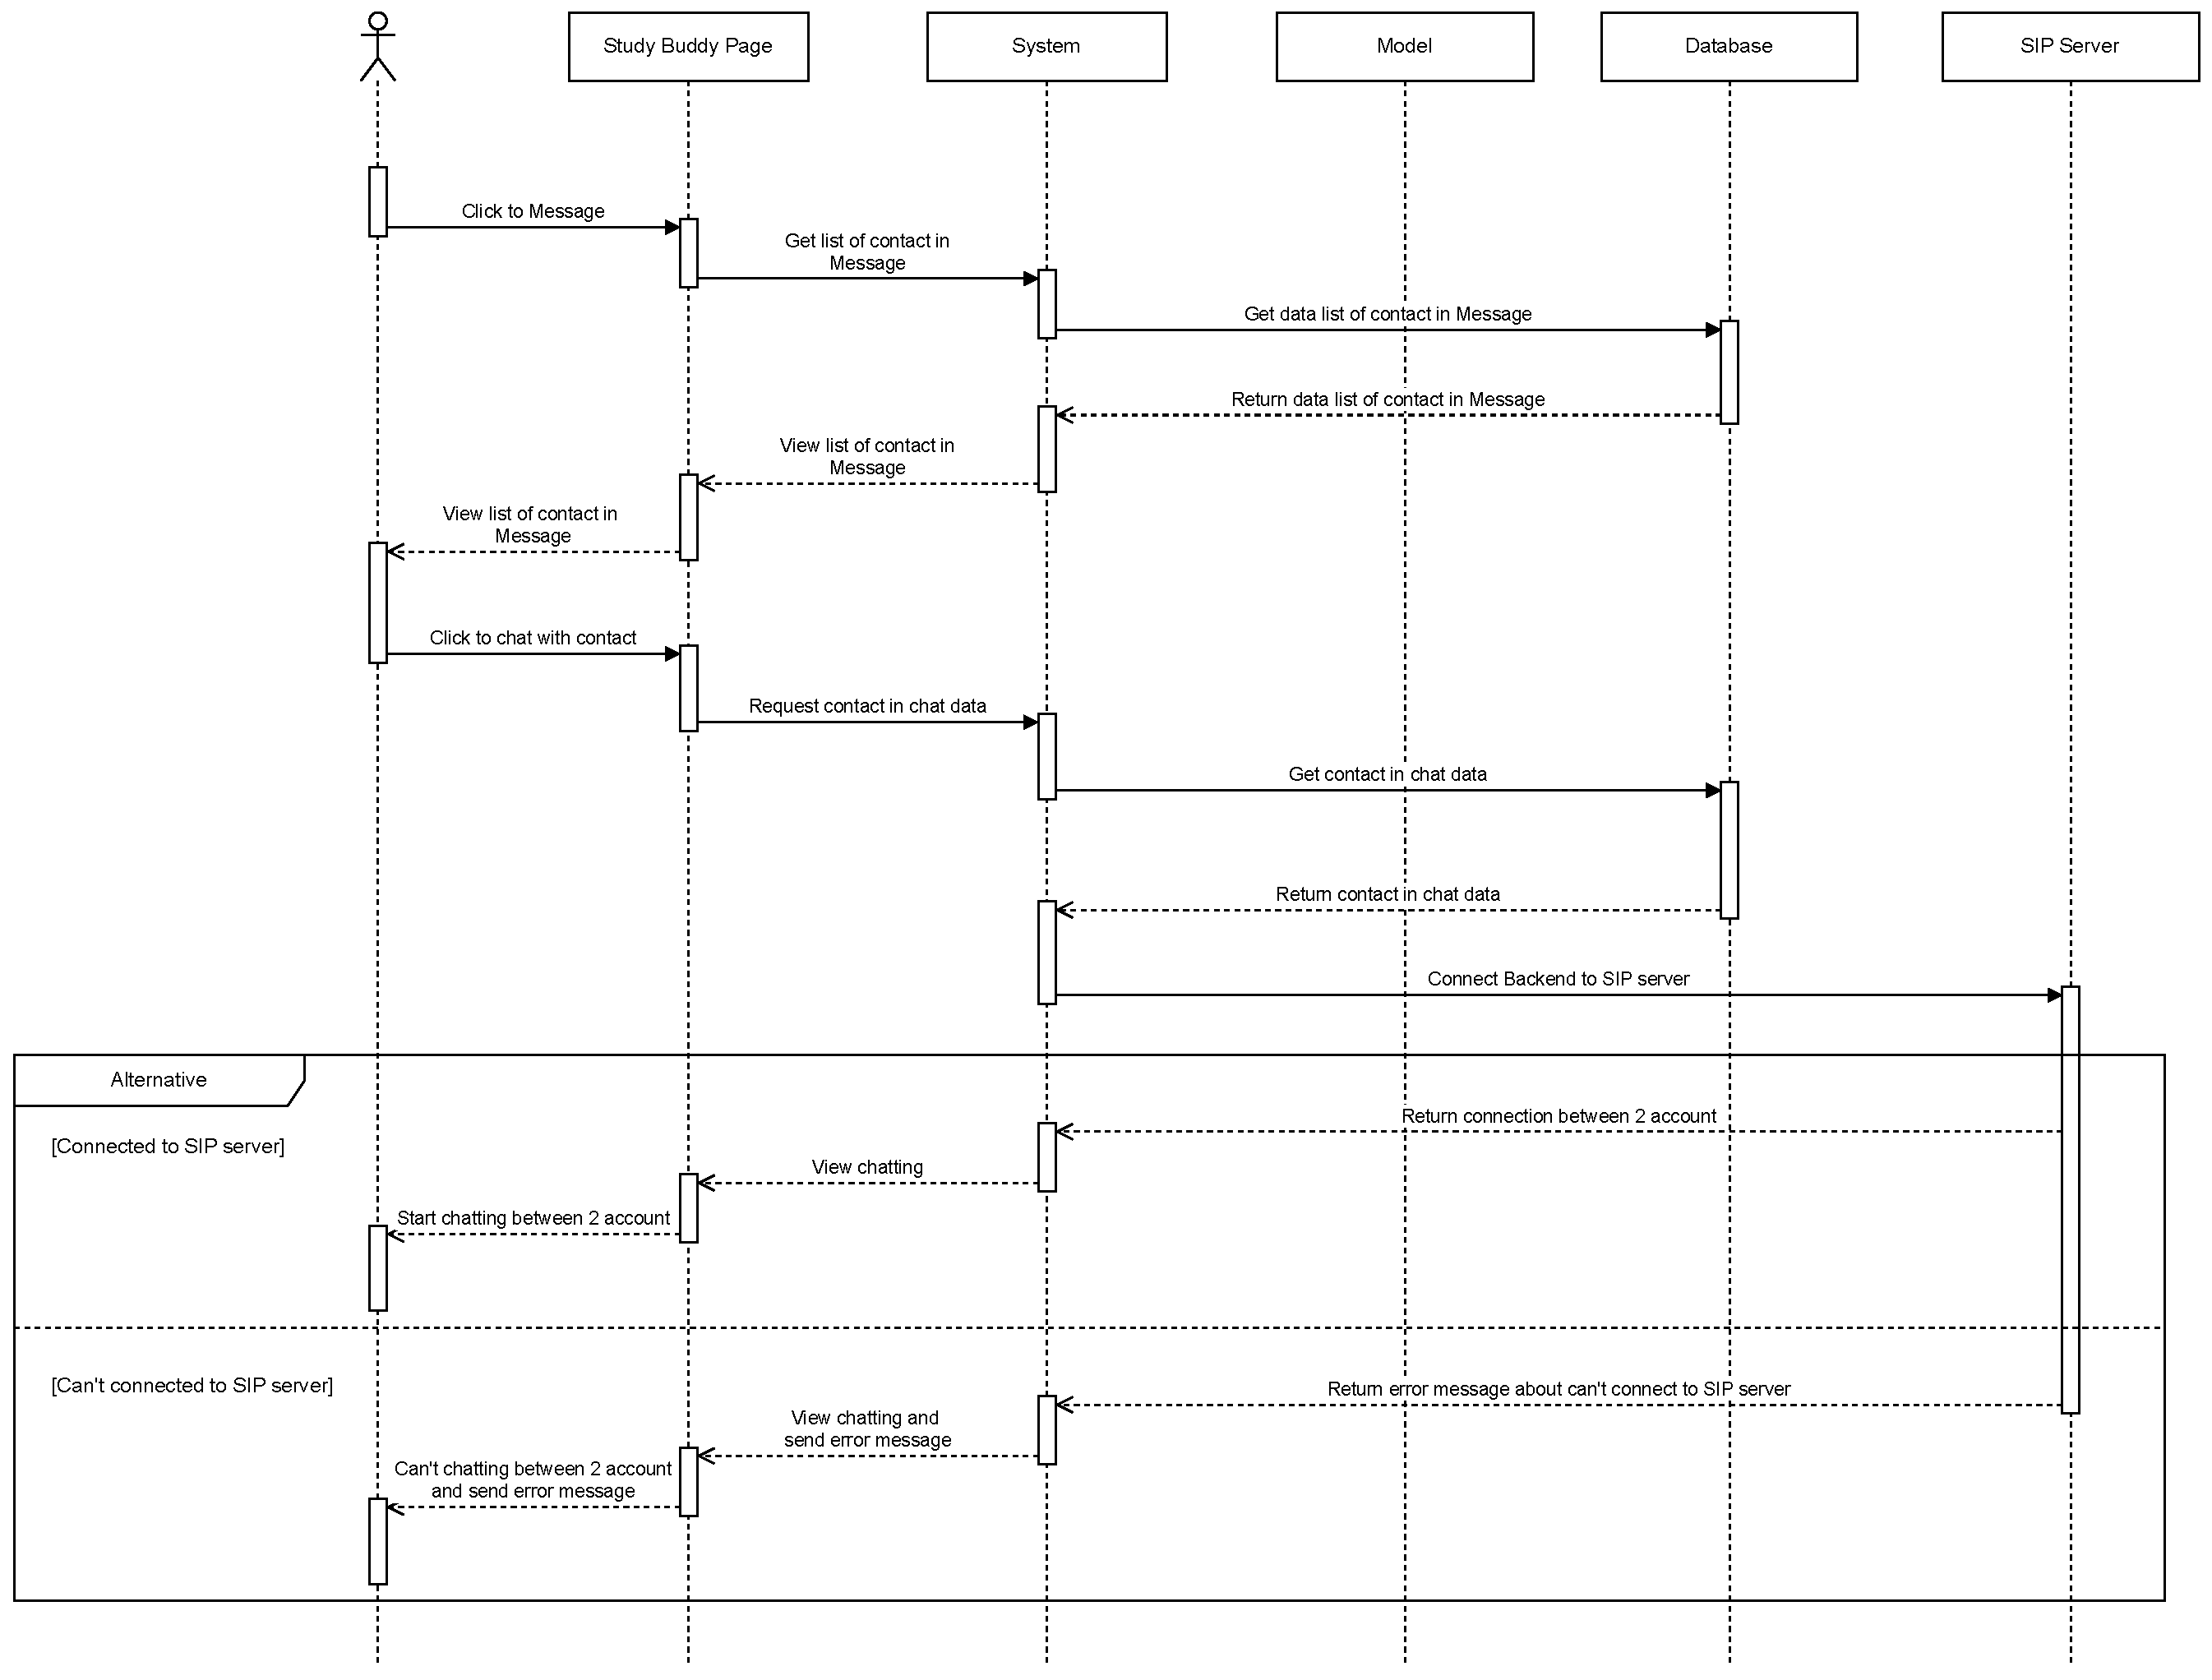
\includegraphics[width=1\textwidth, height=0.5\textheight]{image/StudyBuddySequenceDiagram-Message.pdf} 
        \caption{Study Buddy chat message sequence diagram}
        \label{fig:studyBuddy_chatmessage_sequence}
    \end{figure}

    \begin{figure}[H]
        \centering
        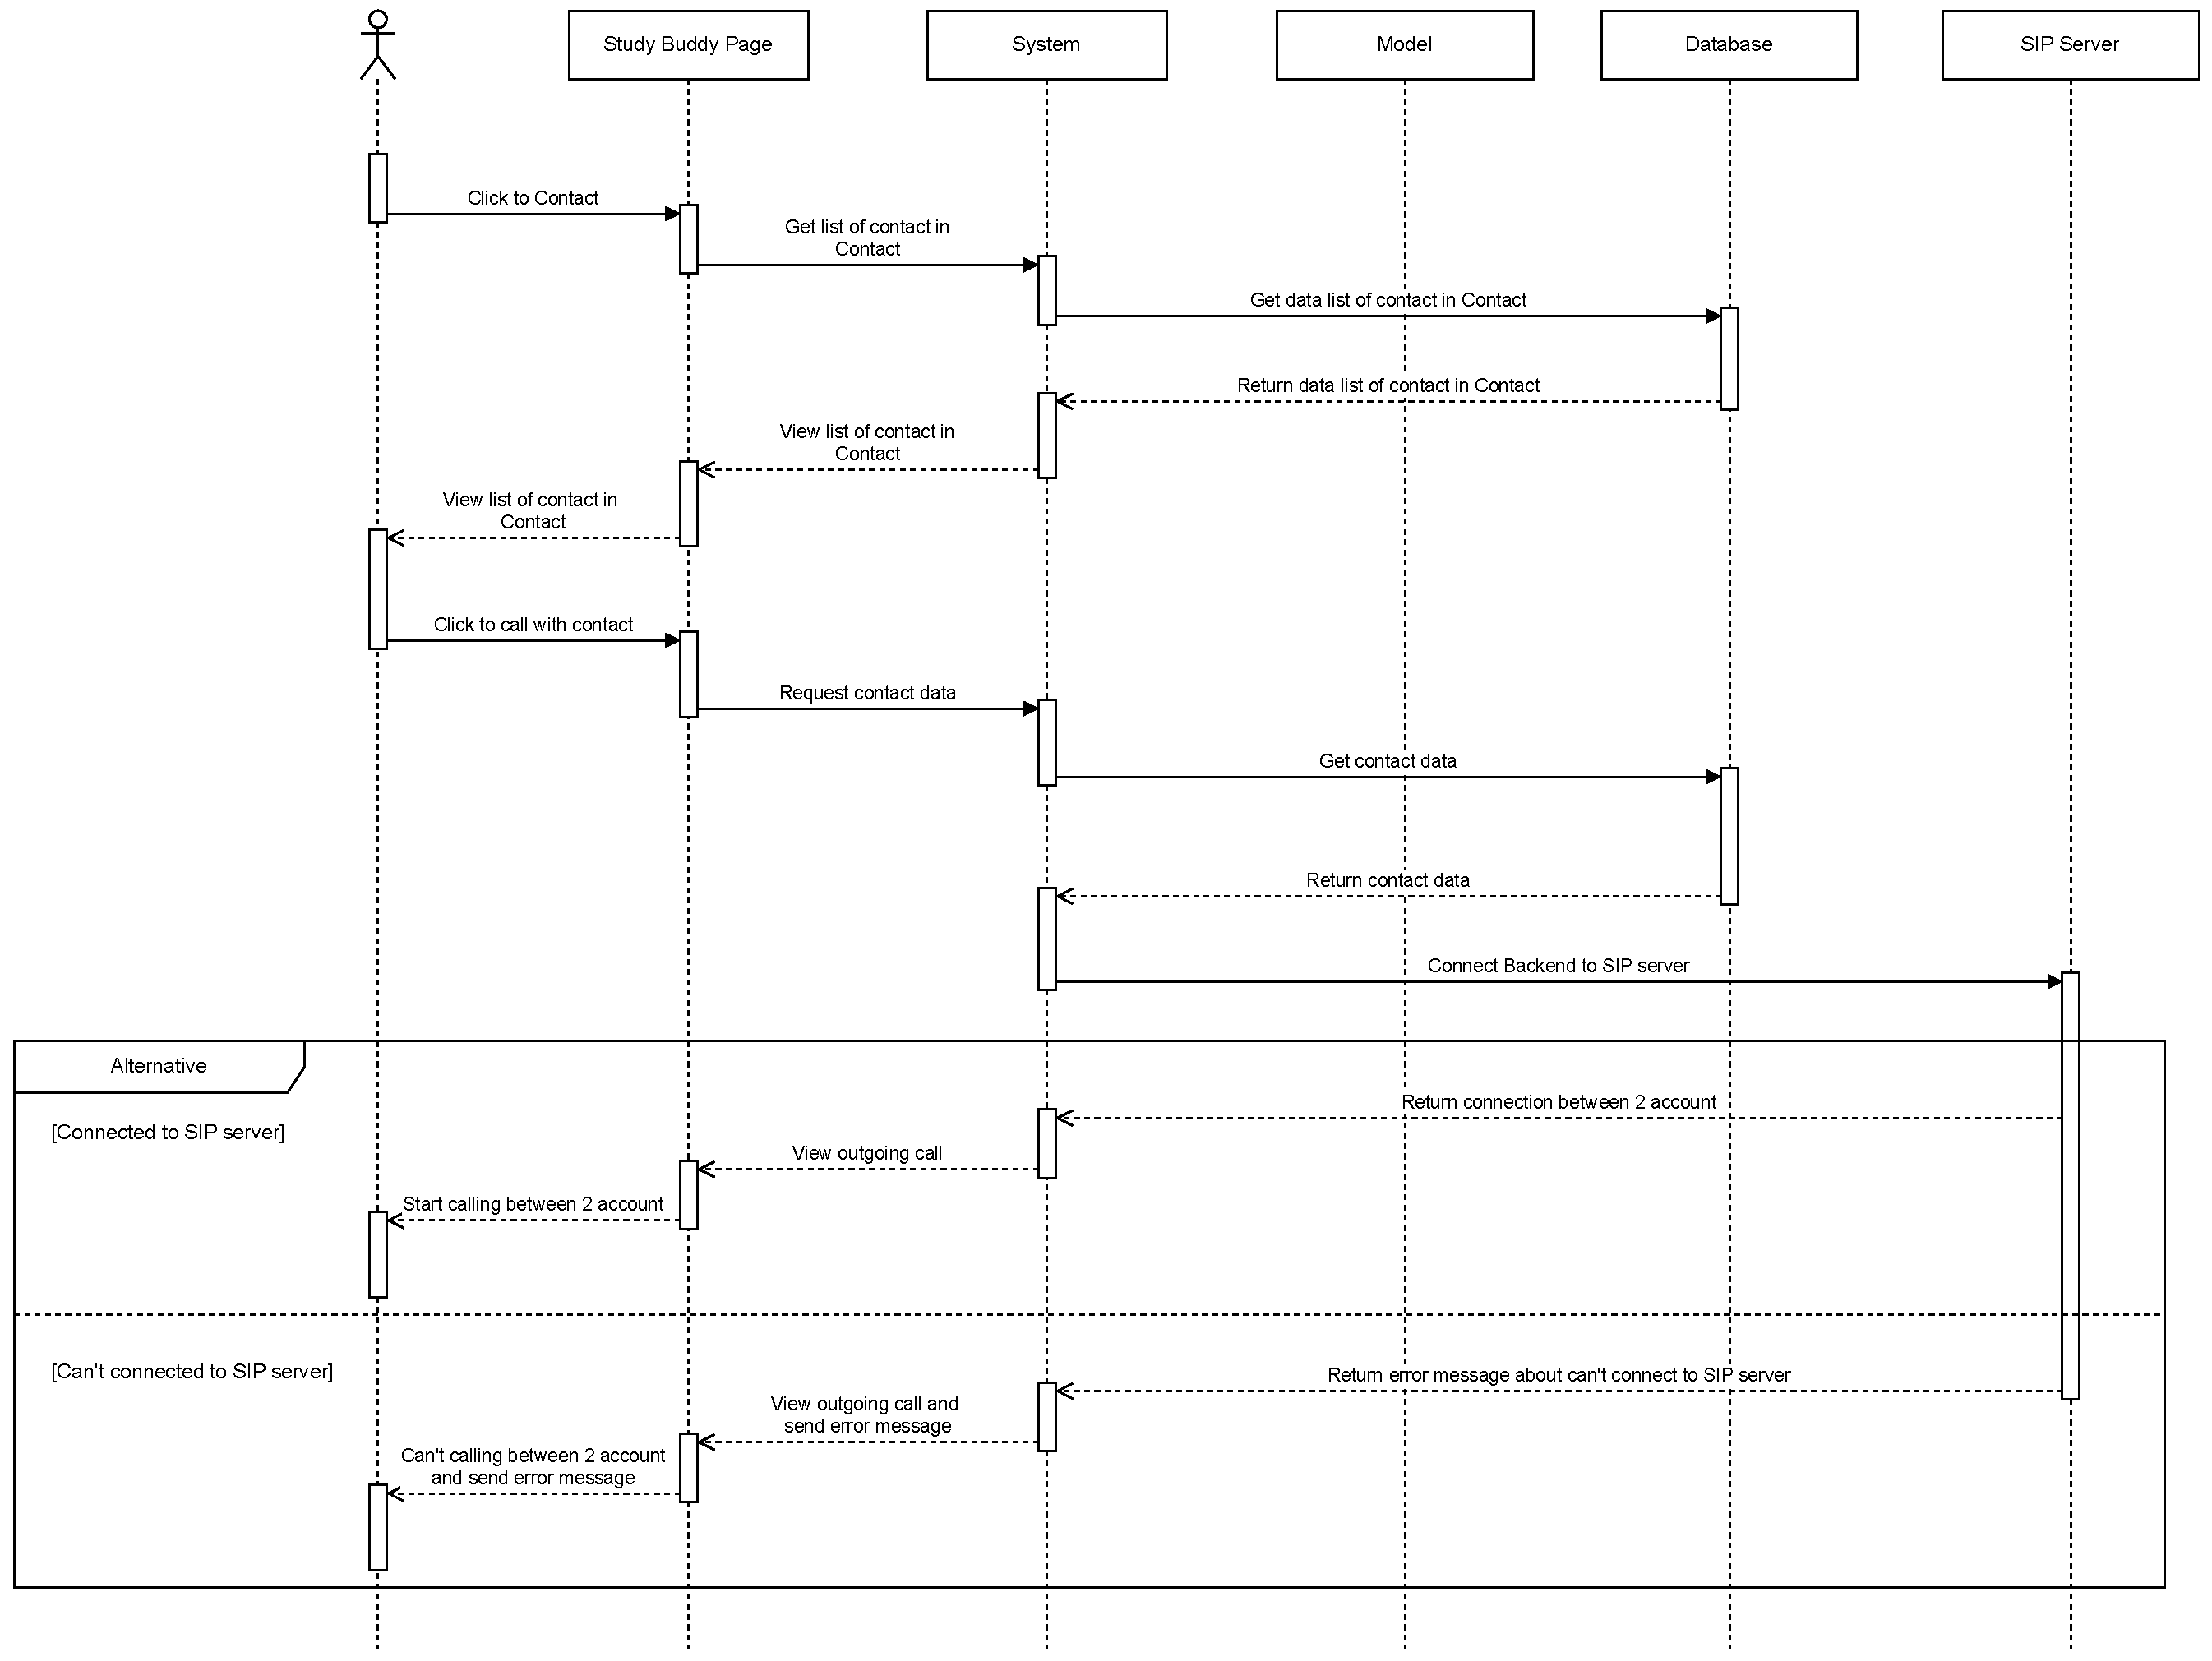
\includegraphics[width=1\textwidth, height=0.5\textheight]{image/StudyBuddySequenceDiagram-Contact.pdf} 
        \caption{Study Buddy audio call sequence diagram}
        \label{fig:studyBuddy_audiocall_sequence}
    \end{figure}

    \begin{figure}[H]
        \centering
        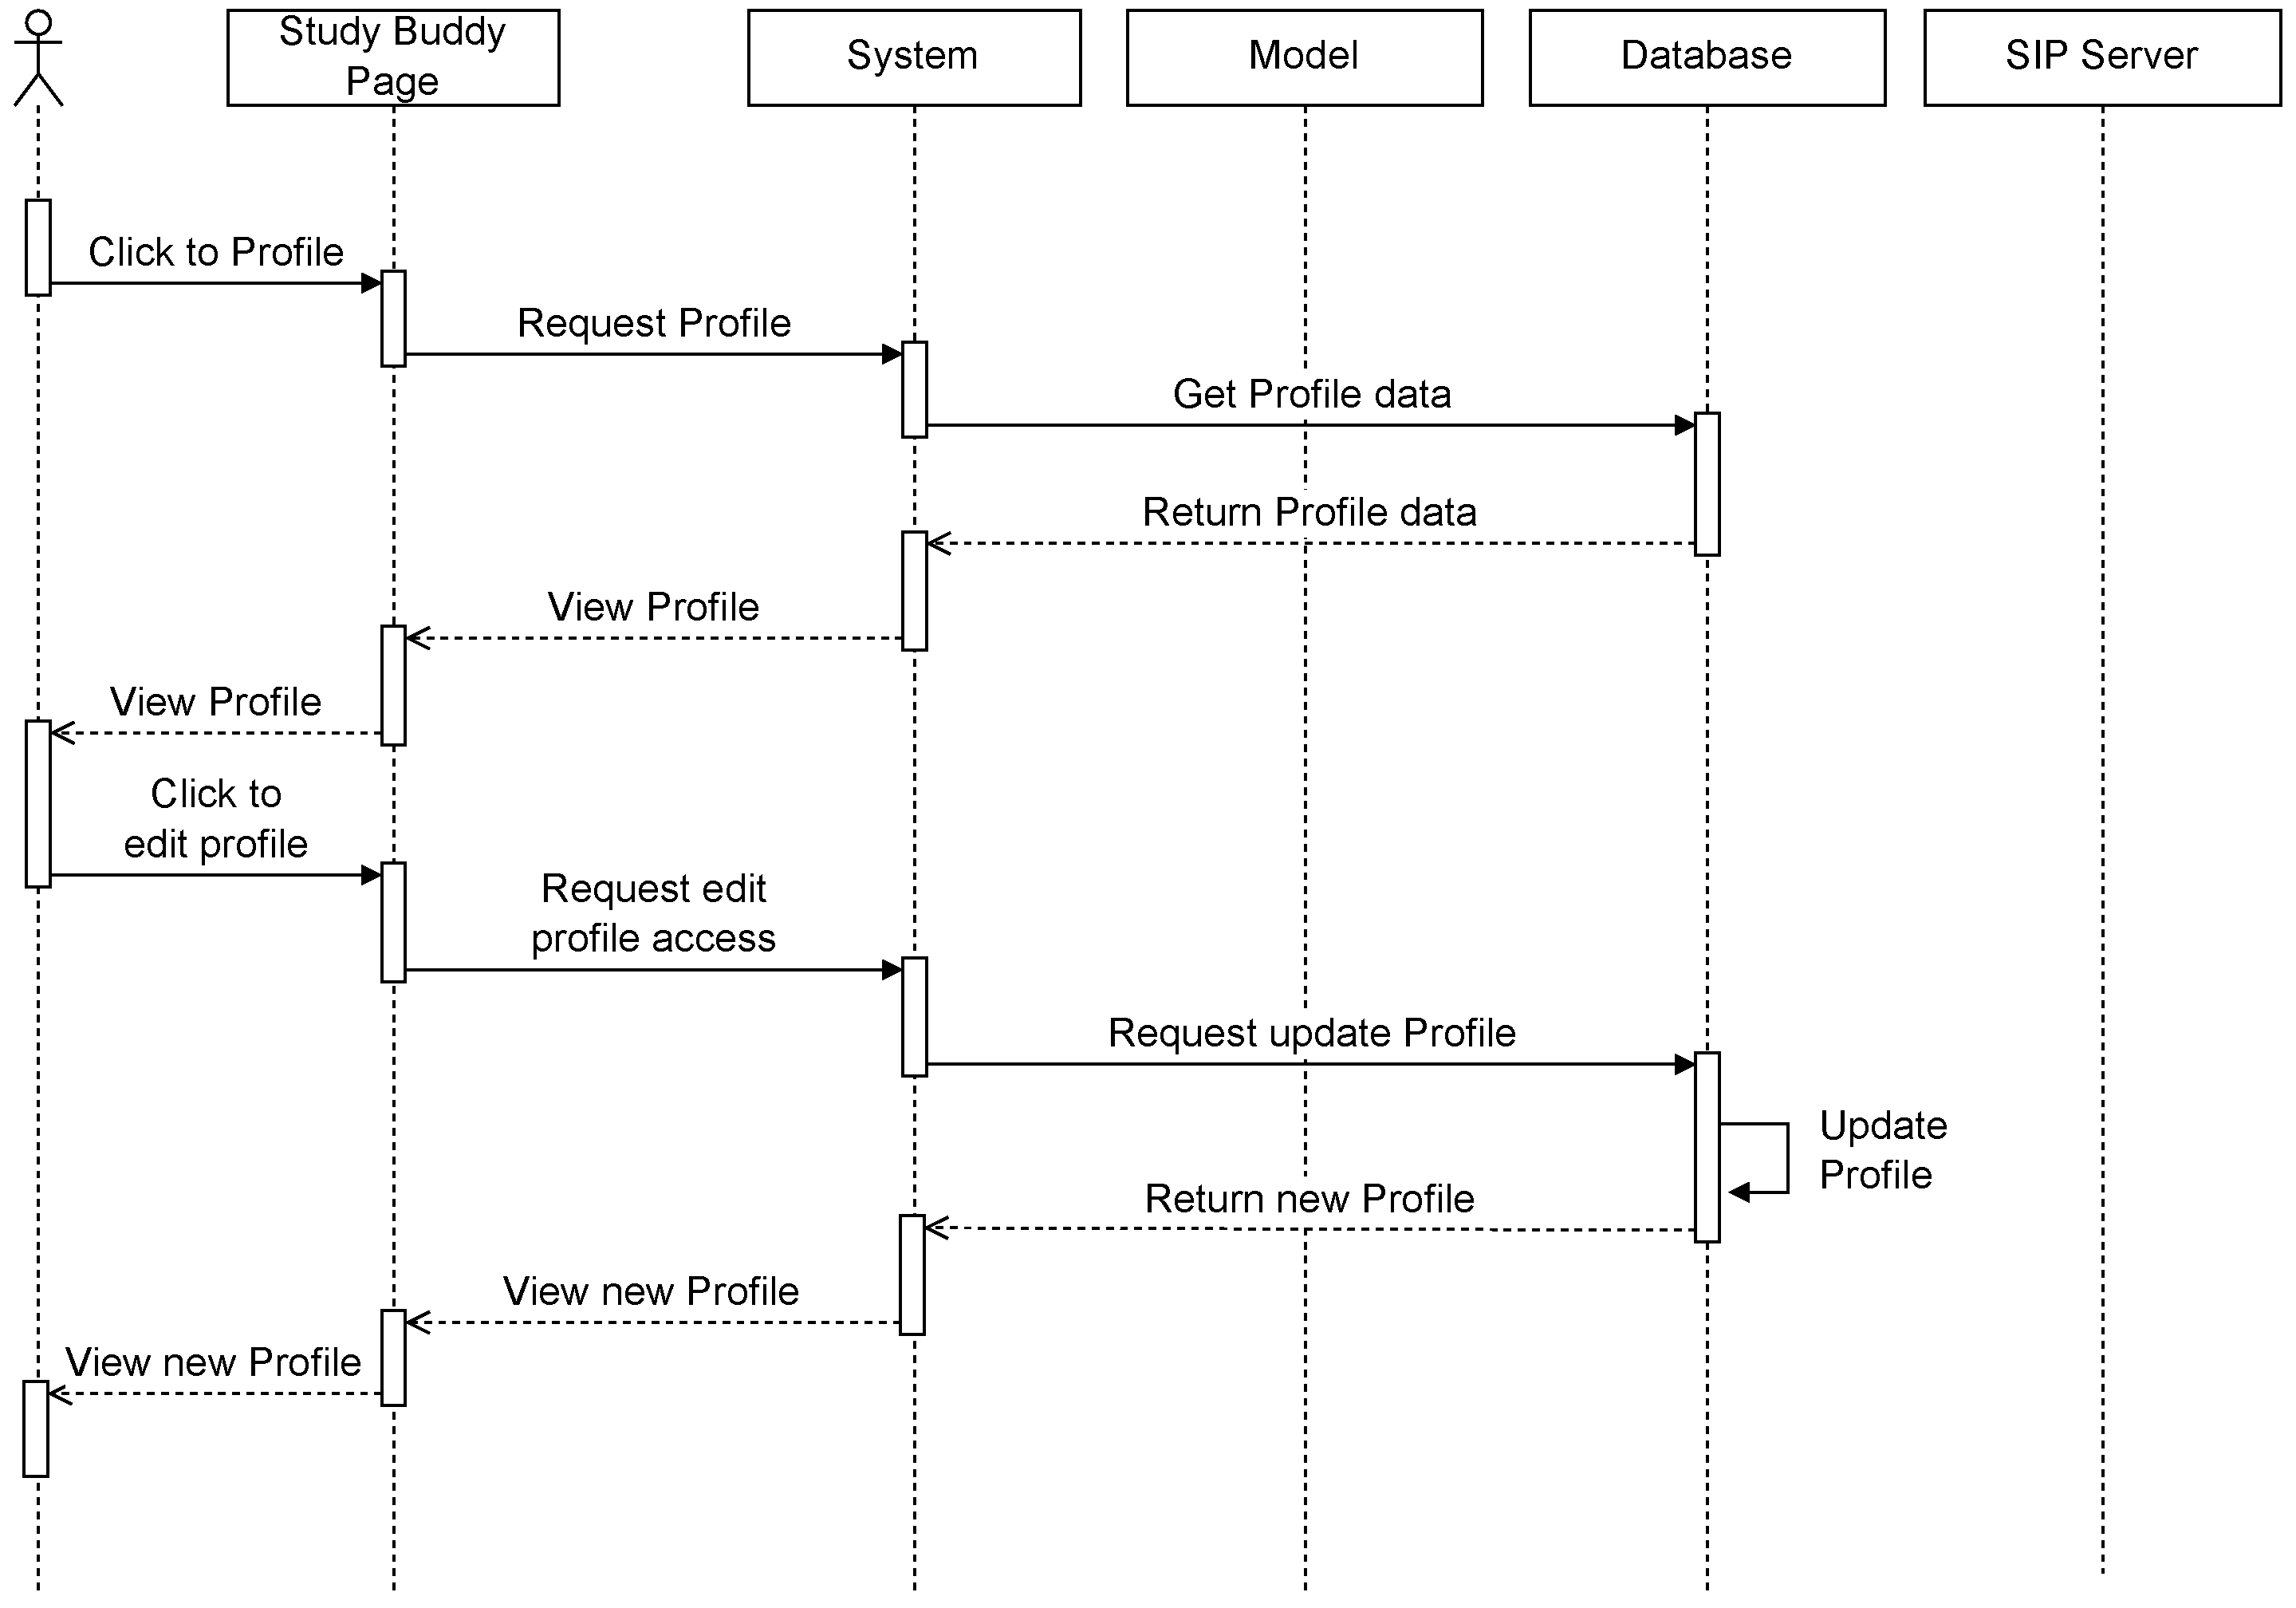
\includegraphics[width=1\textwidth]{image/StudyBuddySequenceDiagram-Profile.pdf} 
        \caption{Study Buddy profile sequence diagram}
        \label{fig:studyBuddy_profile_sequence}
    \end{figure}



    \textbf{Table: Organizers} \\

    \textbf{Attributes and Data Types}
    \begin{table}[H]
        \centering
        \renewcommand{\arraystretch}{1.5}
        \begin{tabular}{|l|l|p{4.5cm}|l|}
        \hline
        \rowcolor[HTML]{96FFFB} 
        \textbf{Column Name} & \textbf{Data type}        & \textbf{Description}                                   & \textbf{Constraints}             \\ \hline
        id                   & serial                  & Unique identifier for the organizer                    & Primary Key, Not Null            \\ \hline
        email                & varchar(255)            & Email of the organizer                                 & Not Null, Unique                 \\ \hline
        name                 & varchar(255)            & Name of the organizer                                  &                                 \\ \hline
        \end{tabular}
        \caption{Attributes and data types for the \texttt{Organizers} table}
    \end{table}

    \noindent
    \textbf{Constraints}
    \begin{itemize}
        \item \textbf{Primary Key}: \texttt{id}.
        \item \textbf{Unique Key}: \texttt{email}.
    \end{itemize}

    \noindent
    \textbf{Relationships}
    \begin{itemize}
        \item \texttt{Organizers} table contains information about the organizers who manage events or resources.
    \end{itemize}

    \pagebreak
        
    \textbf{Table: Study Buddy Connections} \\

    \textbf{Attributes and Data Types}
    \begin{table}[H] 
        \centering 
        \renewcommand{\arraystretch}{1.5} 
        \begin{tabular}{|l|l|p{4.5cm}|l|} 
        \hline 
        \rowcolor[HTML]{96FFFB} 
        \textbf{Column Name} & \textbf{Data type} & \textbf{Description} & \textbf{Constraints} \\ \hline 
        study\_buddy\_id & varchar(255) & ID of the first study buddy & Primary Key, Not Null \\ \hline 
        opponent\_id & varchar(255) & ID of the second study buddy (opponent) & Primary Key, Not Null \\ \hline 
        \end{tabular} 
        \caption{Attributes and data types for the \texttt{study\_buddy\_connections} table} 
    \end{table}

    \noindent 
    \textbf{Constraints} 
    \begin{itemize} 
        \item \textbf{Primary Key}: \texttt{study\_buddy\_id}, \texttt{opponent\_id}. 
        \item \textbf{Foreign Key}: \begin{itemize} 
            \item \texttt{study\_buddy\_id} references \texttt{student\_id} in the \texttt{study\_buddy} table, with \texttt{ON DELETE NO ACTION}. 
            \item \texttt{opponent\_id} references \texttt{student\_id} in the \texttt{study\_buddy} table, with \texttt{ON DELETE NO ACTION}. 
        \end{itemize} 
    \end{itemize}

    \noindent 
    \textbf{Relationships} 
    \begin{itemize} 
        \item Each \texttt{Study Buddy Connection} is associated with two \texttt{Study Buddy} entities (study\_buddy\_id and opponent\_id). 
    \end{itemize}

    \pagebreak

    \textbf{Table: Study Buddy Favorite Subjects} \\

    \textbf{Attributes and Data Types}
    \begin{table}[H] 
        \centering 
        \renewcommand{\arraystretch}{1.5} 
        \begin{tabular}{|l|l|p{4.5cm}|l|} 
        \hline 
        \rowcolor[HTML]{96FFFB} 
        \textbf{Column Name} & \textbf{Data type} & \textbf{Description} & \textbf{Constraints} \\ \hline 
        study\_buddy\_id & varchar(255) & ID of the study buddy & Primary Key, Not Null \\ \hline 
        subject & varchar(255) & Name of the favorite subject & Primary Key, Not Null \\ \hline 
        \end{tabular} 
        \caption{Attributes and data types for the \texttt{study\_buddy\_favorite\_subjects} table} 
    \end{table}

    \noindent 
    \textbf{Constraints} 
    \begin{itemize} 
        \item \textbf{Primary Key}: \texttt{study\_buddy\_id}, \texttt{subject}. 
        \item \textbf{Foreign Key}: \begin{itemize} \item \texttt{study\_buddy\_id} references \texttt{student\_id} in the \texttt{study\_buddy} table, with \texttt{ON DELETE NO ACTION}. 
        \end{itemize} 
    \end{itemize}

    \noindent 
    \textbf{Relationships} 
    \begin{itemize} 
        \item Each \texttt{Study Buddy Favorite Subject} is associated with a specific \texttt{Study Buddy}.
    \end{itemize}


    \textbf{Table: Study Buddy Interests} \\

    \textbf{Attributes and Data Types}
    \begin{table}[H] 
        \centering 
        \renewcommand{\arraystretch}{1.5} 
        \begin{tabular}{|l|l|p{4.5cm}|l|} 
        \hline 
        \rowcolor[HTML]{96FFFB} 
        \textbf{Column Name} & \textbf{Data type} & \textbf{Description} & \textbf{Constraints} \\ \hline 
        study\_buddy\_id & varchar(255) & ID of the study buddy & Primary Key, Not Null \\ \hline 
        interest & varchar(255) & Interest of the study buddy & Primary Key, Not Null \\ \hline 
        \end{tabular} 
        \caption{Attributes and data types for the \texttt{study\_buddy\_interests} table} 
    \end{table}

    \noindent 
    \textbf{Constraints} 
    \begin{itemize} 
        \item \textbf{Primary Key}: \texttt{study\_buddy\_id}, \texttt{interest}. 
        \item \textbf{Foreign Key}: \begin{itemize} \item \texttt{study\_buddy\_id} references \texttt{student\_id} in the \texttt{study\_buddy} table, with \texttt{ON DELETE NO ACTION}. 
        \end{itemize} 
    \end{itemize}

    \noindent 
    \textbf{Relationships} 
    \begin{itemize} 
        \item Each \texttt{Study Buddy Interest} is associated with a specific \texttt{Study Buddy}. 
    \end{itemize}

    \textbf{Table: Study Buddy Preferred Places} \\

    \textbf{Attributes and Data Types}
    \begin{table}[H] 
        \centering 
        \renewcommand{\arraystretch}{1.5} 
        \begin{tabular}{|l|l|p{4.5cm}|l|} 
        \hline 
        \rowcolor[HTML]{96FFFB} 
        \textbf{Column Name} & \textbf{Data type} & \textbf{Description} & \textbf{Constraints} \\ \hline 
        study\_buddy\_id & varchar(255) & ID of the study buddy & Primary Key, Not Null \\ \hline 
        place & varchar(255) & Name of the preferred place & Primary Key, Not Null \\ \hline 
        \end{tabular} 
        \caption{Attributes and data types for the \texttt{study\_buddy\_preferred\_places} table} 
    \end{table}

    \noindent 
    \textbf{Constraints} 
    \begin{itemize} 
        \item \textbf{Primary Key}: \texttt{study\_buddy\_id}, \texttt{place}. 
        \item \textbf{Foreign Key}: \begin{itemize} \item \texttt{study\_buddy\_id} references \texttt{student\_id} in the \texttt{study\_buddy} table, with \texttt{ON DELETE NO ACTION}. 
        \end{itemize} 
    \end{itemize}

    \noindent 
    \textbf{Relationships} 
    \begin{itemize} 
        \item Each \texttt{Study Buddy Preferred Place} is associated with a specific \texttt{Study Buddy}.
    \end{itemize}

    \textbf{Table: Study Buddy Preferred Times} \\

    \textbf{Attributes and Data Types}
    \begin{table}[H] 
        \centering 
        \renewcommand{\arraystretch}{1.5} 
        \begin{tabular}{|l|l|p{4.5cm}|l|} 
        \hline 
        \rowcolor[HTML]{96FFFB} 
        \textbf{Column Name} & \textbf{Data type} & \textbf{Description} & \textbf{Constraints} \\ \hline 
        study\_buddy\_id & varchar(255) & ID of the study buddy & Primary Key, Not Null \\ \hline 
        time & varchar(255) & Preferred time of the study buddy & Primary Key, Not Null \\ \hline 
        \end{tabular} 
        \caption{Attributes and data types for the \texttt{study\_buddy\_preferred\_times} table} 
    \end{table}

    \noindent 
    \textbf{Constraints} 
    \begin{itemize} 
        \item \textbf{Primary Key}: \texttt{study\_buddy\_id}, \texttt{time}. 
        \item \textbf{Foreign Key}: \begin{itemize} \item \texttt{study\_buddy\_id} references \texttt{student\_id} in the \texttt{study\_buddy} table, with \texttt{ON DELETE NO ACTION}. 
        \end{itemize} 
    \end{itemize}

    \noindent 
    \textbf{Relationships} 
    \begin{itemize} 
        \item Each \texttt{Study Buddy Preferred Time} is associated with a specific \texttt{Study Buddy}. 
    \end{itemize} 

    \textbf{Table: Study Connection} \\

    \textbf{Attributes and Data Types}
    \begin{table}[H] 
        \centering 
        \renewcommand{\arraystretch}{1.5} 
        \begin{tabular}{|l|l|p{4.5cm}|l|} 
        \hline 
        \rowcolor[HTML]{96FFFB} 
        \textbf{Column Name} & \textbf{Data type} & \textbf{Description} & \textbf{Constraints} \\ \hline 
        id & bigint & Unique identifier for the connection & Primary Key, Not Null \\ \hline 
        study\_buddy\_1\_id & varchar(255) & ID of the first study buddy & Foreign Key, Not Null \\ \hline 
        study\_buddy\_2\_id & varchar(255) & ID of the second study buddy & Foreign Key, Not Null \\ \hline 
        status & varchar(255) & Status of the connection & Not NullI \\ \hline 
        created\_at & timestamp & Timestamp when the connection was created & Not Null \\ \hline 
        updated\_at & timestamp & Timestamp when the connection was last updated & Not Null \\ \hline 
        \end{tabular} 
        \caption{Attributes and data types for the \texttt{study\_connection} table} 
    \end{table}

    \noindent 
    \textbf{Constraints}
    \begin{itemize} 
        \item \textbf{Primary Key}: \texttt{id}. 
        \item \textbf{Foreign Key}: \begin{itemize} \item \texttt{study\_buddy\_1\_id} references \texttt{student\_id} in the \texttt{study\_buddy} table, with \texttt{ON DELETE NO ACTION}. 
        \item \texttt{study\_buddy\_2\_id} references \texttt{student\_id} in the \texttt{study\_buddy} table, with \texttt{ON DELETE NO ACTION}. 
        \end{itemize} 
    \end{itemize}

    \noindent 
    \textbf{Relationships} 
    \begin{itemize} 
        \item Each \texttt{Study Connection} is associated with two \texttt{Study Buddy} entities (study\_buddy\_1\_id and study\_buddy\_2\_id). 
    \end{itemize}

\end{document}